\documentclass[11pt,twoside,openright]{book}
\frontmatter
% ==================================
% PACKAGES
% ==================================

% Make \cleardoublepage insert an empty page without a page number.
\usepackage{emptypage} 
\usepackage{blindtext}	% For "Lorem Ipsum" style place holders
\usepackage{graphicx}	% For \includegraphics
\usepackage{amsfonts}	% Math symbols
\usepackage{amsmath}	% Math symbols
\usepackage{amssymb}	% Math symbols
\usepackage{pdfpages}	% To include the PDFs of the papers
\usepackage{natbib}		% Reference in style of Natural Sciences
\usepackage{moresize}	% Additional font sizes \HUGE and \ssmal.
\usepackage{parskip}
\usepackage{multicol}
%\usepackage{pageslts}  % To calculate the total number of pages

% ==================================
% PAGE SIZE -- G5 OR E5
% ==================================

% G5 format (larger)
%\usepackage[paperwidth=169mm,paperheight=239mm,total={13.3cm,19.6cm}, top=1.8cm, ignorehead, centering, footskip=\footskip+4mm ]{geometry}

% E5 format (smaller)
\usepackage[paperwidth=155mm,paperheight=220mm,total={12cm,18cm}, top=1.8cm, ignorehead, centering, footskip=\footskip+4mm ]{geometry}


% ==================================
% CONFIGURE THE FONTS
% ==================================
\usepackage{ifxetex}
\usepackage{mathspec}
\usepackage[no-math]{fontspec}
\usepackage{xunicode}
\usepackage{xltxtra}
\AtBeginEnvironment{tabular}{\addfontfeatures{Numbers={Monospaced}}}

%
% (1) If the font is installed in your system:
%
%\setmainfont{Adobe Garamond Pro}
%\setsansfont{Frutiger LT Std 45 Light}
%\setmathfont(Greek,Digits,Latin){Adobe Garamond Pro}

%
% (2) If the fonts in the local directory.
%
%\setmainfont[
%  Ligatures=TeX,
%  Extension=.otf,
%  UprightFont=*-Regular,
%  BoldFont=*-Semibold,
%  ItalicFont=*-Italic,
%  BoldItalicFont=*-Italic,
%]{AGaramondPro}
%\setsansfont{[FrutigerLTStd-Light.otf]}
%\setmathfont(Greek,Digits,Latin){[AGaramondPro-Italic.otf]}

% mathspec is broken. The next eight lines work around that.
\usepackage{etoolbox}
\makeatletter
\begingroup\lccode`~=`"
\lowercase{\endgroup
  \everymath{\let~\eu@active@quote}
  \everydisplay{\let~\eu@active@quote}
}
\makeatother


% ==================================
% CHAPTERS, SECTIONS, SUBSECTIONS WITHOUT NUMBERS
% ==================================
% define commands for chapters, sections, and subsections
% that do not have a number, but are entered as candidates
% for the table of contents.
\newcommand\chap[1]{%
  \chapter*{#1}%
  \addcontentsline{toc}{chapter}{#1}
  \markboth{#1}{#1}
}
\newcommand\sect[1]{%
  \section*{#1}%
  \addcontentsline{toc}{section}{#1}
  \markright{#1}
}
\newcommand\subsect[1]{%
  \subsection*{#1}%
  \addcontentsline{toc}{subsection}{#1}
}


% ------------------------------------------------- %
% ------------------------------------------------- %
% ------------------------------------------------- %
% ------------------------------------------------- %

% Must come in the beginning. Changes the spacing in the table of contents to look more pleasing
%\usepackage{tocloft}
%\setlength{\cftbeforepartskip}{5.0mm}
%\setlength{\cftbeforechapskip}{2.0mm}
%\setlength{\cftbeforesecskip}{0.0mm}

% figure captions in bold (i.e. "Figure 1" in bold), sans serif, smaller font size, hanging label, always starting on the left side
%\usepackage{subfig}
%\DeclareCaptionFont{ssmall}{\ssmall}
%\DeclareCaptionFont{tiny}{\tiny}% "scriptsize" is defined by floatrow, "tiny" not
%\captionsetup{margin=0em,font={ssmall,sf},labelfont={bf},format=hang,singlelinecheck=false} 

% figures centred, smaller font in tables, captions on top for tables
%\usepackage{floatrow}
%\DeclareFloatFont{tiny}{\tiny}% "scriptsize" is defined by floatrow, "tiny" not
%\DeclareFloatFont{ssmall}{\ssmall}
%\floatsetup[table]{font={footnotesize},position=top}
%%%%%%%%%%%%%%%%%%%%%%%%%%%%%%%%%%%% end fonts %%%%%%%%%%%%%%%%%%%%%%%%%%%%%%%%%%%%%%%%%%%%%%%%%%%%%%%

% For tables spanning the full text width
%\usepackage{tabularx}

% For URLs use \url{<URL>}
%\usepackage{url}

% Chapters should have numbers - a typical thesis consists of two chapters:
% One to introduce and summarize the research ("kappa"), and one for
% reproductions of the papers and manuscripts. No need to number them by default.
% If you need chapter numbers back, comment the following line.
%\renewcommand{\thesection}{\arabic{section}} 

% Sections and subsections have numbers, subsubsections etc do not.
%\setcounter{secnumdepth}{2}

% Only chapters and sections appear in the table of contents, not subsections etc
%\addtocontents{toc}{\protect\setcounter{tocdepth}{1}}

% not every page needs to go to the same bottom line. Allows nicer page breaks.
%\raggedbottom

% avoid orphan/widow lines. Lower this number if necessary to get a good layout.
%\widowpenalty500
%\clubpenalty500



%%%%%%%%%%%%%%%%%%%%%%%%%%%%%%%%%%%%%%%%%%%%%%%%%%%%%%%%%%%%%%%%%%%%
% Define nice headers and footers
% To keep the thesis non-cluttered we only put the page number into
% the footer, and avoid headers
%\usepackage{fancyhdr}
%\fancyheadoffset{0cm}
%\pagestyle{plain}
%page number in the foot centre 
%\cfoot{\fancyplain{\thepage}{}}

% References should be a section of the summary text, with number and all ...
%\renewcommand\bibsection{\section{\bibname}\markright{\bibname}}

% ==================================
% REUSABLE
% ==================================

\title{Applications of the Golden Angle in Cardiovascular MRI}

\newcommand{\myName}{Alexander Fyrdahl}
\newcommand{\myMainTitle}{\sffamily Applications of the Golden Angle in Cardiovascular MRI}
\newcommand{\thePrinter}{Eprint AB}

\newcommand{\myCopyrightYear}{2020}
\newcommand{\myISBNprint}{978-91-7831-829-2}

% ==================================
% MAIN DOCUMENT
% ==================================
\begin{document}
\thispagestyle{empty}
% ==================================
% FRONTMATTER
% ==================================
\frontmatter % roman numbers

% -----------------------------
% Title Page
% -----------------------------
\vfill
\begin{center}
{From The Department of Molecular Medicine and Surgery\\
Karolinska Institutet, Stockholm, Sweden}
\\[2mm]
\vfill
{\huge \myMainTitle}
\\[10mm]
{\large \myName}
\vfill

\includegraphics[width=90mm]{img/KI-Logo_pos.eps}
\vfill
Stockholm 2020\\
%\vspace{10mm}
%{\large \myDegree}\\
%{\large Thesis advisors: \myAdvisors}\\
%{\large Faculty opponent: \myOpponent}\\
%\vspace{1cm}
%{\footnotesize \myDefenceAnnouncement}
%\\
\end{center}
\vfill

% -----------------------------
% Copyright info and ISBN
% -----------------------------
\clearpage
\thispagestyle{empty} % no page number
\vspace*{\fill}
{\ssmall All previously published papers were reproduced with permission from the publisher.\\
Published by Karolinska Institutet.\\
Printed by \thePrinter\\
\copyright~\myName,~\myCopyrightYear\\
ISBN \myISBNprint}

% -----------------------------
% Spikblad
% -----------------------------
\newpage 
\thispagestyle{empty} % no page number
{\huge \myMainTitle}\\[6mm]
{\Large Thesis for Doctoral Degree (Ph.D)\\[6mm]
By\\[6mm]
\myName}
\vfill
{\ssmall
\begin{multicols}{2}
\textit{Principal Supervisor:}\\
Andreas Sigfridsson\\
Karolinska Institutet\\
Department of Molecular Medicine and Surgery\\[2mm]
\textit{Co-supervisor:}\\
Martin Ugander\\
Karolinska Institutet\\
Department of Molecular Medicine and Surgery
\vfill
\columnbreak
\textit{Opponent:}\\
\myOpponent\\
\myOpponentAffiliation\\
\myOpponentDepartment

\textit{Examination Board:}\\
Stefan Skare\\
Karolinska Institutet\\
Department of Molecular Medicine and Surgery

Odd Bech-Hanssen\\
Karolinska Institutet\\
Department of Molecular Medicine and Surgery

Kelvin Chow\\
Northwestern University\\
Department of Molecular Medicine and Surgery

\end{multicols}
}
\clearpage
\cleardoublepage
% ==================================
% DEDICATION
% ==================================
\newpage
\thispagestyle{empty}
~
\vspace{140pt}
\begin{flushright}
%\textit{How do you eat an elephant? One bite at the time.}
\vfill
\textit{Dedicated to Heylie and Milla.}
\end{flushright}
\chapter*{Popular science summary}
\thispagestyle{empty}
The golden ratio can be found nearly wherever you look, in art and in nature. It is known for its beauty and for lending a sense of harmony to paintings and photographs. Many photographers know of the rule of thirds – that the object should be placed at the two-thirds position of the image. It may not come as a surprise that $3/2$ is an approximation of the golden ratio, and much easier to remember than say $34/21$, which is a slightly better approximation. This is an approximation because the golden ratio is what is known as an irrational number. It begins with $1.618\dots$ and continues with an infinite string of never repeating decimals.

It is perhaps a philosophical question whether nature cares about beauty. Perfection does not exist in nature, yet it works perfectly. A beautiful example of the golden ratio is the arrangements of the petals in a flower. To make sure that the petals don't overlap and shade each other from the sun, they are distributed according to the golden ratio, or more specifically, the golden angle. This way, no matter how many petals there are in the flower, the golden ratio will ensure that each petal gets the most sunlight.

So what does all this have to do with magnetic resonance imaging? As with most things today, it is a matter of efficiency. The scanner creates images based on the properties of hydrogen in the body. By making use of some interesting magnetic properties of the hydrogen nuclei together with strong magnetic fields, one can create a signal that can be picked up by sensitive antennas. To create an image, one wants to encode spatial information into this signal, and this can be done in an infinite number of ways. By learning from nature, and using the golden ratio, one can optimize the collection of signal, similar to how the flower optimizes the collection of the sunlight. This work is focused on using these concepts and applying them to problems in cardiovascular magnetic resonance imaging, such as finding clots in the vessels of the lungs, how to diagnose heart failure, or how to acquire three-dimensional images of the beating heart.

\chapter*{Populärvetenskaplig sammanfatting}
\thispagestyle{empty}
Det gyllene snittet finns nästan överallt en letar, både inom konsten och naturen. Det är känt för att inge en känsla av harmoni i målningar och fotografier. Många fotografer har hört talas om tredjedelsregeln – att objektet ska placeras två tredjedelar från bildens kant. Det är därför föga överaskande att $3/2$ är en uppskattning av det gyllene snittet, och något enklare att minnas än $34/21$ som är en något bättre uppskattning. Det är endast en uppskattning eftersom att det gyllene snittet är ett irrational tal. Det börjar med $1.618\dots$ och fortsätter sedan med en oändligt antal decimaler utan upprepning.

Det må vara en filosofisk fråga hurvida naturen bryr sig om skönhet. Perfektion existerar inte i naturen, ändå fungerar den perfekt. Ett vackert exempel på det gyllene snittet är spridningen av kronbladen på en blomma. För att kronbladen inte ska skugga solen för varandra så sprider de ut sig enligt det gyllene snittet, eller mer specifikt, den gyllene vinkeln. På så sätt spelar det ingen roll hur många kronblad blomman har, det gyllene snittet ser till att varje kronblad får så mycket sol som möjligt.

Så vad har allt detta att göra med magnetresonanstomografi? Precis som med så mycket idag, är det en fråga om effektivitet. Magnetkameran skapar en bild baserat på magnetiska egenskaper hos väte i kroppen. Genom att använda några mycket intressanta magnetiska egenskaper hos vätekärnan, tillsammans med starka magnetfält kan en skapa en signal som kan fångas in av känsliga antenner. För att skapa en bild måste en bädda in spatial information i denna signal, vilket kan göras på ett nära oändligt antal sätt. Genom att lära från naturen, och använda det gyllene snittet, kan en samla in signalen på ett sätt som liknar hur blommorna maximerar sin insamling av solljus. Den här avhandlingen fokuserar på hur en kan använda dessa koncept och applicera dem på magnetresonanstomografi av hjärtat, för att exempelvis finna blodproppar i lungkärlen, diagnosticera hjärtsvikt, eller för att samla in tredimensionella bilder av hjärtat medan det slår.

% ==================================
% ABSTRACT
% ==================================
\chapter*{Abstract}
\thispagestyle{empty}
The use of radial trajectories has been seen as a potential solution to highly efficient cardiovascular magnetic resonance imaging (MRI). By acquiring a broad range of spatial frequencies per repetition time, the acquisition is time-efficient and robust against motion. Of particular interest is the golden angle profile order, which promises a near-uniform k-space coverage for an arbitrary number of readouts, enabling flexible data resorting, which is critical for efficient cardiovascular MRI.

In \textbf{Study I} the use of 2D golden angle profile ordering is explored for imaging pulmonary embolisms. The insensitivity to motion and flow is used to reduce the artifacts that otherwise degrade images of the pulmonary vasculature when imaging with thin slices. It was found that the proposed technique could improve the image quality. Another source of artifacts arises when gradients are rapidly switched, and local induction of eddy currents may perturb spin equilibrium. In \textbf{Study II}, we propose a generalized golden angle profile orderings in 3D which reduces eddy-current artifacts. We demonstrate the efficacy of our generalization through numerical simulations, phantom imaging and imaging of a healthy volunteer. In \textbf{Study III} an improved 2D golden angle profile ordering was explored which resulted in a higher degree of k-space uniformity after physiological binning. This novel profile ordering was used in combination with a phase-contrast readout to enable quantification of myocardial tissue velocity and transmitral blood flow velocity, which are essential parameters for diastolic function assessment. When compared to echocardiography, it was found that MRI could accurately quantify myocardial tissue velocity, whereas transmitral blood flow velocity was underestimated. \textbf{Study IV} explored a further development of Study III by proposing a 3D version of the improved profile ordering. This novel ordering was used to acquire whole-heart functional images during free-breathing in less than one minute.

Together, these results indicate that golden-angle-based imaging has the potential to improve cardiovascular MRI in several areas.
\begingroup
\let\cleardoublepage\clearevenpage
% ==================================
% LIST OF PUBLICATIONS
% ==================================
\chapter*{List of papers in this thesis}
\thispagestyle{empty}
\begin{enumerate}[I.]
\item \textbf{Fyrdahl A}, Vargas--Paris R, Nyrén S, Holst K, Ugander M, Lindholm P, Sigfridsson A. Pulmonary artery imaging under free-breathing using golden-angle radial bSSFP MRI: a proof of concept. \textit{Magn Reson Med.} 2018;80(5):1847--1856
\item \textbf{Fyrdahl A}, Holst K, Caidahl K, Ugander M, Sigfridsson A. Generalization of Three-Dimensional Golden-Angle Radial Acquisition to Reduce Eddy Current Artifacts in bSSFP Imaging. \textit{Submitted}
\item \textbf{Fyrdahl A}, Ramos JG, Eriksson MJ, Caidahl K, Ugander M, Sigfridsson A. Sector-wise golden-angle (SWIG) phase contrast with high temporal resolution for evaluation of left ventricular diastolic dysfunction. \textit{Magn Reson Med.} 2020;83(4):1310--1321
\item \textbf{Fyrdahl A}, Ramos JG, Ugander M, Sigfridsson A. Three-dimensional sector-wise golden-angle (3D-SWIG) – Improved k-space uniformity after ECG binning compared to conventional 3D golden-angle profile ordering. \textit{Submitted}
\end{enumerate}
\endgroup
\clearpage

% ==================================
% TABLE OF CONTENTS
% ==================================
\thispagestyle{empty}
%\setcounter{page}{1} % Page Roman 1 of the frontmatter
\setcounter{tocdepth}{3}
\pagestyle{empty}
\tableofcontents
\clearpage
\pagestyle{plain}
% no page number on toc page:
\addtocontents{toc}{\protect\thispagestyle{empty}}


{\clearpage
\pagestyle{empty}
\renewcommand{\thepage}{}
\printnomenclature
\clearpage}
\nomenclature{1D}{One-Dimensional}
\nomenclature{2D}{Two-Dimensional}
\nomenclature{3D}{Three-Dimensional}
%\nomenclature{XD}{Extra-Dimensional}
\addtocontents{toc}{\protect\thispagestyle{empty}}


% ==================================
% RESET SETTINGS
% ==================================
\mainmatter           % Page numbers arabic 
\setcounter{table}{0} % Reset table counters to not count 
\pagenumbering{arabic}
\setcounter{page}{1}  % Rest page counters, this is where it all starts!
 
% ==================================
% CHAPTERS GOES HERE
% ==================================

\chap{Introduction}
Non-communicable diseases kill 41 million people annually~\cite{WHO2013}. The biggest contributor is cardiovascular disease (CVD),\Nomenclature{CVD}{Cardiovascular disease} which kills 17.9 million people every year, accounting for more deaths than cancer and diabetes together. Early and accurate diagnosis of CVD is paramount for reducing mortality, and magnetic resonance imaging (MRI)\Nomenclature{MRI}{Magnetic Resonance Imaging} is a powerful diagnostic tool. However, compared to other modalities such as computed tomography (CT)\Nomenclature{CT}{Computed tomography} or echocardiography, MRI is still considered an inefficient method. With increasing demand and decreasing reimbursements in non-socialized healthcare systems, the need for highly efficient MRI is greater than ever before.

In contrast to other imaging modalities, MRI is characterized by excellent soft-tissue contrast, the absence of ionizing radiation, complete freedom in slice or volume placement. Furthermore, the signal in MRI is simultaneously dependent on multiple intrinsic properties of matter, providing endless variations for contrast manipulations.

Two major problems with MRI have yet to be solved. The first is the relatively long acquisition time compared to similar modalities such as computed tomography (CT), \Nomenclature{CT}{Computed tomography} single photon emission tomography (SPECT) \Nomenclature{SPECT}{Single photon emission tomography} or positron emission tomography (PET) \Nomenclature{PET}{Positron emission tomography}. The second is the inherent sensitivity to motion~\cite{Wood1985}. Radial imaging has been seen as a solution to both these problems, as it is inherently robust against motion~\cite{Glover1992}. Moreover, undersampling of a radial acquisition results in benign ``streak artifacts'' that are easily read through, meaning that the underlying structure is visible through the streaks. Moreover, radial imaging lends itself well to advanced reconstruction techniques, such as compressed sensing~\cite{Lustig2007}. All these properties make radial imaging a promising solution for highly efficient and robust imaging~\cite{Block2014}.

\sect{Disposition}

The ``Physiology'' chapter will offer a brief introduction to the field of cardiovascular physiology and introduce some concepts that will be necessary for the methodological discussion. The ``Magnetic Resonance'' chapter begins with an overview of the phenomenon of magnetic resonance and its applications in magnetic resonance imaging, followed by a brief introduction to some of the key methods used in this thesis. The ``Cardiovascular Magnetic Resonance Imaging'' chapter introduces some concepts of magnetic resonance imaging in the context of cardiovascular imaging. The ``Golden Angle'' chapter begins with a review of the math behind the golden angle and offers a review of methods using the golden angle, including the novel methods introduced in the thesis. The ``Materials and methods'' and ``Results'' chapters give an overview of the methods used in Studies I-IV that make up this thesis, and the main findings from each study. Finally, the ``Discussion'' and ``Conclusions'' chapters discuss the results in a broader context.
\chap{Cardiovascular Physiology}
This chapter is intended to give a brief introduction to cardiovascular physiology and an overview of a few key anatomical and pathophysiological concepts, such as heart failure and pulmonary embolism, which will be necessary for the context of the continued discussion.

\sect{Circulation}
The purpose of the circulatory system is to transport the blood around the body. The blood supplies the metabolism of the cells and transports waste products such as carbon dioxide ($\textrm{CO}_2$) away from the cells~\cite{Hall2016}. The plumbing of this system consists of arteries and veins. In the tissues, the arteries and the veins meet in the capillary bed, where oxygen ($\textrm{O}_2$) is transported from red blood cells to tissue. At the center of this system is the heart, which under normal conditions, pumps blood at a given rate to meet the metabolic demands of all tissues. The veins from the systemic circulation eventually drain into the superior and inferior \emph{vena cava}, which enters the heart through the right atrium. The blood is then ejected into the pulmonary circulation through the \emph{truncus pulmonalis} or the main pulmonary artery, which bifurcates into the right pulmonary artery (RPA) \Nomenclature{RPA}{Right pulmonary artery} and the left pulmonary artery (LPA). \Nomenclature{LPA}{Left pulmonary artery} Note that in the pulmonary circulation, the roles of the arteries and the veins are reversed. The pulmonary arteries carry deoxygenated blood from the right side of the heart to the lungs to become oxygenated in the alveoli, where the blood releases $\textrm{CO}_2$ and absorbs $\textrm{O}_2$ through the process of diffusion. The pulmonary veins carry oxygenated blood back to the left side of the heart, where it is ejected back into the systemic circulation through the \emph{aorta}, see Figure~\ref{fig:circulation}.
\begin{figure}[htbp]
\centering
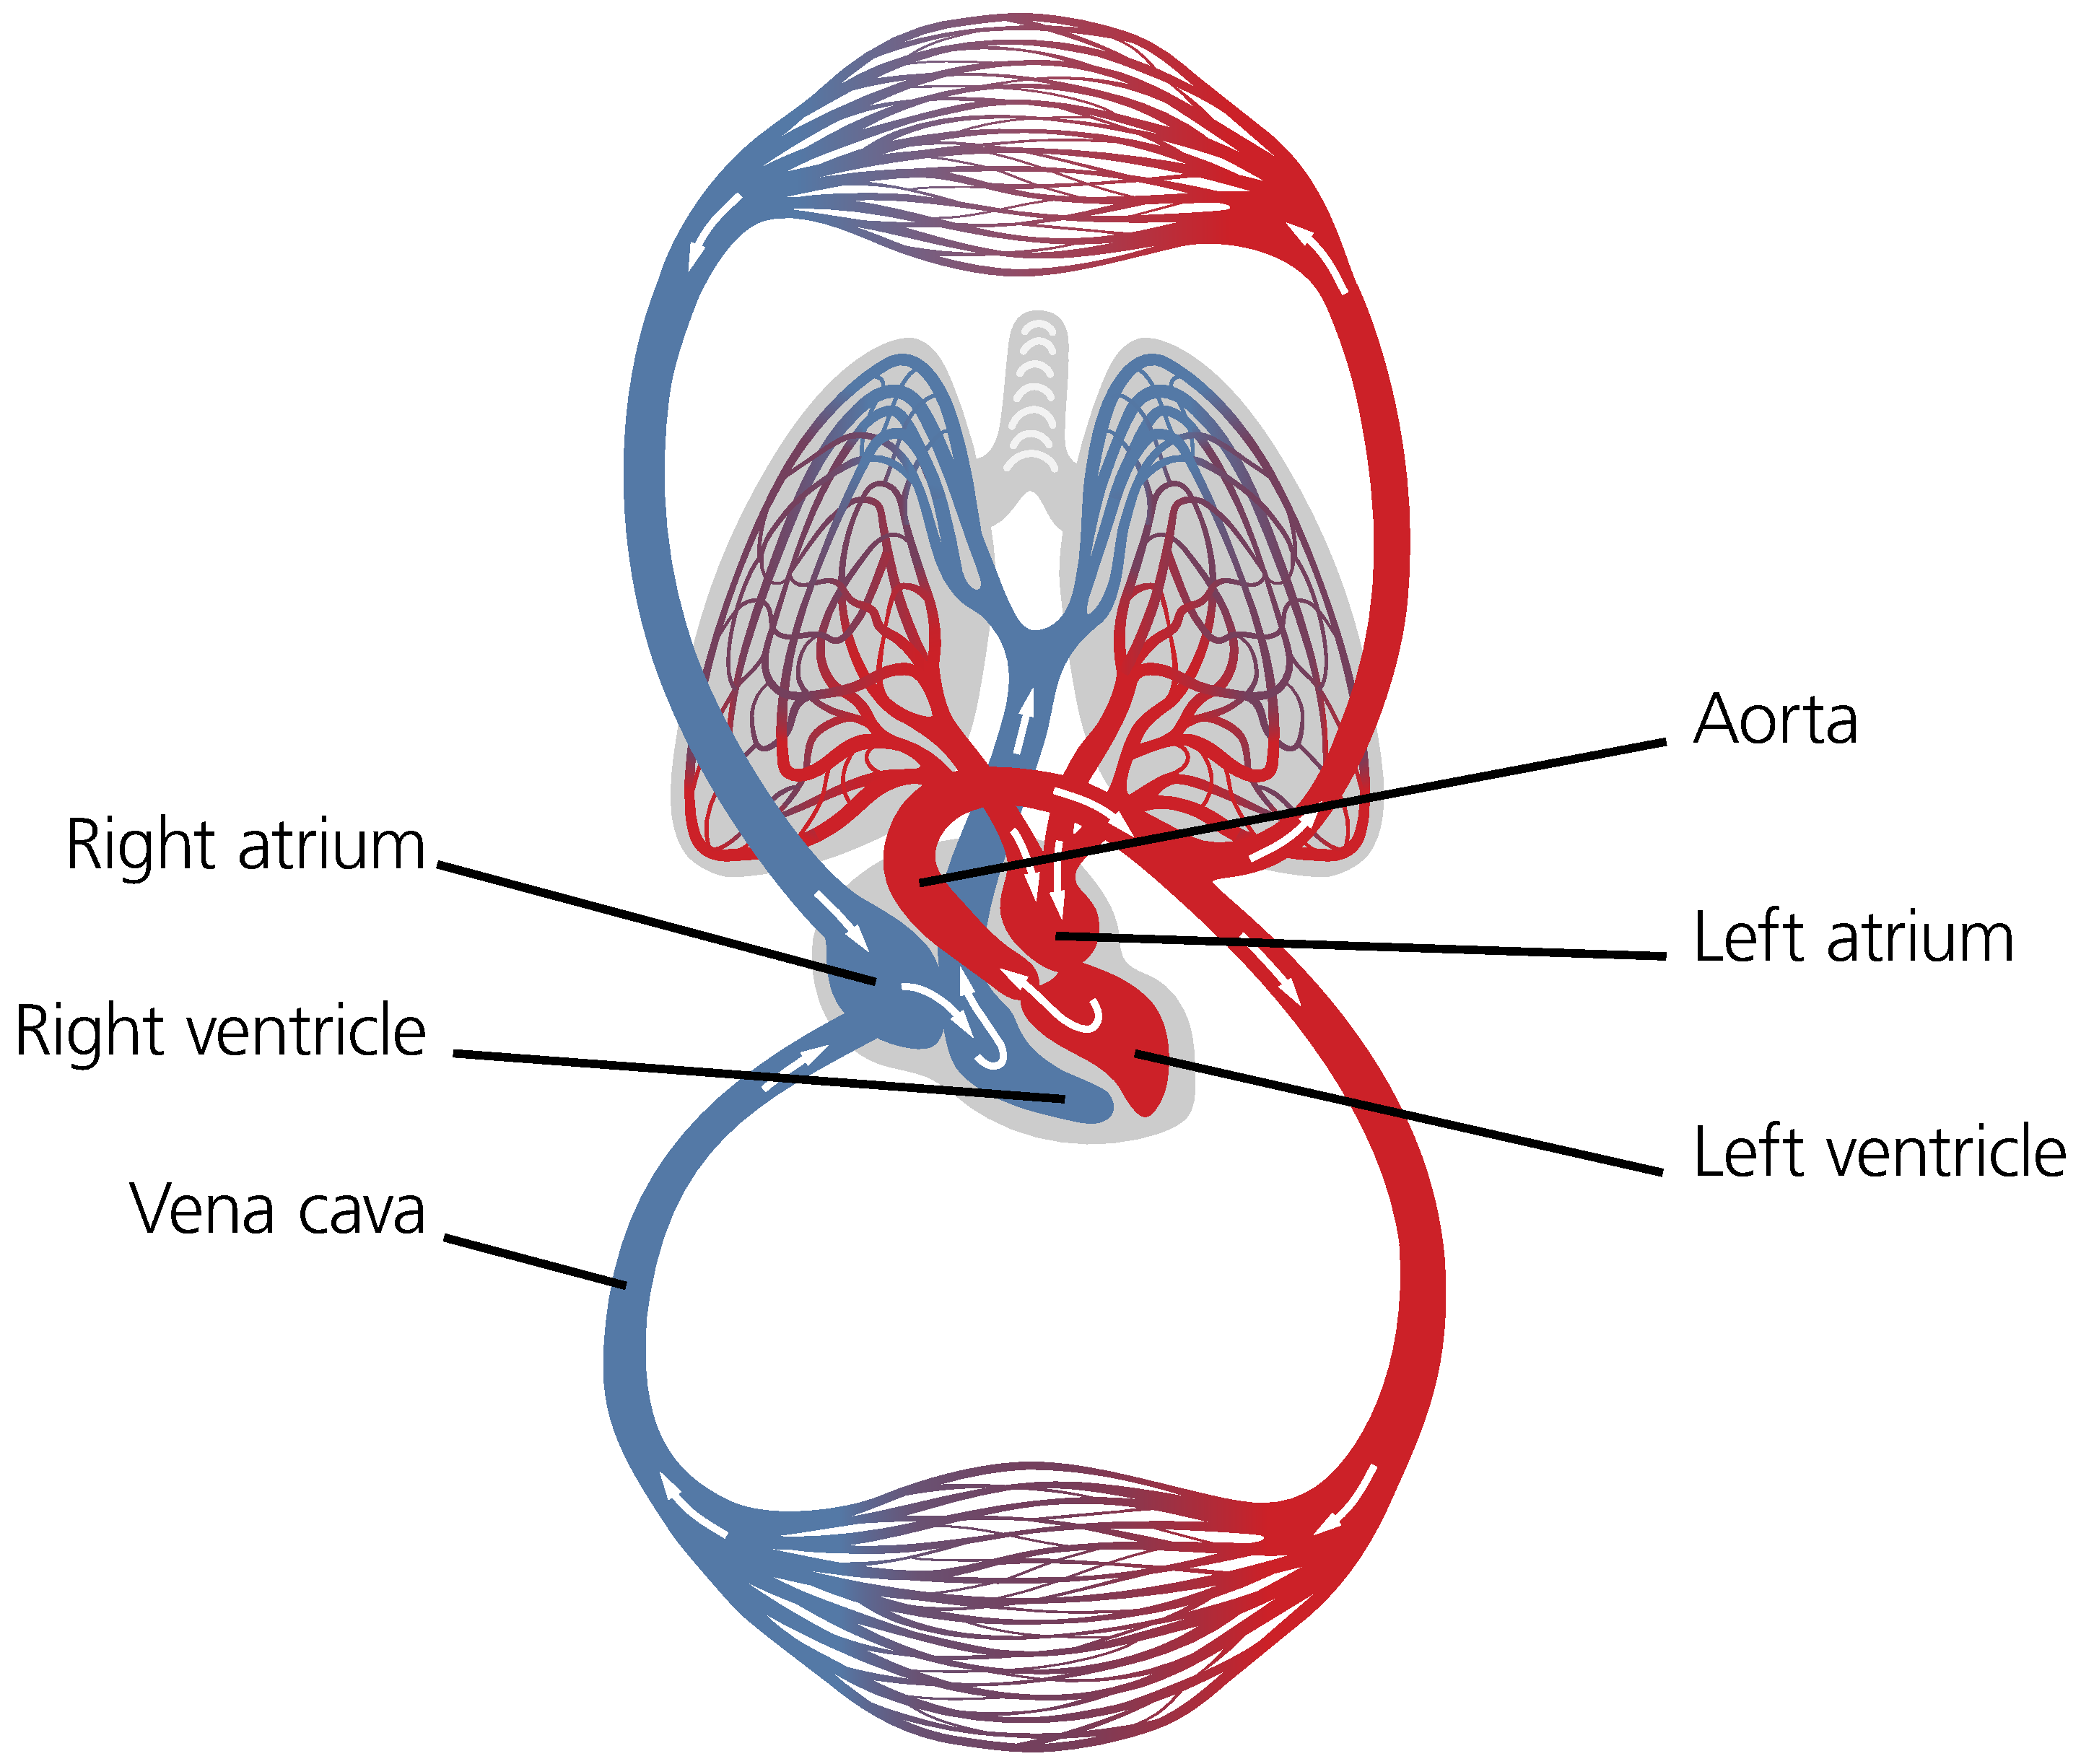
\includegraphics[width=0.75\textwidth]{circulation}
\caption{A schematic overview of the circulatory system. (Licensed under Adobe Stock Standard license)}
\label{fig:circulation}
\end{figure}

\sect{The heart}

\begin{figure}[htbp]
\centering
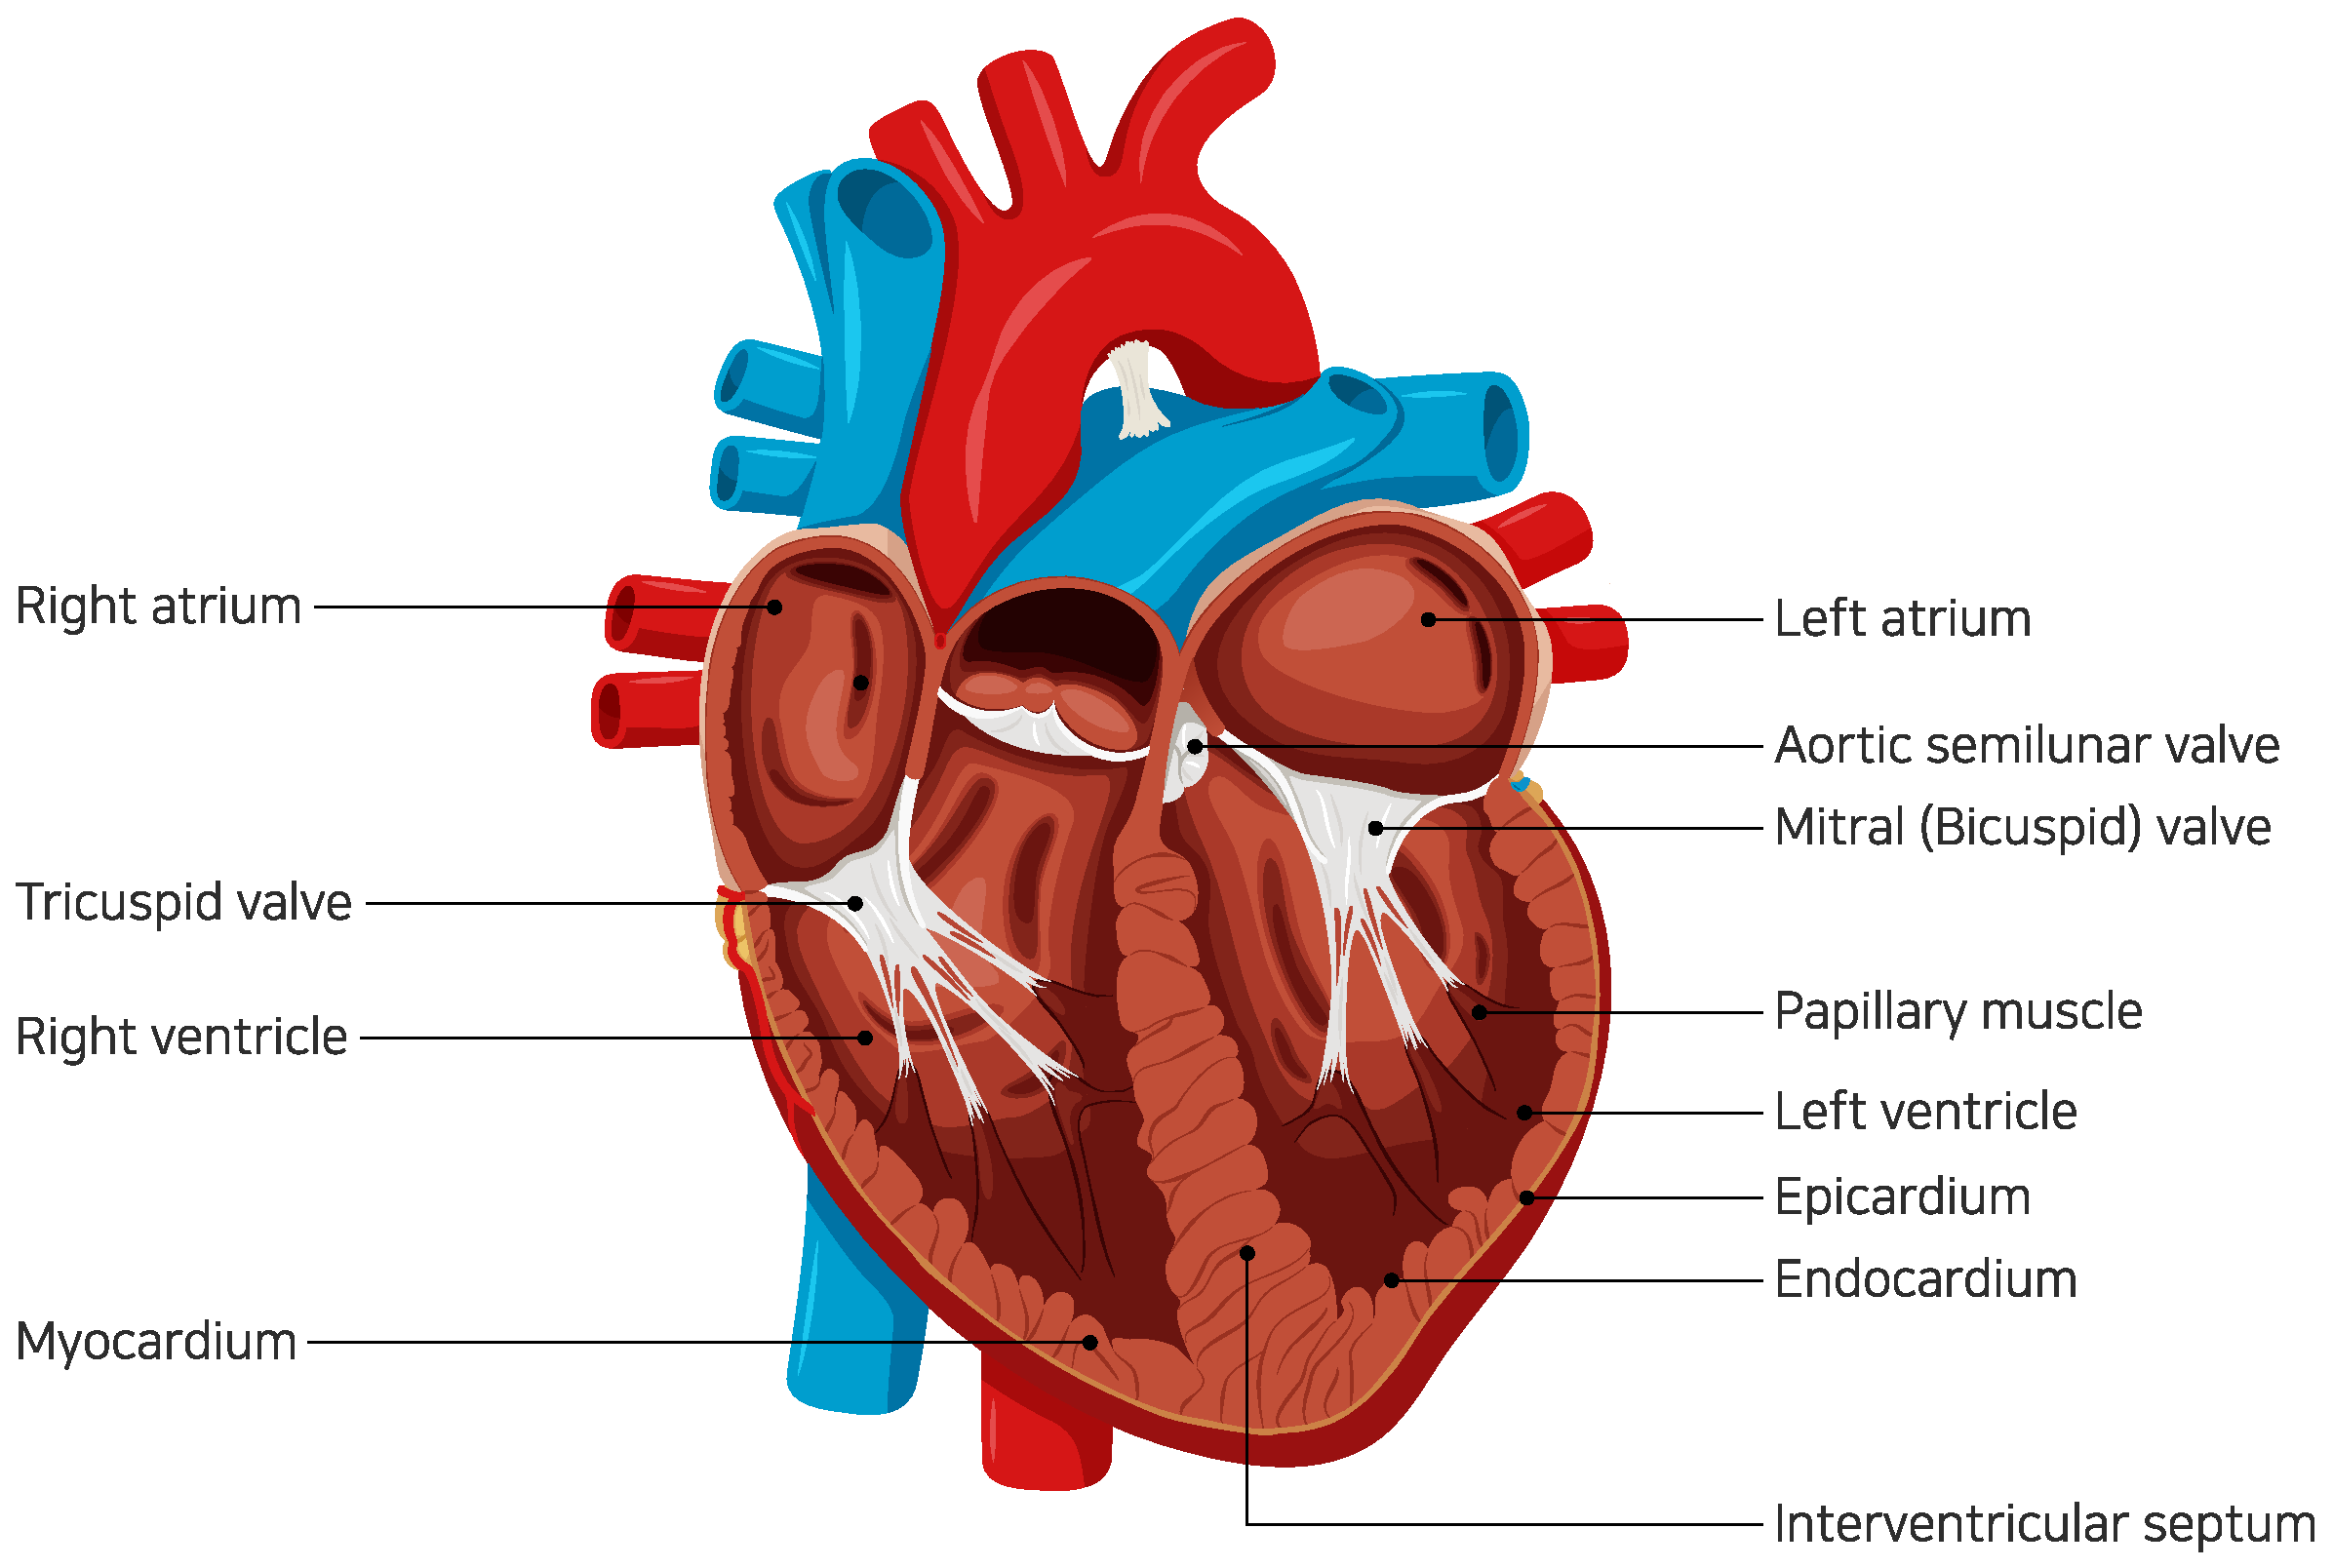
\includegraphics[width=0.75\textwidth]{heart}
\caption{A schematic overview of the human heart viewed from the front. (Licensed under Adobe Stock Standard license)}
\label{fig:heart}
\end{figure}
Both anatomically and functionally, the heart is divided into a left and a right side. Both sides have an atrium and a ventricle. The two ventricles are separated by the interventricular septum, see figure~\ref{fig:heart}.
\begin{figure}[tbp]
\centering
\includegraphics[width=0.75\textwidth]{valves}
\caption{A schematic overview of the valves of the heart viewed from above. (Licensed under Adobe Stock Standard license)}
\label{fig:valves}
\end{figure}
Venous blood is carried in the vena cava to the right side of the heart where it enters the right ventricle through the tricuspid valve, sometimes known as the right atrioventricular valve. From there, the blood is ejected through the pulmonary valve into the pulmonary circulation. Oxygenated blood then returns to the left atrium and enters the left ventricle through the mitral valve, sometimes known as the left atrioventricular valve. From the left ventricle, the blood then gets ejected back out into the systemic circulation through the aortic valve. 

\sect{Systolic function}
Systolic function refers to the heart's ability to pump forcefully enough to eject a sufficient amount of blood into the systemic circulation, to meet the oxygen and metabolic demand. The systolic function of the heart can be asserted by measuring a few key parameters, namely the end-diastolic volume (EDV)\Nomenclature{EDV}{End-diastolic Volume} and the end-systolic volume (ESV)\Nomenclature{ESV}{End-systolic Volume}. These measurements refer to the volume of blood in the left ventricle at the end of ventricular filling (end-diastole) and the end of ventricular contraction (end-systole), measured in ml. Using MRI, these measurements are acquired through manual and/or automatic segmentation of the left ventricle. From the ESV and the EDV, a few further parameters can be derived, namely the stroke volume (SV), \Nomenclature{SV}{Stroke volume} defined as $\textrm{SV} = \textrm{EDV} - \textrm{ESV}$, and the ejection fraction (EF), defined as \Nomenclature{EF}{Ejection fraction} $\textrm{EF} = \textrm{SV}/\textrm{EDV,}$ measured in percent.

\sect{Diastolic function}
Assessment of diastolic dysfunction using MRI remains challenging~\cite{Caudron2011}. Whereas some progress has been made in recent years~\cite{Flachskampf2015, Seemann2018}, the current non-invasive reference standard for assessing diastolic function is echocardiography~\cite{Nagueh2016}. The diagnosis encompasses both functional and structural parameters such as the peak in-flow velocity over the mitral valve during early filling (E) and late filling (A), and the peak velocity of the mitral annulus during early filling (e'). The E/A ratio is associated with the pressure gradient between the atrium and the ventricle, where an E/A ratio $>1$ is considered normal. The e' velocity reflects the velocity at which the myocardial muscle fibers lengthen in early diastole, and a reduced e' velocity may indicate diastolic dysfunction. The ratio $\textrm{E}/\textrm{e'}$ is also important as it is associated with the left ventricular filling pressure~\cite{Park2011}. See Figure~\ref{fig:echo} for an example of E, A and e' measurements using Doppler echocardiography. The remaining parameters used in echocardiographic assessment of diastolic dysfunction are the left atrial volume index (LAVI), \Nomenclature{LAVI}{Left atrial volume index} indexed to the body surface area (BSA),~\cite{Mosteller1987} \Nomenclature{BSA}{Body surface area} and the tricuspid regurgitant jet velocity. LAVI is an independent predictor of death and is associated with chronically elevated filling pressures~\cite{Pritchett2005}. The tricuspid regurgitant jet velocity, which through the simplified Bernoulli equation can be used to estimate the pressure gradient~\cite{Baumgartner2009}, which in turn can be related to pulmonary artery pressure as the sum of the pressure gradient and the right atrial pressure~\cite{Aduen2011}. Left atrial volume can easily be derived by CMR, and recent developments have suggested non-invasive measurements of pulmonary artery pressure derived by phase-contrast CMR~\cite{Reiter2013, Ramos2020}.
\begin{figure}[htbp]
\centering
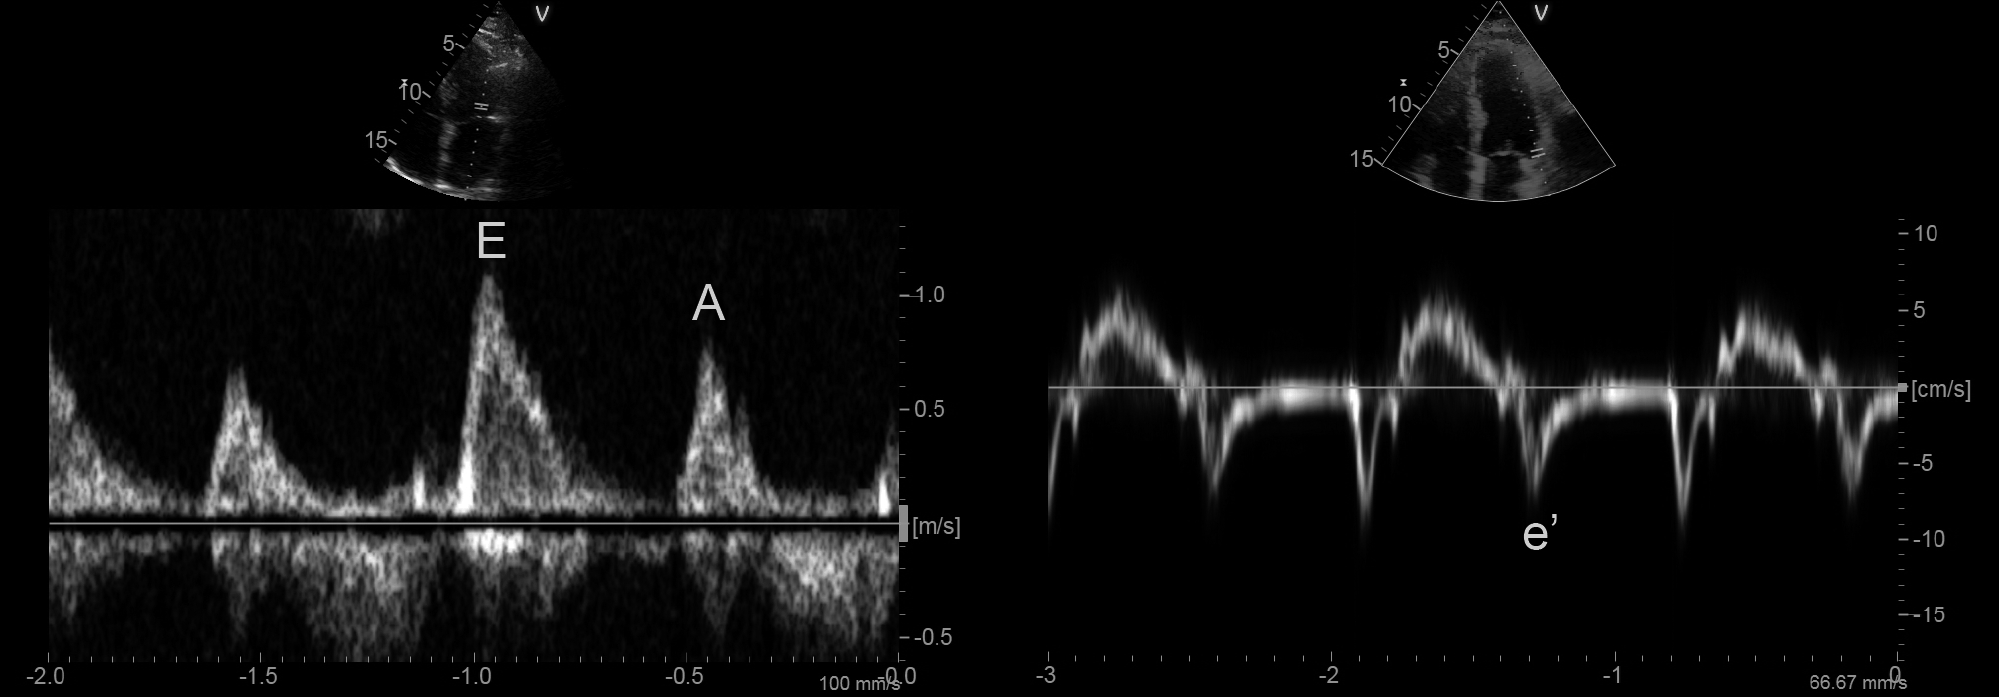
\includegraphics[width=\textwidth]{echo.png}
\caption{Example of key diastolic dysfunction parameters, such as trans-mitral inflow during early- and late filling (E \& A), and tissue velocity during early-filling (e') using Doppler echocardiography.}
\label{fig:echo}
\end{figure}
\sect{Heart failure}
Heart failure (HF)\Nomenclature{HF}{Heart failure} is defined as the condition when the heart cannot sufficiently pump blood to meet the oxygen demand under normal filling pressures~\cite{Hall2016}. Depending on the EF of the patient, heart failure can either be labeled heart failure with reduced ejection fraction, \Nomenclature{HFrEF}{Heart failure with reduced ejection fraction} or heart failure with preserved ejection fraction (HFpEF) \Nomenclature{HFpEF}{Heart failure with preserved ejection fraction}. Recent guidelines also specify a condition labeled heart failure with mid-range ejection fraction (HFmrEF) \Nomenclature{HFmrEF}{Heart failure with mid-range ejection fraction}\cite{Ponikowski2016}.

The cutoff values for the three types of heart failure are defined as
\begin{itemize}
    \item HFrEF: EF $<40\% $
    \item HFmrEF: $40\% \leq \textrm{EF} < 50\% $
    \item HFpEF: EF $\geq 50\% $
\end{itemize}
The pathophysiological mechanisms of HFpEF are somewhat contentious~\cite{Pfeffer2019}, yet most evidence points towards an impaired diastolic function~\cite{Nagueh2019}.

\sect{Pulmonary embolism}
Acute pulmonary embolism (PE) \Nomenclature{PE}{Pulmonary embolism} is a medical condition characterized by acute obstruction of the pulmonary arteries by a solid, liquid, or gaseous mass that originated somewhere else in the body. The most common cause is a thrombus formed in the deep veins, so-called deep vein thrombosis (DVT) \Nomenclature{DVT}{Deep vein thrombosis}~\cite{Goldhaber2012}. A thrombus can break loose and follow the veins back into the vena cava, where it may enter the right side of the heart and be ejected out into the arterial side of the pulmonary circulation, where it may cause a blockage of the blood flow as the vessels narrow. Whereas acute PE is a serious condition, the clinical presentation can be rather non-specific, with symptoms such as chest pain or shortness of breath~\cite{Hampson1995}. Therefore, imaging is an integral component in the diagnosis of pulmonary embolism~\cite{Bounameaux2010}. Typically, this is done with contrast-enhanced computed tomography angiography (CTA) \Nomenclature{CTA}{Computed tomography angiography}. There are many comorbidities for PE that may contraindicate CTA, thus making MRI an attractive alternative method for diagnosis of pulmonary embolism~\cite{Stein2011}. 
\begin{figure}[hbt]
\centering
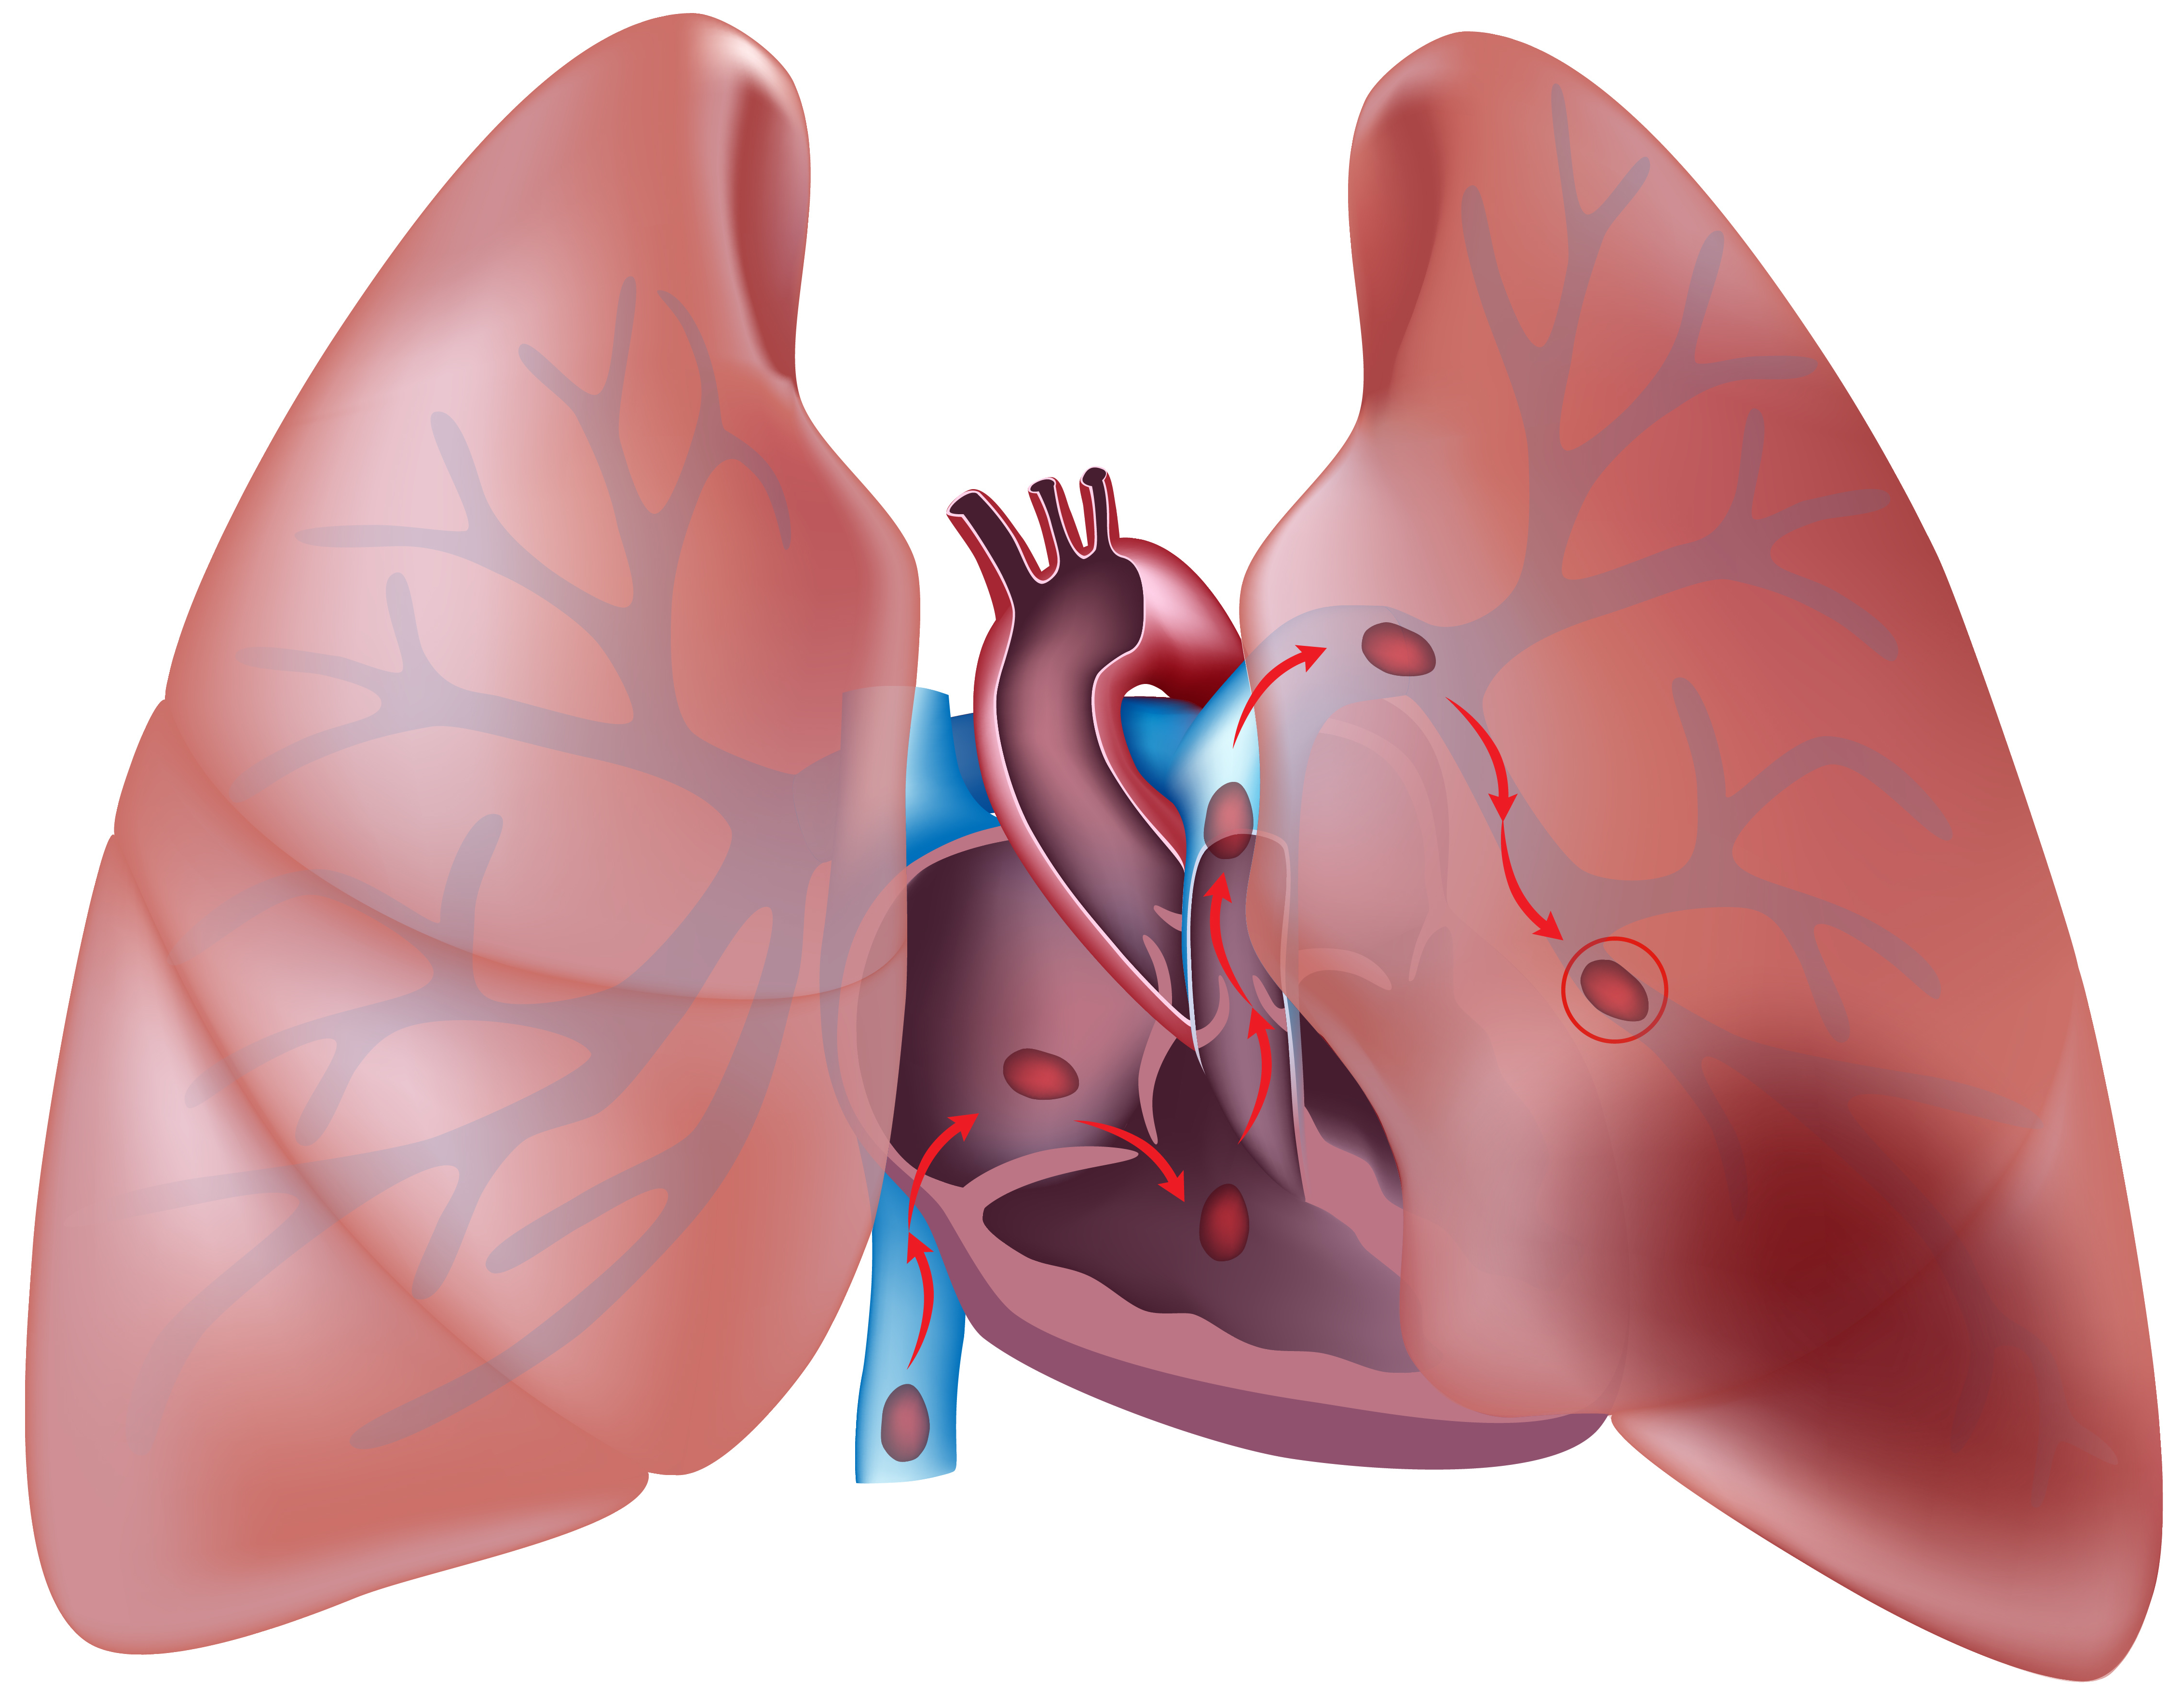
\includegraphics[width=\textwidth]{PE}
\caption{A schematic illustration of a thrombus originating in the deep veins entering the right side of the heart and ending up on the arterial side of the pulmonary circulation. (Licensed under Adobe Stock Standard license)}
\label{fig:pe}
\end{figure}

\chap{Magnetic Resonance}
This chapter is intended to give the reader a brief overview of the overwhelmingly large field that is nuclear magnetic resonance (NMR).\Nomenclature{NMR}{Nuclear Magnetic Resonance} The chapter introduces the quantum mechanical concept of spin but quickly moves on to describe magnetic resonance in terms of classical mechanics. Whereas it can be shown that many concepts touched upon in this thesis can equally well be described in terms of quantum phenomena, a measurement of the magnetic resonance signal does not make the spin ensemble collapse into a single particle eigenstate, hence motivating the adoption of a purely classical mechanical point of view~\cite{Hanson2008}.
\sect{Spin}
Spin is an intrinsic angular momentum present in all elementary particles. Elementary particles can be classified as either fermions or bosons. Fermions include quarks, leptons, and subatomic particles and nuclei composed of an odd number of quarks and leptons, such as protons and electrons. A common example of a boson would be the photon. All fermions have half-integer spin, i.e., the spin quantum number is an odd multiple of $1/2$ and are constrained by the Pauli exclusion principle that states that ``no two fermions can exist in identical quantum states''~\cite{Krane1988}. Spin gives rise to a magnetic dipole moment $\mu$ which is related to net spin angular momentum $\textbf{S}$ as
\begin{equation}
    \label{eq:spinmoment}
    \mu = \gamma\textbf{S}
\end{equation} where $\gamma$ is known as the gyromagnetic ratio. In the presence of an external static magnetic field, let us call it $B$, the magnetic dipoles will align themselves with the field in a precessing motion with the frequency
\begin{equation}
    \label{eq:larmor}
    \omega = \gamma B
\end{equation}
In magnetic resonance it often useful to consider a harmonic motion rather than an angular frequency, so the notation $\gbar = \frac{\gamma}{2\pi}$ is sometimes used. For a hydrogen nuclei, $\gammabar = 42.57$ MHz/T. The static field is often denoted $B_0$ and measured in Tesla, thus Eq.~\ref{eq:larmor} is often written as
\begin{equation}
    \omega_0 = \gamma B_0 \quad \textrm{or} \quad f_0 = \gbar B_0
\end{equation}
to denote the precession frequency when only a static magnetic field is present. Typical field strengths are $B_0 = 1.5$ T ($f_0 = 64$~MHz) and $B_0 = 3$ T ($f_0 = 128$~MHz).

In the quantum mechanical interpretation, alignment of the spins can be seen as a superposition of spin states. However, in the scope of this thesis, it is useful to consider the entire spin ensemble and its net magnetization, with corresponding net magnetization vector $\textbf{M} = (M_x, M_y, M_z)$~\cite{Levitt2001}. Due to thermal agitation and spin interactions the angular distribution of dipoles, the magnitude of $M$ at thermal equilibrium, denoted $M_0$ will be governed by a Boltzmann distribution, which predicts that
\begin{equation}
\label{eq:M0}
    M_0 = B_0\rho\frac{\gamma^2 \hbar^2}{4k_BT}
\end{equation}
where $\rho$ is the spin density, $\hbar$ is the reduced Planck constant, $k_B$ is Boltzmann's constant and T is the temperature in Kelvin.
\sect{Bloch equations}
The interaction between the net magnetization vector $\textbf{M}$ and a magnetic field $\textbf{B}$ can be described by the Bloch equation, which on a simplified form
can be expressed as
\begin{equation}
\label{eq:bloch1}
    \frac{d\textbf{M}}{dt} = \gamma(\textbf{M} \times \textbf{B})
\end{equation}
The simplification assumes that the orientation of $\textbf{M}$ is only due to the presence of an external magnetic field~\cite{Bloch1946}. At thermal equilibrium, the net magnetization only has a longitudinal component, i.e. $\textbf{M} = M_0(0, 0, 1)$. However, to be able to detect a signal, the net magnetization must be brought away from equilibrium, i.e. the spins need to be excited. This can be achieved by applying a time-varying magnetic field, let us call it $\textbf{B}_1(t)$, perpendicular to the static magnetic field $B_0$. The RF-field can be described as a \emph{linearly} polarized field
\begin{equation}
    \textbf{B}_1(t) = 2B_1^e(t)\textrm{cos}(\omega_{\textrm{rf}}\, t+\psi)\hat x
\end{equation}
where $B_1^e(t)$ is the pulse envelope function, e.g., a windowed sinc function, $\omega_{\textrm{rf}}$ is the carrier frequency and $\psi$ is the initial phase. In addition to the free precession about $B_0$, this will cause a forced precession of $\textbf{M}$ about $\textbf{B}_1(t)$. If the carrier frequency of $\textbf{B}_1(t)$ matches the Larmor precession frequency of the spins, know as the \emph{resonance condition}, it will cause the net magnetization vector to move in a spiral motion towards the transversal plane.

The linearly polarized field can be divided into two \emph{circularly} polarized fields
\begin{align}
  \textbf{B}_1(t) = B_1^e(t)\left(\textrm{cos}(\omega_{\textrm{rf}}\, t+\psi)\hat x - \textrm{sin}(\omega_{\textrm{rf}}\, t+\psi)\hat y \right) +
  \notag\\
     B_1^e(t)\left(\textrm{cos}(\omega_{\textrm{rf}}\, t+\psi)\hat x + \textrm{sin}(\omega_{\textrm{rf}}\, t+\psi)\hat y \right) \phantom{+}
\end{align}
where the first term is the resonant term which forces the precession, and the second term is an non-resonant term that only contributes to energy deposition. By using quadrature transmit coils, we can produce a circularly polarized field that only contains the resonant term
\begin{equation}
    \textbf{B}_1(t) = B_1^e(t)\left(\textrm{cos}(\omega_{\textrm{rf}}\, t+\psi)\hat x - \textrm{sin}(\omega_{\textrm{rf}}\, t+\psi)\hat y\right).
\end{equation}
As the frequency of the time-varying field typically resides in the radio frequency range, we refer to it as an RF-pulse. The angle between $\textbf{M}$ and the z-axis is characterized as the flip angle, and can be described as
\begin{equation}
    \label{eq:fa}
    \alpha = \gamma\int_0^\tau B_1^e(t)\,\dif t
\end{equation}
where $B_1^e(t)$ is the envelope function of effective field and $\tau$ is its duration~\cite{Bernstein2004}. Directly after the end of the RF-pulse, assuming the RF-pulse is applied along the positive $\hat x$ direction, the state of the system is as follows
\begin{equation}
	\textbf{B} =
	\begin{pmatrix}
		0\\0\\B_0\\
	\end{pmatrix}
\quad
\textrm{and}
\quad
	\textbf{M}(0) = M_0
	\begin{pmatrix}
		0\\\sin(\alpha)\\\cos(\alpha)\\
	\end{pmatrix},
\end{equation}
i.e. the only magnetic field present is the $B_0$ field along the z-axis and at time $t = 0$ the net magnetization has the magnitude which is equal to the magnitude of the equilibrium magnetization, denoted $M_0$, and forms an angle $\alpha$ to the transversal plane. The solution to Eq.~\eqref{eq:bloch1} is then
\begin{equation}
	\textbf{M}(t) = M_0
	\begin{pmatrix}
		\phantom{-}\cos(\omega_{0}\, t+\psi) \sin(\alpha) \\
		-\sin(\omega_{0}\, t+\psi) \sin(\alpha)\\
		\cos(\alpha) \\
	\end{pmatrix}
\end{equation}
which describes a precessing motion with the Larmor frequency. The transverse component, $\textbf{M}_{xy}$  can also be written in complex notation as
\begin{equation}
    M_{xy}(0) = M_0\sin(\alpha)\left( \cos(\omega_{0}\, t + \psi) - i\sin(\omega_{0}\, t + \psi) \right) = M_0\sin(\alpha)\, e^{-i\omega_{0}\, t}e^{-i \psi}
\end{equation}

To simplify the notation, a rotating frame of reference is often adopted, where the coordinate system rotates with the Larmor frequency. Figure~\ref{fig:blochplots_1} describes the process of excitation in both the static (laboratory) frame of reference and the rotating frame of reference.
\begin{figure}[htbp]
    \centering
    
\includegraphics[width=0.75\textwidth]{bloch_plot}
    \caption{The process of excitation can be visualized in both the laboratory frame of reference and the rotating frame of reference. The black arrow denotes the magnetization vector, and $\alpha$ denotes the flip angle.}
    \label{fig:blochplots_1}
\end{figure}
\sect{Relaxation}
In the previous section, we assumed that the orientation of $\textbf{M}$ was solely due to the presence of an external magnetic field $\textbf{B}_1$. However, there is also an interaction between the individual spins and the surrounding lattice, so-called \emph{spin-lattice} interactions, and interactions between spins with other spins, so-called \emph{spin-spin} interactions. These processes' will cause a loss of spin coherence in the transversal plane and regrowth of magnetization in the longitudinal plane in a process known as relaxation. The time constant that govern these two time courses are known as the \emph{spin-lattice relaxation time}, denoted $T_1$ and the \emph{spin-spin relaxation time}, denoted $T_2$. From Eq.~\ref{eq:larmor}, we can deduce that the precession frequency is dependent on the experienced magnetic field strength. This means that local variations in the magnetic field strength will cause spins to precess at slightly different frequencies, leading to a loss of coherence, and thus a loss of transverse net magnetization, which is different from the $T_2$-time. Therefore it is useful to define an ``apparent'' relaxation time, denoted $T_2^*$ defined as
\begin{equation}
    \label{eq:t2star}
    \frac{1}{T_2^*} = \frac{1}{T_2} + \frac{1}{T_2'}
\end{equation}
where $T_2'$ is the time constant that describes the loss of coherence that is attributed to local magnetic field variations. Depending on the type of pulse sequence used, the $T_2'$ effect may be negated, leaving the contrast to be affected only by $T_2$-relaxation. For the rest of this section, we will assume that the static magnetic field is homogeneous and that all loss of coherence can be attributed to $T_2$-relaxation.

As $T_1$ and $T_2$ relaxation are orthogonal processes (transversal and longitudinal) it is possible to decouple eq.~\ref{eq:bloch1} into two ordinary differential equations. Under the initial condition $\textrm{B} = (0,0,B_0)$ 
\begin{equation}
    \label{eq:decoupled_bloch_1}
    \frac{dM_z}{dt} = 0
\end{equation}
\begin{equation}
    \label{eq:decoupled_bloch_2}
    \frac{\dif\textbf{M}_{xy}}{\dif t} = \gamma ( \textbf{M}_{xy}\times \textbf{B})
\end{equation}
It's was previously stated in Eq.~\ref{eq:bloch1} that \textbf{M} was only affected by the presence of an external magnetic field, but from the previous discussion it's clear that this assumption does not hold, and subsequently Eq.~\ref{eq:bloch1} must be modified accordingly. As already described, the longitudinal growth rate is proportional to the difference between $M_0$ and $M_z$ by the proportionality constant $T_1$, meaning that Eq.~\ref{eq:decoupled_bloch_1} can be restated as
\begin{equation}
    \frac{\dif M_z}{\dif t} = \frac{1}{T_1}(M_0-M_z)
\end{equation}
which has the solution
\begin{equation}
    M_z(t) = M_z(0)e^{-t/T_1} + M_0(1-e^{-t/T_1})
\end{equation}
The transversal decay can be described by saying that $M_{xy}$ decreases by the time constant $T_2$, i.e. Eq.~\ref{eq:decoupled_bloch_2} is restated as
\begin{equation}
    \frac{\dif \textbf{M}_{xy}}{\dif t} = \gamma ( \textbf{M}_{xy}\times \textbf{B}) - \frac{1}{T_2}\textbf{M}_{xy}.
\end{equation}
Assuming that \textbf{B} is not time-dependent, i.e. that no RF-pulse is present, the solution can be written as
\begin{equation}
    M_{xy}(t) = M_{xy}(0)e^{-t/T_2}.
\end{equation}
Finally, we arrive at an expression for the magnetization after an RF-pulse with flip angle $\alpha$, considering relaxation, which can be described as
\begin{equation}
    M_z(t) = M_0\,\textrm{cos}(\alpha)e^{-t/T_1} + M_0(1-e^{-t/T_1})
\end{equation}
\begin{equation}
    M_{xy}(t) = M_0\,\textrm{sin}(\alpha)e^{-t/T_2}\,e^{-i\omega_{0}\,t}e^{-i\psi}
\end{equation}
\begin{figure}[hbtp]
    \begin{subfloat}
        \centering
        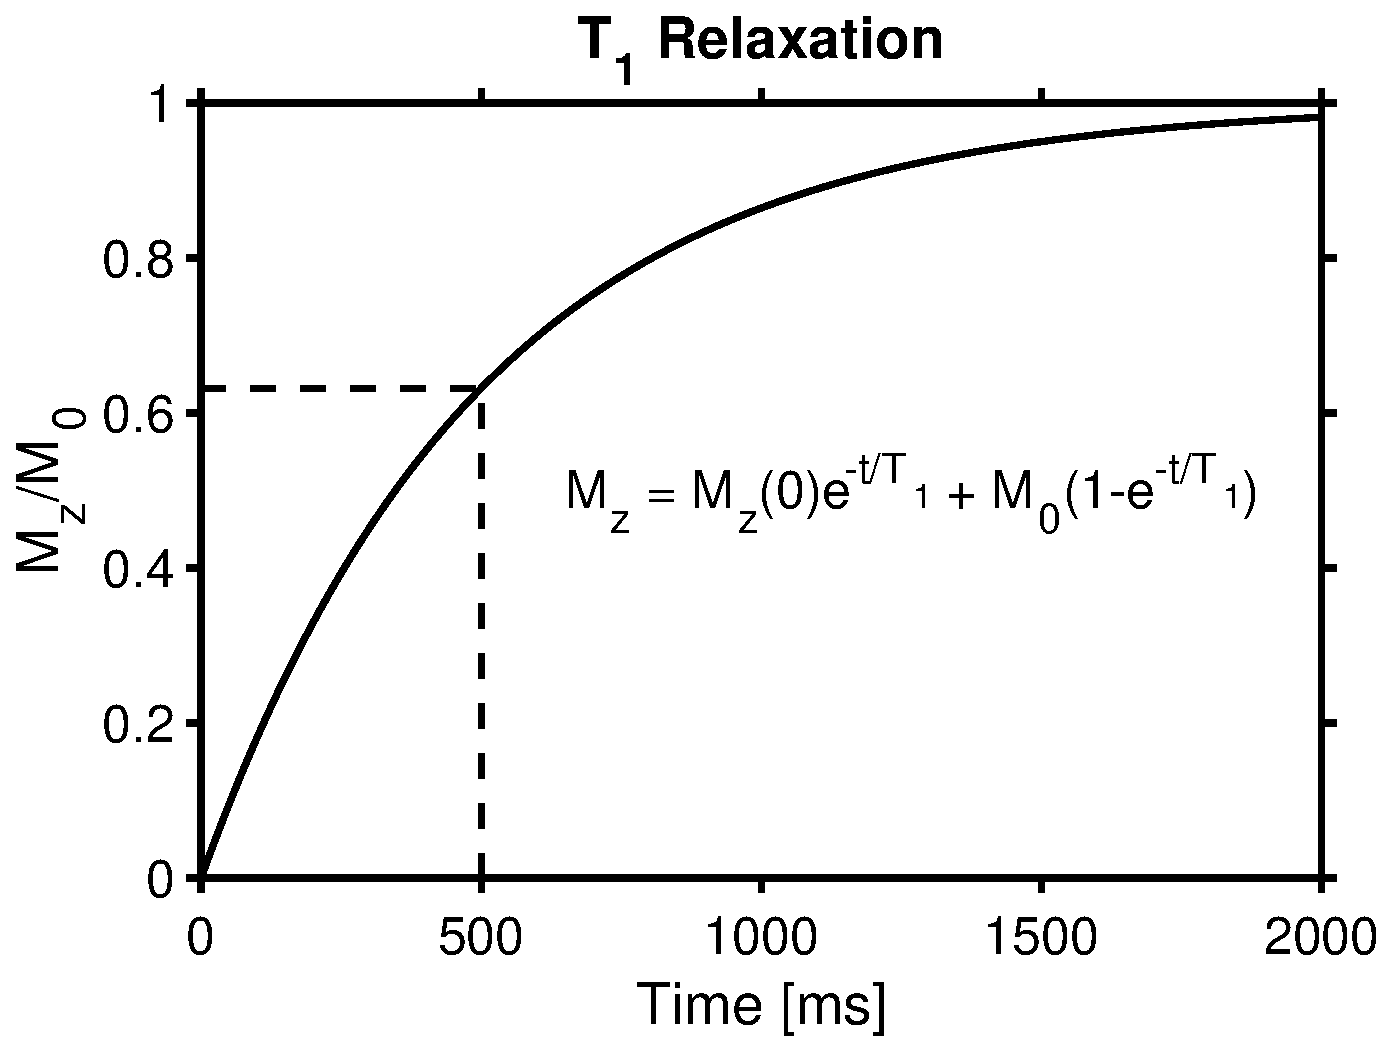
\includegraphics[width=0.49\textwidth]{t1}
    \end{subfloat}
    \begin{subfloat}
        \centering
        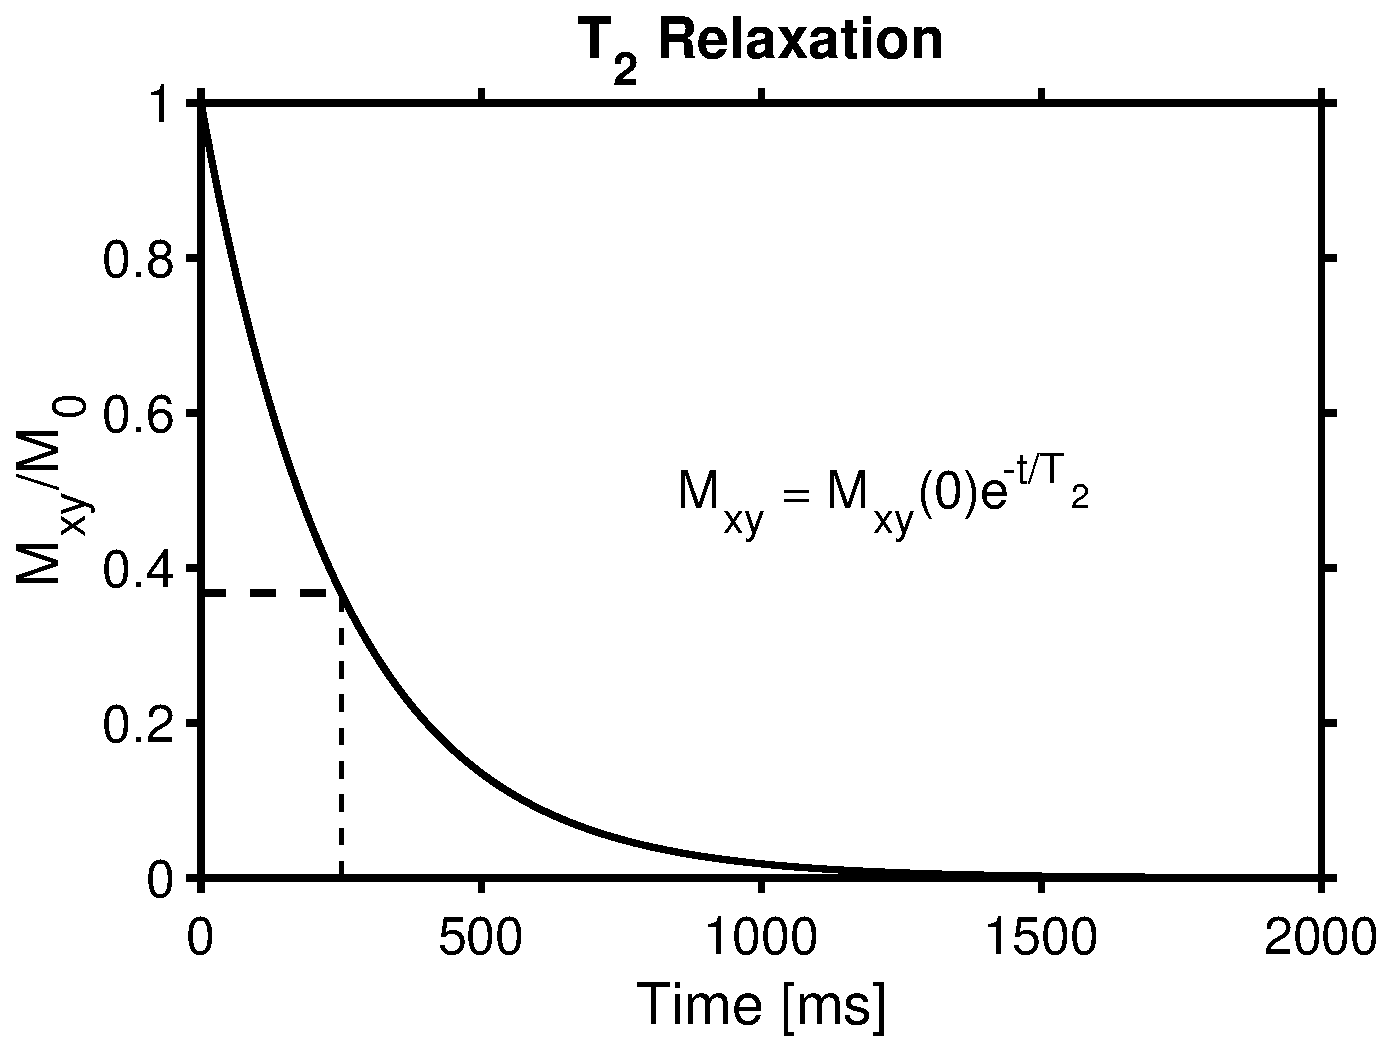
\includegraphics[width=0.49\textwidth]{t2}
    \end{subfloat}
    \caption{Bloch equation simulations of $T_1$ decay (left) and $T_2$ decay (right). The time constant $T_1$ is defined as the time at which $63\%$ of the longitudinal magnetization is recovered ($1-e^{-1} = 0.6321$) and $T_2$ is defined as the time when $37\%$ of the transversal magnetization remains ($e^{-1} = 0.3679)$. The simulation parameters were as follows: $T_1 = 500\textrm{ ms}, T_2 = 250\textrm{ ms}$, $M_z(0) = 0$, and $M_{xy}(0) = M_0$ }
    \label{fig:relaxation}
\end{figure}
\sect{Signal reception}
To receive a signal, we use sensitive receiver coils. The transverse magnetization will create a voltage in the receiver coils, in accordance with Faraday's law of induction
\begin{equation}
    V(t) = -\frac{\partial \Phi}{\partial t} = -\frac{\partial}{\partial t}\int_{\textrm{object}} \textbf{B}(\textbf{r})\cdot\textbf{M}(\textbf{r},t) \dif \textbf{r}
\end{equation}
where $\Phi$ is the magnetic flux, $\textbf{B}$ is the receiver coil sensitivity and $\textbf{r}$ is the location in space. By assuming a uniform sensitivity, calculating the partial derivative, and performing some simplifications we arrive at
\begin{equation}
    V(t) = -\int_{\textrm{object}} \omega(\textbf{r})M_{xy}(\textbf{r},0)e^{-t/T_2}\cdot\sin(-\omega(\textbf{r})t + \psi(\textbf{r}))\,\dif\textbf{r}
\end{equation}
The MR scanner uses what is know as phase sensitive detection. The voltage measured by the coil is demodulated by a sine and a cosine function which is on-resonance with the Larmor frequency, then low-pass filtered to obtain what is essentially the rotating frame of reference signal. In complex notation, the measured, demodulated, signal can be expressed as
\begin{equation}
    S(t) = \omega_0e^{i\pi/2}\int_{\textrm{object}}M_{xy}(\textbf{r},0)e^{-t/T_2(\textbf{r})}e^{-i\Delta \omega(\textbf{r})t}\dif \textbf{r}
    \label{eq:signal}
\end{equation}


%To excite and receive the signal, we use coils. One specific coil setup can be used for transmission (TX) \Nomenclature{TX}{Transmission} or for reception (RX), \Nomenclature{RX}{Reception} or both (TX/RX). The bird-cage "body coil" built into the bore of the MR scanner is a so called TX/RX-coil meaning that it can both be used both to excite the spins, and to receive signal. The body coil has a large reception volume, with a very uniform signal, albeit with a low signal-to-noise ratio (SNR). \Nomenclature{SNR}{Signal-to-noise ratio} Instead, phased array surface coils can be used to receive a signal with high SNR, but with an non-uniform reception field~\cite{Roemer1990}.

\sect{Free Induction Decay}
If a signal is acquired from the moment the excitation pulse was turned off, and until the signal had naturally decayed, one would obtain what is known as a free induction decay (FID) \Nomenclature{FID}{Free induction decay}~\cite{Hahn1953}. The FID would contain all signals in the imaging volume superimposed on each other. Using the FID, one could apply the inverse Fourier transform to obtain a frequency spectrum, representing the molecular content of the sample volume. Depending on the molecular makeup of the sample, several peaks might be visible, as the resonant frequency depends on the molecular environment of the protons, and in particular, the number of electrons shielding the nucleus. The Larmor frequency is sometimes expressed as
\begin{equation}
    \omega_0 = \gamma B_0(1-\sigma)
    \label{eq:larmor_shield}
\end{equation}
where $\sigma$ is the shielding constant. The difference is resonant frequency is called chemical shift, denoted $\delta$, and is measured in parts per million (ppm). The difference between water and fat, for instance, is about 3.5 ppm~\cite{Harris2001}.

\sect{Gradients and spatial encoding}
To create an image from the acquired signal, the MR signal must be spatially encoded. This is achieved by superimposing spatially variant gradient field over the static magnetic field $B_0$, such that $B = B_0 + \textbf{G}$, where the gradient field $\textbf{G} = (G_x,G_y,G_z)$ can be described as 
\begin{equation}
    G_x = \frac{\dif B}{\dif x}, \quad G_y = \frac{\dif B}{\dif y}, \quad G_z = \frac{\dif B}{\dif z}. 
\end{equation}

The last exponential term in Eq.~\ref{eq:signal} represents the spatial variation precession frequency. This can be defined as
\begin{equation}
    \Delta \omega(\textbf{r})\,t = \gamma\textbf{G}\cdot\textbf{r} = 2\pi\textbf{k}\cdot\textbf{r}.
\end{equation}
Instead of angular frequencies $\omega$, we introduce $\textbf{k}$ as a representation spatial frequencies, where
\begin{equation}
    \textbf{k}(t) = \gbar\int_0^t \textbf{G}(\tau)\,\dif\tau
\end{equation}

This formalism is the foundation of what is known as the k-space~\cite{Twieg1983, Ljunggren1983}. The k-space can be seen as the Fourier transform of the image. The k-space has an inverse relationship with the image, e.g., the sampling distance in k-space ($\Delta k$) is proportional to the field of view \Nomenclature{FOV}{Field of view}(FOV) 
\begin{equation}
    \Delta k = \frac{1}{\textrm{FOV}}
\end{equation}
and the extent of the k-space is related to the resolution in image space,
\begin{equation}
    \Delta w = \frac{1}{2\, k_{\textrm{max}}}
\end{equation}
where $\Delta w$ is the voxel size in k-space, assuming a k-space extent of $\pm k_{\textrm{max}}$, see Figure~\ref{fig:kspace}.
\begin{figure}[htbp]
    \centering
    \includegraphics[width=\textwidth]{kspace2}
    \caption{The magnitude of the k-space, in logarithmic scale (left) and the magnitude of the corresponding image (right). The inverse Fourier transform is used to transform between the k-space and the image space. \emph{Note:} The size of $\Delta k$ and $\Delta w$ are exaggerated for clarity.}
    \label{fig:kspace}
\end{figure}

Three types of spatial encoding are commonly used
\begin{itemize}
    \item Slice selection
    \item Phase encoding
    \item Frequency encoding
\end{itemize}

For the sake of this discussion, we assume that slice selection is made along the $z$-direction, phase encoding along the $y$-direction, and frequency encoding along the $x$-direction.
\subsect{Slice selection}
Only spins with a precession frequency $\omega$ that matches the carrier frequency $\omega_{\textrm{rf}}$  of $\textbf{B}_1$ will be excited. By applying a gradient along the z-axis, the selected slice will be at the position
\begin{equation}
    z = \frac{\omega - \gamma B_0}{\gamma G_z}
\end{equation}
in relation to the isocenter.
\subsect{Phase encoding}
The phase encoding gradient is switched on for a time $\tau$ along the phase encoding direction. During this time, spins will precess with different frequencies, resulting in a linear phase difference at the time when the phase encoding gradient is turned off. This phase difference can be described as
\begin{equation}
    \phi(x,y) = \gamma G_y \tau y
\end{equation}
\subsect{Frequency encoding}
During the signal acquisition, a gradient will be switched on creating a linear difference in precession frequency, which can be described as
\begin{equation}
    \omega(x,y) = \gamma G_x x
\end{equation}

%\sect{Magnetic Resonance Imaging}
%The concept of NMR was initially used as non-invasively measure the magnetic properties of samples, such as the magnetic moment~\cite{Rabi1938} or the relaxation time~\cite{Hahn1949}. However, in 1973 Lauterbur paved the way for magnetic resonance imaging with his seminal paper on using local magnetic field gradients to form an image~\cite{Lauterbur1973}.
\sect{Pulse sequences}
The order and timing in which the RF-pulses and gradients are played out is referred to as a pulse sequence. The pulse sequences can roughly be divided into two families; spin echo and gradient echo. The difference is how the \emph{echo} is formed. In a spin echo sequence, the echo is formed by applying a refocusing $180^\circ$ RF-pulse at $\textrm{TE}/2$, whereas gradient echo relies on the gradients alone to form the echo. A major difference between the two is that in a gradient echo pulse sequence, the transversal magnetization will experience $T_2^*$ decay, where the refocusing pulse of a spin echo pulse sequence would cancel out the $T_2'$ effects, leaving the transversal magnetization affected by $T_2$ alone.

For the rest of this thesis, only gradient echo pulse sequences will be considered. A common example of a gradient echo pulse sequence is Fast Low Angle Shot (FLASH) \Nomenclature{FLASH}{Fast low angle shot}. The sequence is executed with a low flip angle, and a short TR which is finished by a spoiler to dephase any residual magnetization before the next excitation. The signal equation for a FLASH sequence is given by
\begin{equation}
    S \propto \frac{\sin(\alpha)(1-e^{-\textrm{TR}/T_1})}{1-\cos(\alpha)\,e^{-\textrm{TR}/T_1}}e^{-\textrm{TE}/T_2^*}
    \label{eq:flash}
\end{equation}
By taking the partial derivative of S with respect to $\alpha$, the optimal flip angle for a FLASH sequence, sometimes known as the Ernst angle \cite{Ernst1966}, is found to be
\begin{equation}
    \alpha = \textrm{acos}\left ( e^{-\textrm{TR}/T_1} \right ).
\end{equation}
A schematic example of a gradient echo pulse sequence can be seen in Figure~\ref{fig:gre}.
\begin{figure}[htbp]
    \centering
    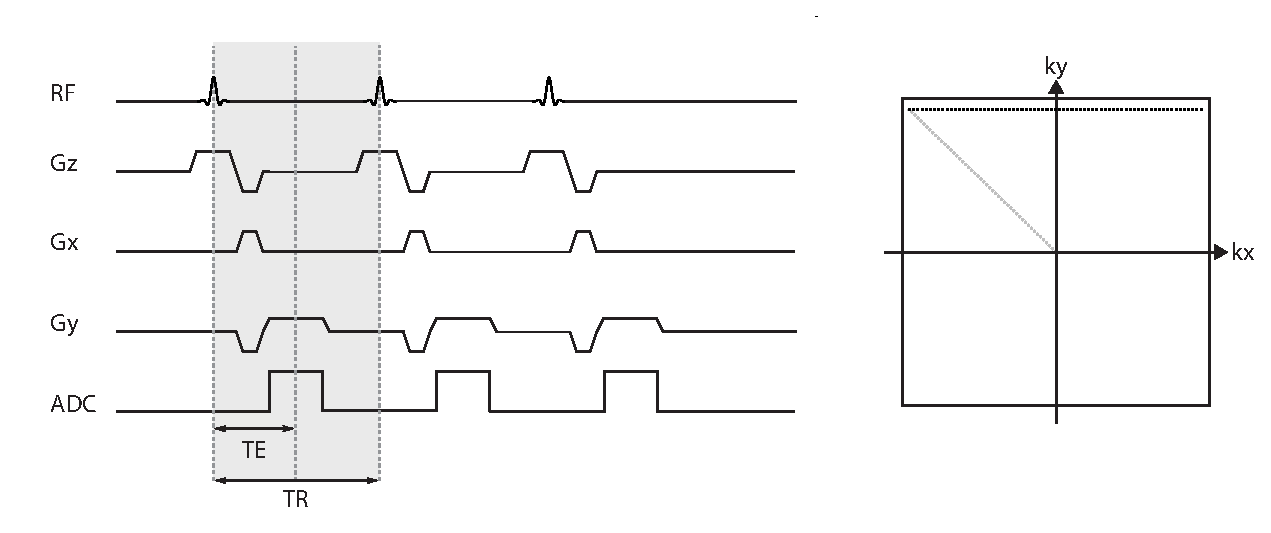
\includegraphics[width=\textwidth]{gre2}
    \caption{A schematic diagram of a gradient echo pulse sequence (left). The shaded box indicates one repetition. The RF pulse envelope in this example is a Hamming windowed sinc function, designed using John Pauly's RF design toolbox~\cite{Pauly1991}. In this figure, the gradient spoilers are omitted for brevity. A representation the k-space trajectory (right). The gray dotted line denotes the effect of the phase encoding gradient and the readout prewinder. The black dotted line denotes the readout of one k-space line.}
    \label{fig:gre}
\end{figure}
\sect{bSSFP}
The concept of Steady State Free Precession (SSFP, also known as FISP or FFE) \Nomenclature{SSFP}{Steady State Free Precession} \Nomenclature{FISP}{Fast imaging with steady state precession} \Nomenclature{FFE}{Fast field echo} predates magnetic resonance imaging. The concept was introduced as method to improve signal-to-noise ratio (SNR)\Nomenclature{SNR}{Signal-to-noise ratio} of NMR-measurements~\cite{Carr1958}. In the seminal paper, it's noted to have properties similar to that of a spin echo~\cite{Hahn1950}. In imaging, the SSFP method is often used with balanced gradients over one TR, i.e. the TE $= 2\,$ TR, and the gradient moment is nulled over one TR. In these cases, the sequence is referred to as balanced SSFP (bSSFP), TrueFISP, FIESTA \Nomenclature{FIESTA}{Fast imaging employing steady state acquisition} or balanced-FFE. \Nomenclature{bSSFP}{Balanced Steady State Free Precession} The bSSFP signal comprises both gradient echos, spin echoes and stimulated echos~\cite{Scheffler2003a,Scheffler2003b}. Compared to the FLASH method, bSSFP uses much higher flip angles, which may lead to more patient heating~\cite{Srinivasan2015}.

The signal equation for bSSFP can be expressed as
\begin{equation}
    S \propto \frac{\sin(\alpha)(1-e^{-\textrm{TR}/T_1})e^{-\textrm{TE}/T_2}}{1-(e^{-\textrm{TR}/T_1}-e^{-\textrm{TR}/T_2})\cos(\alpha)-(e^{-\textrm{TR}/T1})(e^{-\textrm{TR}/T_2})}
    \label{eq:bssfp1}
\end{equation}
In bSSFP, $\textrm{TE} = 2\,\textrm{TR}$, so it's usually safe to assume that $\textrm{TR} \ll T_1$. This means that we can disregard any TR-dependence, and subsequently simplify the equation to
\begin{equation}
    S \propto \frac{\sin(\alpha)e^{-\textrm{TE}/T_2}}{1+\cos(\alpha)+(1-\cos(\alpha))(T_1/T_2)}
    \label{eq:bssfp2}
\end{equation}
From Eq.~\ref{eq:bssfp2} it is apparent that the contrast is dependent on the ratio $T_2/T_1$~\cite{Huang2002}. This contrast weighting have been proven useful in cardiovascular imaging, where it provides a strong contrast between myocardium and blood~\cite{Caudron2011, Bieri2013}. 
\begin{figure}
    \centering
    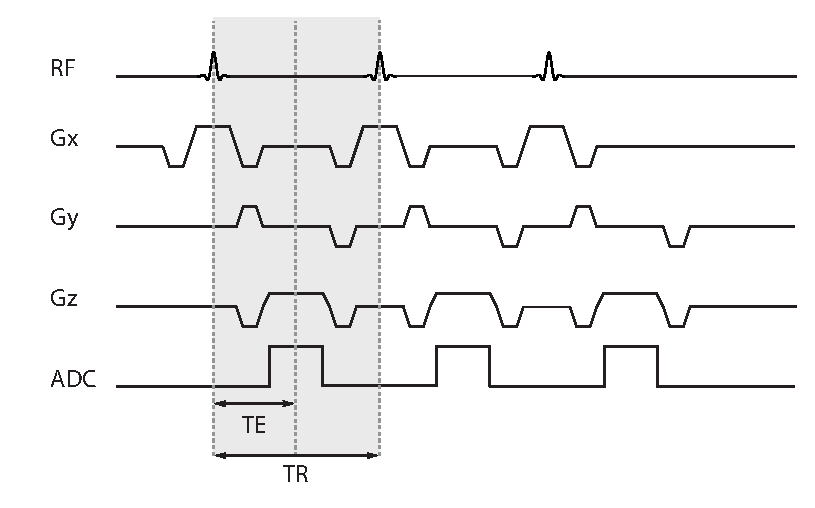
\includegraphics[width=0.75\textwidth]{bssfp_sequence}
    \caption{The gradient echo pulse sequence diagram from Figure~\ref{fig:gre} is here modified to describe a balanced steady state free precession pulse sequence. Note the addition of the balancing gradients that nulls the gradient moment on each axis over the repetition time, indicated by the shaded box. Note: This is a schematic representation of the pulse sequence diagram, and some gradients may not be to scale.}
    \label{fig:bssfp}
\end{figure}
Similar to the gradient echo method previously discussed, bSSFP is a steady-state method. To establish steady state as rapidly as possible, a preparatory ``$\alpha/2-\textrm{TR}/2$''-module is often used where only half of the flip-angle and half the repetition time is used in the first repetition~\cite{Deiming1994:ISMRM}. Figure~\ref{fig:blochplots_2} shows the transient steady-state when an ``$\alpha/2-\textrm{TR}/2$''-module is properly executed, and what happens when the magnetization is not properly prepared. An alternative approach is to use a ramp of linearly increasing RF-pulses~\cite{Nishimura2000:ISMRM, Deshpande2003} or a Kaiser-windowed ramp~\cite{LeRoux2003}.
\sect{Eddy currents in bSSFP}
Any imaging sequence will be affected by eddy currents, however in bSSFP, these effects take on a particular appearance. In the bSSFP method the RF-pulse phase is incremented by $180^\circ$ prior to each excitation. Assuming that the phase accrual is constant from TR to TR, a transversal steady state can be established over a $2 \textrm{TR}$ phase cycle, in addition to the longitudinal steady-state that is common to other gradient echo based methods. If this phase cycle is perturbed it may induce long-lived oscillations in the steady state signal. Figure~\ref{fig:blochplots_3} demonstrates what happens when a small phase perturbation is introduced into the bSSFP signal. Such phase perturbations can also come from other sources, such as flow \cite{Lagerstrand2009}, with similar effects on the steady state signal.
\begin{figure}
    \centering
    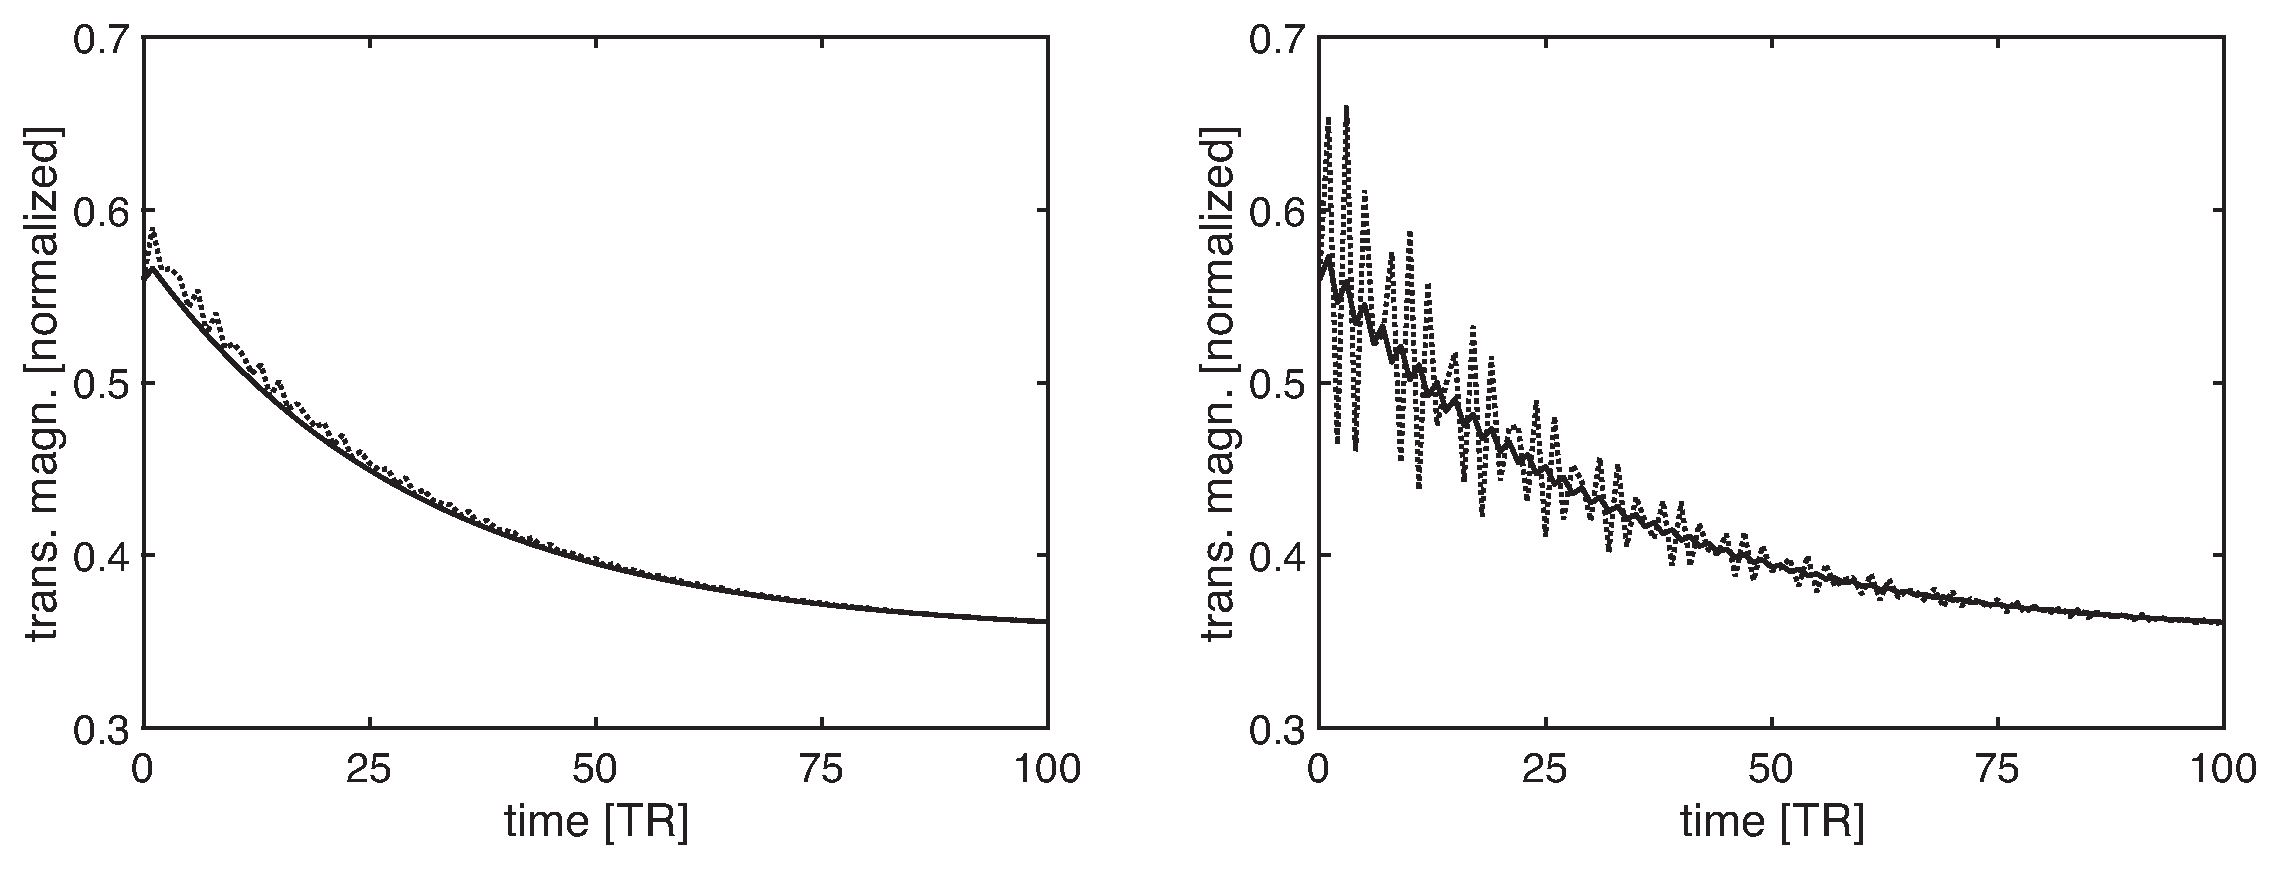
\includegraphics[width=\textwidth]{bieri1}
    \caption{Bloch-simulated time evolution during transient steady-state. The readout is initiated using an $\alpha/2-\textrm{TR}/2$ magnetization preparation (left) and without a shortened repetition time (right). The dashed line denotes the signal evolution off resonance ($30^\circ/\ \textrm{TR}$) and the solid line the signal evolution on resonance ($0^\circ/\ \textrm{TR}$). The simulation parameters were as follows: $\textrm{TE}/ \textrm{TR} = 1.75/3.5$ ms, $ \textrm{T}_1 = 140$ ms, $\textrm{T}_2 = 70$ ms, $\alpha = 70^\circ$. The right image is adapted from~\cite{Bieri2005a}.}
    \label{fig:blochplots_2}
\end{figure}
\begin{figure}
    \centering
    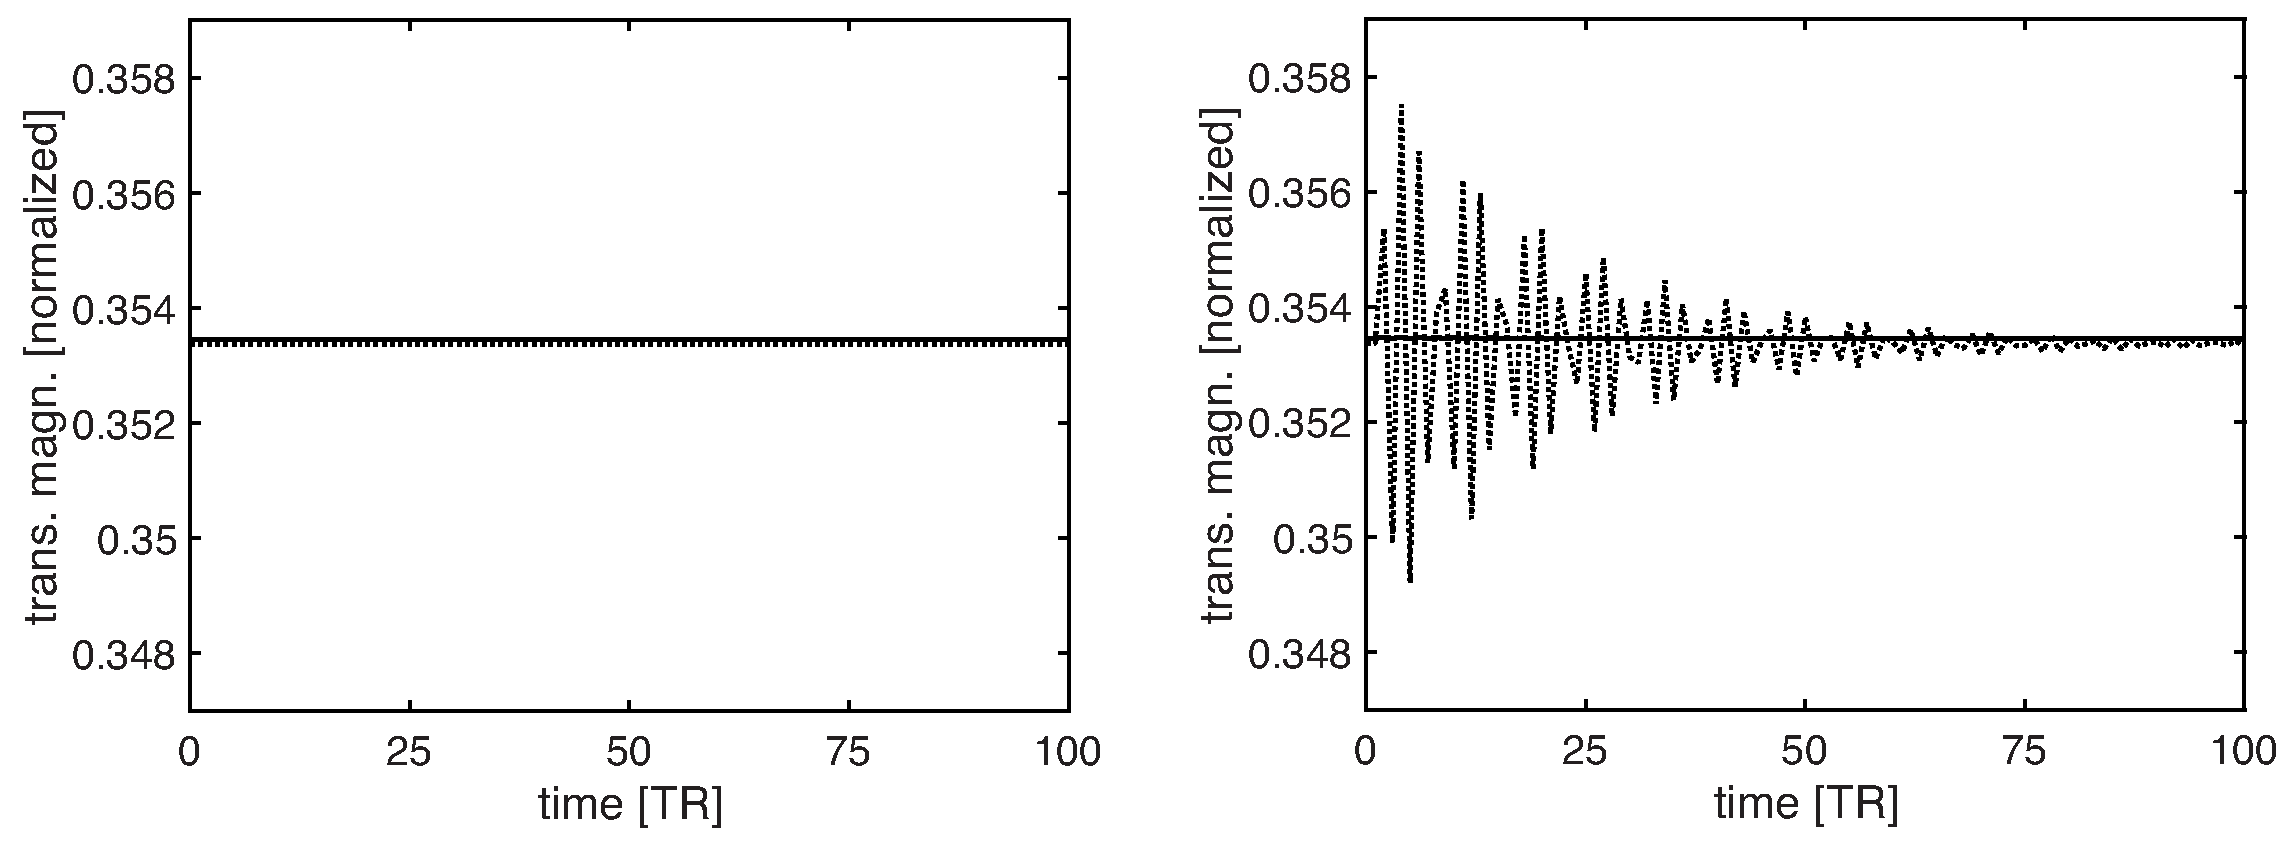
\includegraphics[width=\textwidth]{bieri2}
    \caption{Bloch-simulated time evolution at a stable steady-state (left), and with an initial phase perturbation of $1^\circ$ at time = 0 TR (right). The dashed line denotes the signal evolution off resonance ($30^\circ/\ \textrm{TR}$) and the solid line the signal evolution on resonance ($0^\circ/\ \textrm{TR}$). The simulation parameters were the same as in Figure~\ref{fig:blochplots_2}. Images are adapted from~\cite{Bieri2005a}.}
    \label{fig:blochplots_3}
\end{figure}

\sect{Radial imaging}
Conventionally, k-space is sampled on a Cartesian grid. However, the very first MR imaging method was based on projection imaging, similar to computed tomography \cite{Lauterbur1973}. By rotating the readout gradient in the physical coordinate system, a projection of the object was obtained. In the trajectory formalism, this can be likened to reading radial lines through the center of k-space. These radial lines are often referred to as spokes. The reconstruction of radial images generally requires an extra step compared to Cartesian image reconstructions. The non-Cartesian k-space cannot readily be transformed to image space using the fast Fourier transform algorithm (FFT), \Nomenclature{FFT}{Fast Fourier transform} which requires uniformly spaced sampling points. A common solution is to ``regrid'' the data onto a uniform grid, either through linear interpolation, or using a convolution kernel~\cite{Jackson1991}, see Figure~\ref{fig:gridding}. Two alternative methods are to calculate a non-uniform Fourier transform~\cite{Sarty2001}, or to use GRAPPA weights for the interpolation of the sampling points~\cite{Seiberlich2007}.
\begin{figure}[htbp]
    \centering
    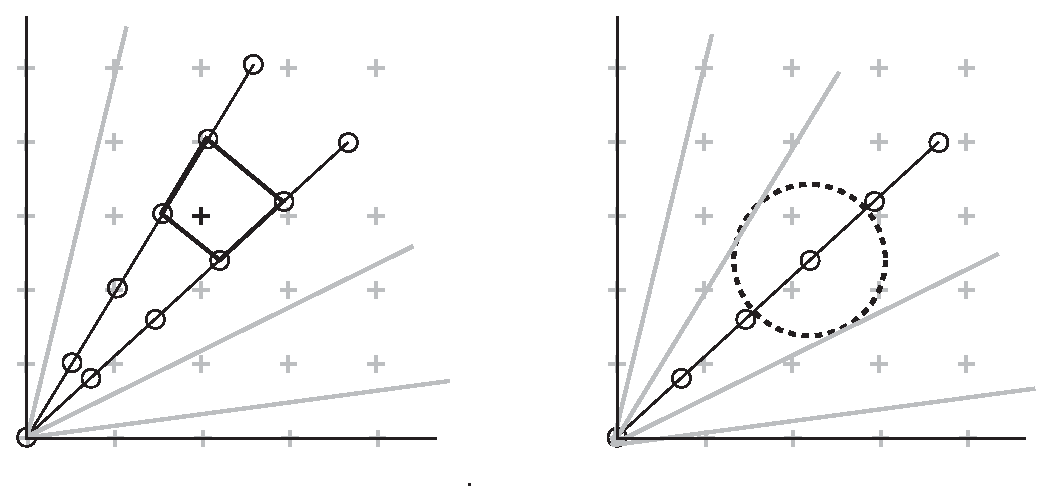
\includegraphics[width=\textwidth]{gridding}
\caption{A schematic overview of grid-driven (left) and data-driven (right) interpolation of sampling points onto a rectilinear grid. In the grid-driven approach, the value at each grid point (crosses) is found using bi-linear interpolation of the adjacent radial sample points (solid circles). In the data-driven approach, each radial sampling point is distributed onto the grid using kernel interpolation (dashed circle).}
    \label{fig:gridding}
\end{figure}
Using radial sampling, the density of the sampling points will be highest in the middle and decrease as a function of distance. A common approach is to use a linear ramp, or a Ramachandran-Lakshminarayanan (Ram-Lak) filter~\cite{Ramachandran1971}, to make the k-space density more uniform. However, for high undersampling factors, or for highly non-uniform k-space distributions, linear methods may not be sufficient. As an alternative, iterative methods based on gridding the trajectory have been proposed~\cite{Pipe1999}, see Figure~\ref{fig:pipe}. Analytical approximations have also been proposed~\cite{Nielles-Vallespin2007}. 
\begin{figure}
    \centering
    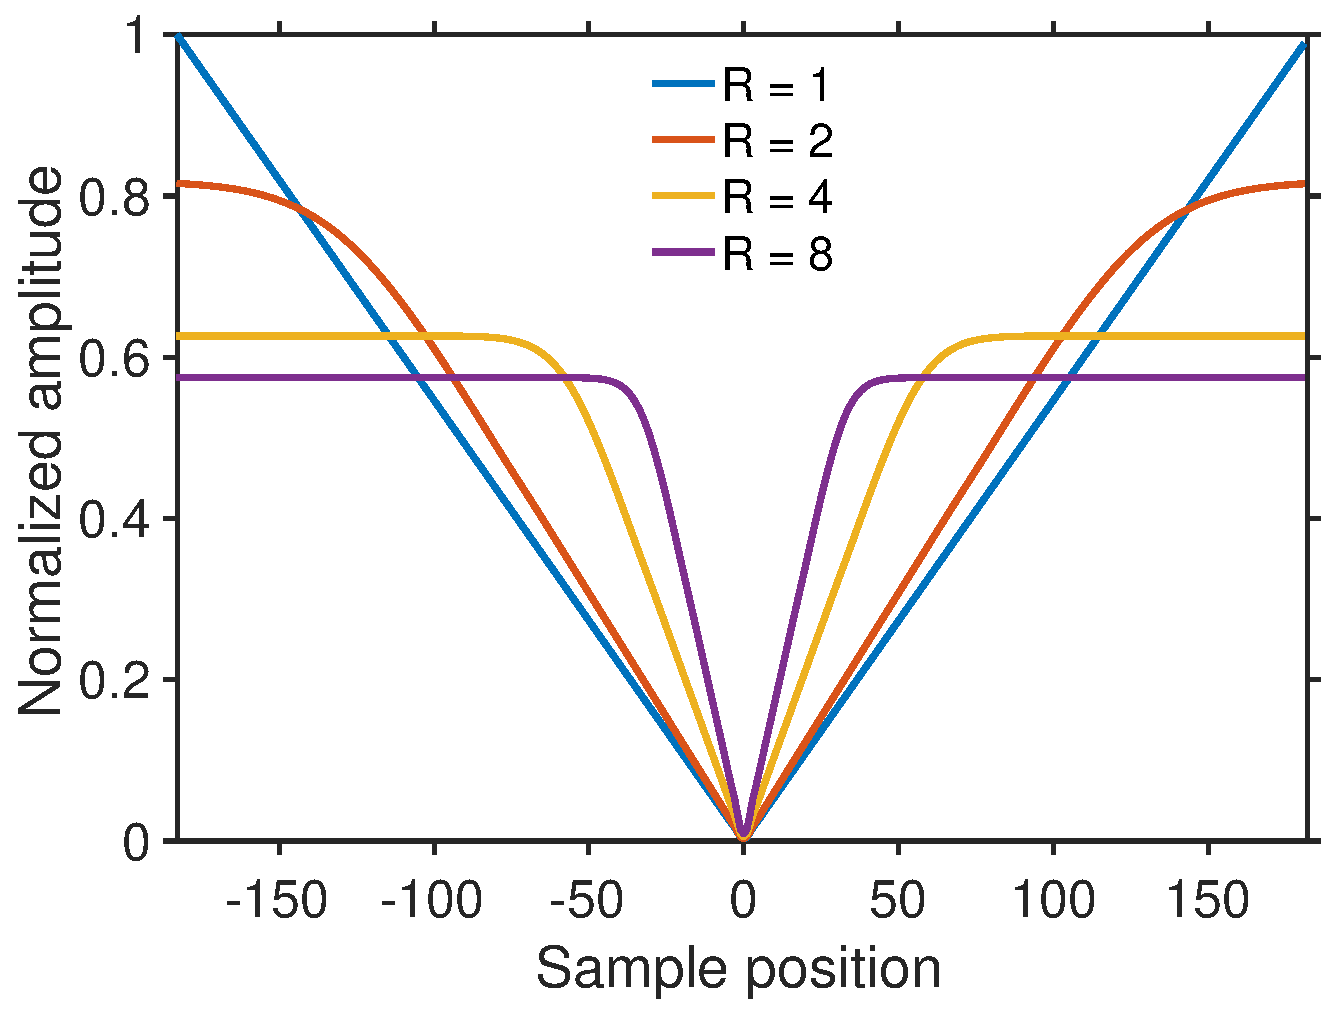
\includegraphics[width=0.65\textwidth]{dcf_pipe}
\caption{Optimized k-space density weighting filters, for a range of undersampling factors, calculated using iterative gridding of the sampling trajectory.}
    \label{fig:pipe}
\end{figure}

\sect{Image reconstruction}
To go from k-space to image space, the Fourier transform is used. However, direct reconstruction of images requires that the sample points are equidistant and that the Nyquist-Shannon sampling theorem is fulfilled in every part of k-space. Violating the Nyquist-Shannon will result in aliasing artifacts. In Cartesian imaging, the aliasing artifacts manifest as ``fold-over'' artifacts where parts of the images is folded back onto itself. The sampling theorem can also be violated on purpose in order to acquire the image faster. By exploiting the variation in spatial sensitivity, \emph{parallel imaging} methods can be used to undo the aliasing, either directly in k-space using GRAPPA \cite{Griswold2002} and SPIRiT \cite{Lustig2010}, or in the image using SENSE \cite{Pruessmann1999}. Many of these methods can be applied to non-Cartesian sampling as well \cite{Wright2014}, such as Radial-GRAPPA \cite{Seiberlich2008, Seiberlich2011} and CG-SENSE \cite{Pruessmann2001}.

\sect{Phase~contrast MRI}
Phase~contrast MRI can be seen as an extension of flow compensation. In MRI, motion is related to phase. 
Phase~contrast~MRI~\cite{Moran1982, Moran1985} measures the velocity of moving spins by making use of the fact that MRI is an inherently phase-sensitive measurement method. The acquired phase due to a static spin with a gradient $G(t)$ is linearly dependent to the 0th gradient moment
\begin{equation}
    M_0 = \gamma \int_0^\tau G(t)\,\dif t
\end{equation}
whereas the phase acquired by spin moving with a constant velocity is dependent on both the 0th the 1st gradient moment,
\begin{equation}
    M_1 = \gamma \int_0^\tau G(t)t\,\dif t. 
\end{equation}
A spin moving with a velocity $v$ will therefore acquire the phase
$\phi = M_0 + v\, M_1$. A phase~contrast image is created by acquiring images encoded with two different $M_1$ values at the echo, encoding A and encoding B \cite{VanDijk1984,Bryant1984}. By subtracting encoding A and B, only the phase due to moving spins is left. In analogy to how the frequency encoding was described in k-space, we can also speak of a velocity k-space value
\begin{equation}
    k_v = \gamma M_1
\end{equation}
An important parameter in phase~contrast MRI is the velocity encoding strength, VENC, which is defined as
\begin{equation}
    \textrm{VENC} = \frac{\pi}{k_v}
\end{equation}
Flow with velocity $\pm$VENC will acquire a phase of $\pm\pi$, whereas higher velocities will experience aliasing, see Figure~\ref{fig:venc}.
\begin{figure}[htbp]
    \centering
    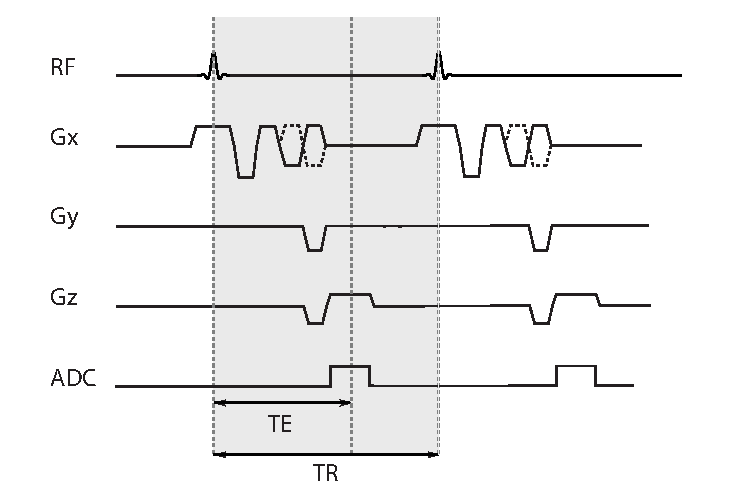
\includegraphics[width=0.75\textwidth]{img/pc3-01.eps}
\caption{The gradient echo pulse sequence diagram from Figure~\ref{fig:gre} has been modified into a phase~contrast pulse sequence with through-slice velocity encoding. Note the addition of flow compensation and bipolar velocity encoding gradients. The solid bipolar gradient pair indicates encoding A, and the dashed gradients indicate encoding B. Note: This is a schematic representation of the pulse sequence diagram, some gradients may not be to scale. Gradient spoilers were omitted for brevity.}
    \label{fig:pc2}
\end{figure}
\begin{figure}[htbp]
    \centering
    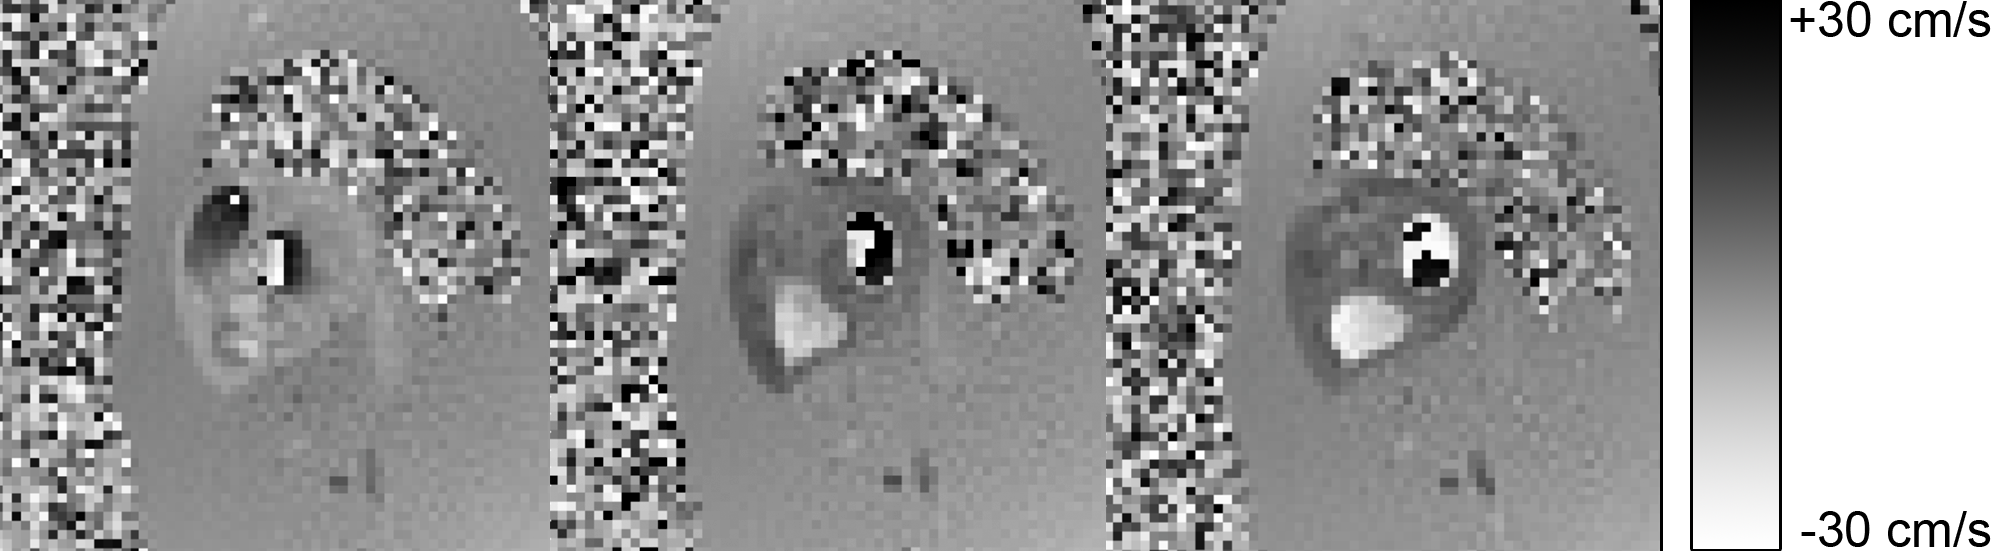
\includegraphics[width=\textwidth]{C14_rev_2_copy.png}
\caption{Illustrative examples of velocity encoded images with VENC = 30 cm/s. Note the aliasing in the left ventricle which is visible as a distinct border between black and white. }
    \label{fig:venc}
\end{figure}

\chap{Cardiovascular Magnetic Resonance Imaging}
The intent of this chapter is to give a brief overview of the history of cardiovascular magnetic resonance (CMR) \Nomenclature{CMR}{Cardiovascular magnetic resonance} imaging and to discuss emerging methods, in particular with respect to self-gated and non-Cartesian methods. 

\sect{A brief overview}
The earliest recorded use of magnetic resonance for probing the function of the heart was Phosphorus-31 NMR spectroscopy of tissue metabolites in ischemic rat hearts~\cite{Hoult1974,Gadian1976,Jacobus1977}. Functional imaging of the heart was introduced with the advent of so-called cine imaging~\cite{Herfkens1983,Lanzer1984,Waterton1985,Sechtem1987a} where the image acquisition was gated using an external electrocardiogram (ECG) \Nomenclature{ECG}{Electrocardiogram} signal. The development of cine methods has enabled accurate measurements of ventricular volumes~\cite{Sechtem1987b} and ejection fractions~\cite{Utz1987}, which are essential functional parameters for determining and diagnosing heart failure. Initial developments in cine imaging used prospective gating and continuous acquisition of one k-space line per heartbeat. This allowed for a very high temporal resolution, but it meant that the acquisition time had to be adapted to the shortest RR-interval. In order not to run into the next heartbeat, the last part of diastole was discarded. With the introduction of the FASTCARD method~\cite{Foo1995}, several lines were acquired repeatedly during the same heartbeat. Using retrospective sorting of the images, it was then possible to cover the entire cardiac cycle, even though there were variations in RR-intervals~\cite{Lenz1989}. To further improve the precision, non-linear stretching of the cardiac cycle has been proposed based on empirical observations of the duration of systole and diastole, respectively~\cite{Feinstein1997}. The continued improvement of the cine imaging techniques means that CMR has developed into a highly accurate method for quantification of cardiac function~\cite{VanDerGeest1999}, and is now considered the non-invasive reference standard~\cite{Pennell2004} for quantifying ventricular volumes, ejection fraction and myocardial mass~\cite{Kramer2020}.

\sect{Free breathing}
The inherent motion sensitivity of cardiac MRI will often require the patient to hold their breath. The heart is resting directly on top of the diaphragm, meaning that breathing motion will change the position of the heart, resulting in motion artifacts. A clinical CMR exam will typically require the patient to hold their breath repeatedly and for extended periods. This precludes the very sickest populations, as cardiovascular disease is often associated with dyspnea. Because of this, it is desirable to acquire images during free breathing.

The earliest example of free-breathing cardiac MRI in the literature refers to measurements of cardiac output in mice, where free-breathing imaging was compared to controlled mechanical ventilation~\cite{Whalen1991}. Prospective navigator gating has been suggested as a viable method for free-breathing coronary angiography~\cite{Danias1997}. By placing exciting a spatially-selective excitation~\cite{Pauly1989} over the liver dome~\cite{McConnell1997}, the acquisition could be triggered or gated according to the respiratory position. An alternative method is to use an external pressure-sensing bellow that can be strapped to the chest or abdomen of the patient to detect respiration, that then can be used similar to a navigator~\cite{Santelli2011}. A potential drawback of using a respiratory bellow is the inherent phase shift between the diaphragmatic position and the abdominal height~\cite{Pengelly1979}. An example of this phase shift can be observed in Figure~\ref{fig:pca_resp}.

\sect{Self-gating}
Conventionally, cine imaging will require an external signal, such as an ECG-signal from the patient ECG to gate or trigger the signal. By a broader definition, a navigator could also be considered an external signal, as it requires setup and planning separate from the imaging sequence. The purpose of self-gating is to derive one or several of these external signals from the data itself~\cite{Larson2004}. As the ECG is typically required for many of the imaging sequences, the most common method has been to use respiratory self-gating to enable free-breathing~\cite{Larson2005}, but methods combining cardiac and respiratory self-gating have also been suggested~\cite{Larson2003:RSNA, DiSopra2019}.

Methods for self-gating can mostly be divided into methods based on image metrics~\cite{McGee2000,Manduca2000}, or methods deriving the motion signal from the raw k-space. Methods that derive motion from k-space usually consider the k-space center signal~\cite{Buehrer2008}, but it is also common to use a single k-space line as an image projection from which motion can be derived~\cite{Pang2014}. Image-based self-gating is often based on reconstructing a real-time image series\cite{Riederer1988, Nayak2004}, from which motion can be estimated, either by simply registering images together~\cite{Kellman2009, Hansen2012, Xue2013}, or by placing an ROI where respiratory or cardiac motion can be observed, such as on the interface between the liver dome and the lung, or in the myocardium of the heart~\cite{Paul2015}.

\begin{figure}
    \centering
    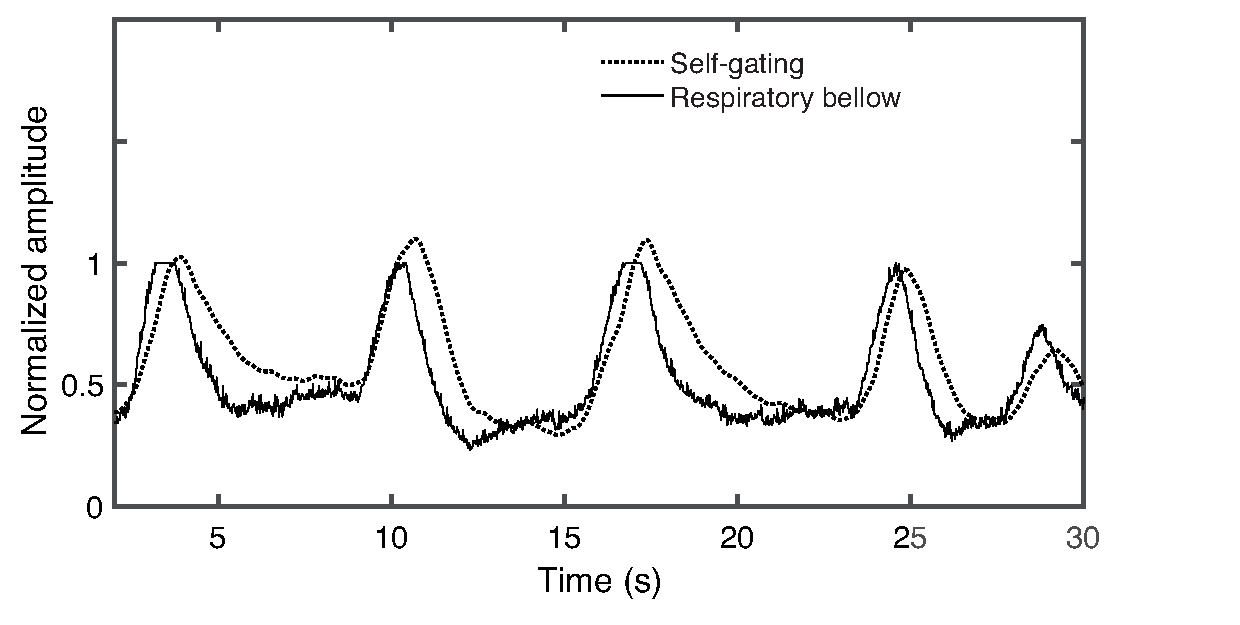
\includegraphics[width=0.75\textwidth]{pca_resp}
    \caption{An example of respiratory motion as detected by a respiratory bellow strapped the patient's abdomen, to record pressure changes due to respiration (solid line). Overlaid is a self-gating signal calculated using principal component analysis of the k-space center (dashed line). }
    \label{fig:pca_resp}
\end{figure}

\begin{figure}
    \centering
    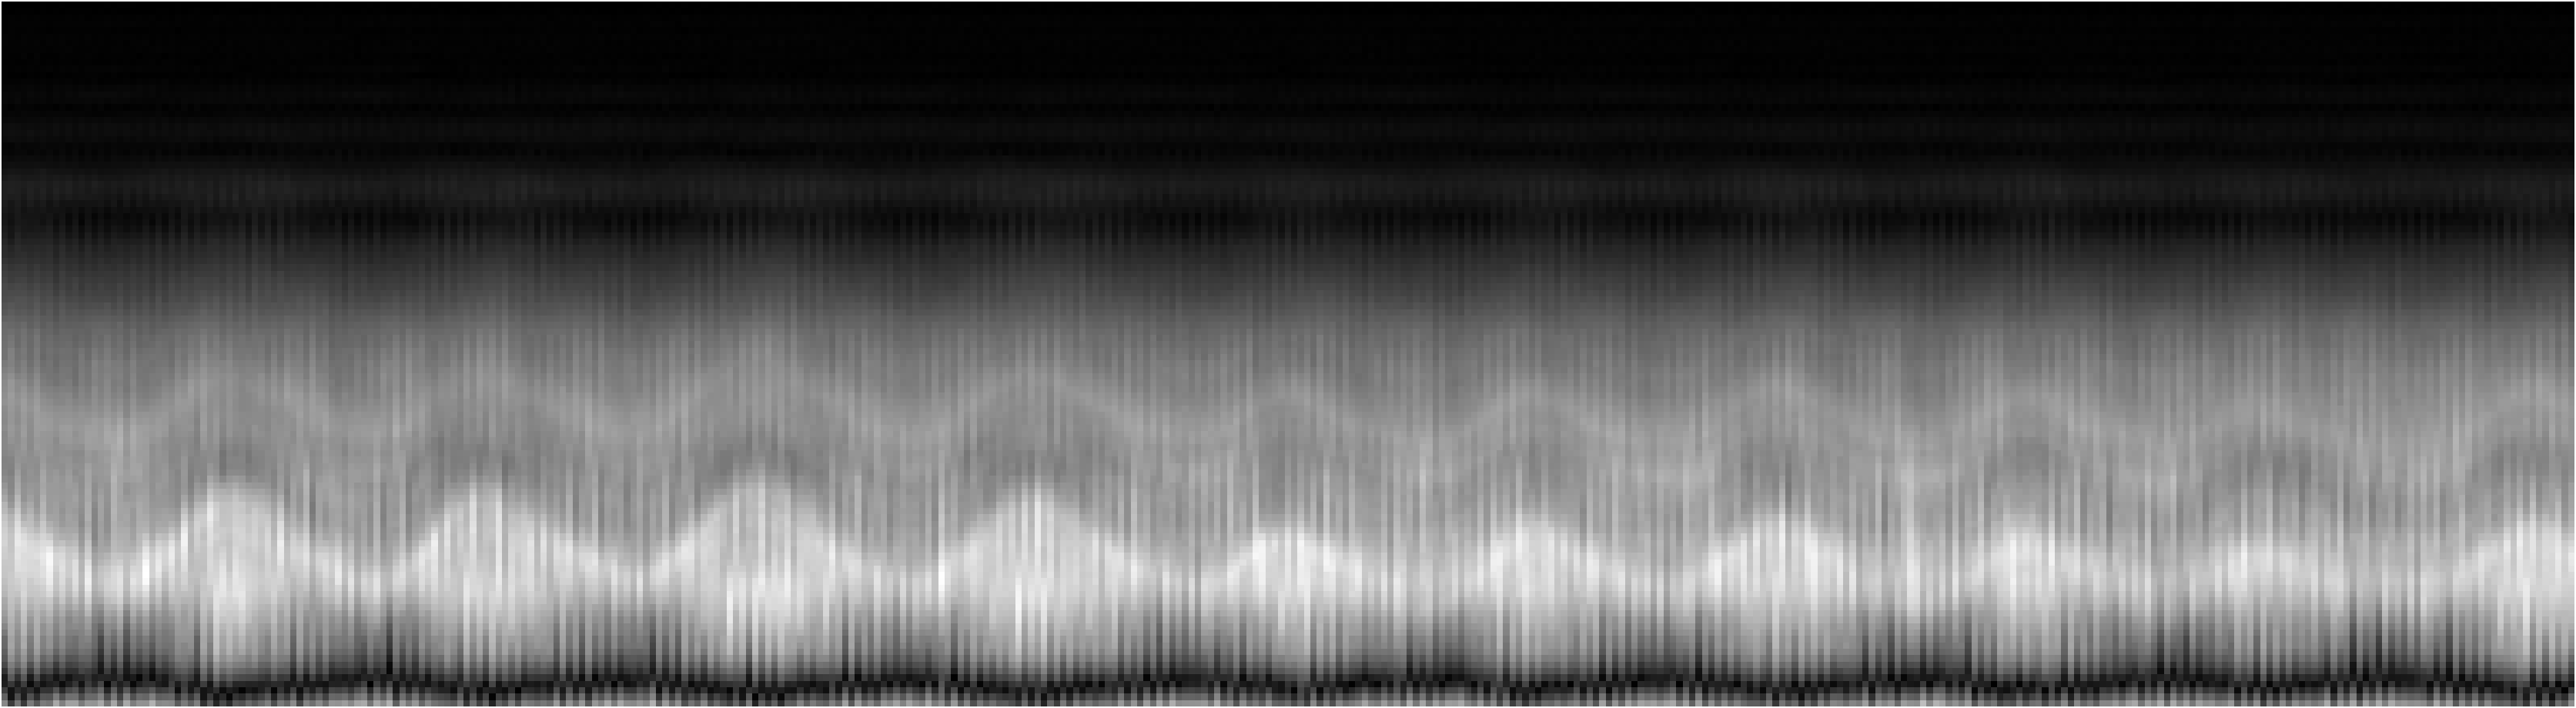
\includegraphics[width=\textwidth]{proj_nav.png}
    \caption{An example of respiratory motion as detected by a projection navigator. }
    \label{fig:proj_resp}
\end{figure}

An example of projection-based self-gating has been combined with the golden-angle by interleaving the readout with a spoke measured in the same direction, with a suitable frequency. This can be done both in 2D~\cite{Kramer2014} and 3D~\cite{Pang2014}.

%\sect{Tissue phase-mapping}
%In a previous section, the phase-contrast method was discussed in the context of measuring flow. However, phase contrast is not limited to flow measurements, and can also be used for tissue velocity measurements~\cite{Paelinck2005}. Tissue velocities are routinely used in Doppler echocardiography as a surrogate measure of left ventricular filling pressures and is a key factor in assessing Diastolic function together with transmitral blood flow velocities~\cite{Silbiger2019}. Tissue-phase contrast have previously been combined with the golden-angle profile ordering~\cite{Paul2016} with image-based self-navigation~\cite{Paul2016b}.
\chap{The Golden Angle}
This chapter is intended to give the reader a brief introduction to the golden ratio and its related mathematical concepts, followed by a brief overview of previous research in MRI with the golden-angle. Finally, a description of the novel methods developed as part of this thesis is presented.

\sect{The golden ratio}
If the ratio between two numbers, $a > b$, is equal to the ratio between the largest of the two and the sum of both, the ratio is called the golden ratio. This can be described as
\begin{equation}
    \label{eq:golden}
    \frac{a}{b} = \frac{a+b}{a} = \varphi
\end{equation}
and
\begin{equation}
    \label{eq:golden2}
    \frac{a+b}{a} = 1 + \frac{b}{a} =
    1 + \frac{1}{a/b}
\end{equation}
Combining Eq.~\ref{eq:golden} and \ref{eq:golden2} yields
\begin{equation}
    \label{eq:golden3}
    \varphi =
    1 + \frac{1}{\varphi}
\end{equation}
The golden ratio $\varphi$ has a few interesting properties. We sometime want to consider its conjugate
\begin{equation}
    \label{eq:conjugate_golden}
    \phi = \frac{1}{\varphi} = 1 - \varphi
\end{equation}
This kind of recursive formula is know as a continued fraction. On a general form, a continued fraction can be written as
\begin{equation}
    \label{eq:contf}
    a + \frac{1}{b + \frac{1}{c + ...}}
\end{equation}
where $a,b,c,...$ are known as partial quotients. An infinite continued fraction can be approximated by its convergents, i.e. what is left i the the recursion is stopped at any given point. If we write the 4 first convergent fractions on simplified form, we end up with
\begin{equation}
\label{eq:quotients}
a, \frac{1+ab}{b}, \frac{a+(1+ab)c}{1+bc}, \frac{1+ab+(a+(1+ab)c)d}{b+(1+bc)d}
\end{equation}
From Eq.\ref{eq:golden3} it's clear that $a = b = c = d = ... = 1$. Substitution yields
\begin{equation}
\label{eq:quotients2}
\frac{1}{1}, \frac{2}{1}, \frac{3}{2}, \frac{5}{3}
\end{equation}
Keeping on in a similar fashion will yield
\begin{equation}
\label{eq:quotients3}
\frac{5}{3}, \frac{8}{5}, \frac{13}{8}
\end{equation}
from Eq.~\ref{eq:quotients2} and \ref{eq:quotients3} we can see that the rational estimation of the golden ratio is in fact the fraction of two successive Fibonacci numbers. By taking the limit of the ratio of successive Fibonacci numbers at infinity we arrive at the golden ratio
\begin{equation}
    \lim_{n\to\infty} = \frac{F_n}{F_{n+1}} = \phi
    \label{eq:limit0}
\end{equation}
where $F_n$ denotes the nth Fibonacci number.

\sect{The golden angles}
There exist several ways to calculate an angle based on the golden ratio. Perhaps the most straight-forward would be to calculate the angle which divides the circle in two parts, where the ratio of the two central angles is the golden ratio
\begin{equation}
360^\circ \cdot \phi = 222.49^\circ  
\end{equation}
\begin{equation}
360^\circ \cdot (1 - \phi) = 137.51^\circ  
\label{eq:large_golden}
\end{equation}
However, it could be useful to only divide the half-circle, resulting in
\begin{equation}
\label{eq:large_ga}   
180^\circ \cdot \phi = 111.25^\circ  
\end{equation}
\begin{equation}
\label{eq:small_ga}
180^\circ \cdot (1 - \phi) = 68.754^\circ  
\end{equation}
Out of these four angles, Eq.~\ref{eq:large_ga} is the golden angle commonly used in MRI~\cite{Winkelmann2007}, whereas the angle defined by Eq.~\ref{eq:small_ga} is sometimes referred to as the small golden angle.

\sect{Multidimensional golden means}
The concept of the golden ratio can also be extended to higher dimensions~\cite{Anderson1993}. Two so called multidimensional golden means $\phi_1 = 0.4656$ and $\phi_2 = 0.6823$ are commonly used. The inverse $1/\phi_2 = 1.4656$ is the fourth smallest of the Pisot-numbers~\cite{Berestovskii2007}, and is sometimes known as the ``super-golden ratio''. It's has been proposed to enable three-dimensional golden-angle imaging~\cite{Chan2009, Trotier2015, Holst2017, Schrauben2020} by mapping the two golden-angles to a two-dimensional unit square
\begin{equation}
    x = \textrm{mod}(m\psi_1,1), y = \textrm{mod}(m\psi_2,1)
    \label{eq:double_golden_square}
\end{equation}
followed by a equal-area mapping of the unit square to a hemisphere
\begin{equation}
    \alpha = 2\pi\cdot x, \beta = \cos^{-1}(y)
\end{equation}
where $\alpha$ is the azimuthal angle and $\beta$ the the polar angle~\cite{Chan2009}.

\sect{Generalized golden angles}

\subsect{Pseudo-golden angles}
The golden-angle is approximately optimal for an arbitrary number of angles, as each succeeding angle of the series divides one of the largest gaps by the golden ratio. However, the number of readout lines are not always unknown at the beginning of the acquisition. Therefore, it would sometimes be useful to adapt the angle to be optimal for a specific number of spokes. This can be achieved in one of two ways. Either, the interval to be measured ($\pi$ or $2\pi$) is divided by a given number of lines, resulting in a so-called linear radial ordering, or by calculating the ``pseudo golden angle'' for the given number of lines~\cite{Svedin2018}.

\subsect{An existing generalization in 2D}
By restating eq.~\ref{eq:golden3}
\begin{equation}
    \phi = \frac{1}{1 - 1 + \frac{1}{\varphi}}
\end{equation}
together with eq.~\ref{eq:conjugate_golden} we note that
\begin{equation}
    1 - \phi = \frac{1}{2 - 1 + \frac{1}{\varphi}}
\end{equation}

It turns out that there exists an infinite series of ratios that have approximately golden properties~\cite{Wundrak2015}. The Nth generalized conjugate golden ratio can be derived through a simple geometric construction
\begin{equation}
\label{eq:general}
    \phi^N = \frac{1}{N-1+\frac{1}{\varphi}}
\end{equation}

This can be seen as a generalized Fibonacci series, $G^N(n+2) = G^N(n+1) + G^N(n)$, for $n \leq 0$ with initial conditions $G^N(0) = 0, G^N(1) = 1, G^N(2)$. By taking the limit of the ratio of the series as $n$ approaches infinity
\begin{equation}
    \lim_{n\to\infty} = \frac{G_n^1}{G_{n+1}^N} = \phi^N
    \label{eq:limit}
\end{equation}

By combining Eq.~\ref{eq:golden3} and Eq.~\ref{eq:general} it is evident that this is a continued fraction where all partial quotients except the first is one, meaning that regardless of N, all of these generalized golden means will be approximately as hard to estimate as a fraction of rational numbers as the original golden ratio.

\subsect{A novel generalization in 3D}
In this thesis, a novel generalization of the double golden angles was proposed, based on a similar construction as in the two-dimensional case.

It is based on the observation that, similar to Eq.~\ref{eq:limit}, the double golden angles can be constructed through a similar generalized Fibonacci series, $H^N(n+3) = H^N(n+2) + H^N(n)$ for $n \leq 0$ with initial conditions $H^N(0) = 0, H^N(1) = 1, H^N(2) = N$ at the limit

\begin{equation}
        \lim_{n\to\infty} = \frac{H_n^1}{H_{n+1}^N} = \phi^N_1 \quad \textrm{and} \quad \lim_{n\to\infty} = \frac{H_n^1}{H_{n+2}^N} = \phi^N_2
\end{equation}

will yield the original multidimensional golden means for N = 1, and for $N \geq 2$ will generate golden means with similar properties to the original golden means.

A geometric construction, similar to Eq.~\ref{eq:general} is also possible in 3D, and can be describes as
\begin{equation}
    \psi^N_2 =  \frac{1}{N - 1 + \frac{1}{\psi_2}} \quad \textrm{and} \quad \psi^N_1 = \frac{\psi^N_2}{1 + \psi_1}
\end{equation}
where $\psi_1$ and $\psi_2$ are the two original golden means. This is further discussed in Study II.

\sect{Golden angle in the literature}
The golden angle have found many uses within the field of MRI since the seminal paper was published in 2007~\cite{Winkelmann2007}. Many early adaptations were focused on dynamic contrast-enhanced (DCE) \Nomenclature{DCE}{Dynamic contrast enhancement} of chest and abdominal lesions~\cite{Lin2008}, breast MRI~\cite{Chan2009} and angiography~\cite{Prieto2010}. However, the golden-angle has found uses in many diverse areas, such as T1-mapping~\cite{Ehses2013, Tran-Gia2015} and diffusion weighted imaging~\cite{Seo2014}. In the field of cardiac MRI, the golden angle has been used for tissue phase mapping~\cite{Paul2016, Paul2016b}, imaging of arrhythmia~\cite{Contijoch2017}, determining pressure-volume loops~\cite{Witschey2014}, myocardial perfusion imaging~\cite{Sharif2014}, and measurement of respiratory induced variations in left-ventricular volumes~\cite{Holst2017, Holst2018, Holst2019}.

Arguably, the most successful method is Golden Angle Radial Sparse Parallel MRI (GRASP) \Nomenclature{GRASP}{Golden Angle Radial Sparse Parallel MRI}. It is a framework for dynamic contrast enhanced liver imaging~\cite{Feng2014}, which has been expanded with self-gating capabilities to the extra-dimensional GRASP (XD-GRASP) framework~\cite{Feng2015} for resolving multiple, and arbitrary temporal dimensions at once, such cardiac time and respiratory time~\cite{Feng2018}. The XD-GRASP formulation is based on the idea of a Sparse-SENSE~\cite{Feng2013}, which is based on an iterative SENSE reconstruction~\cite{Pruessmann2001} that is regularized by multiple sparse constraints~\cite{Lustig2007}. The general formulation can be described as a minimization problem on the form

 \begin{equation}\label{eq:argmin}
	\hat{\textbf{x}} = \argmin_{\textbf{x}} \|\textbf{y} - \textbf{E}\textbf{x} \|^2_2 + \lambda_1 \|\Psi_1\textbf{x}\|_1 + \lambda_2 \|\Psi_2\textbf{x}\|_1 + \dots + \lambda_N \|\Psi_N\textbf{x}\|_1
\end{equation}

where $\textbf{x}$ is the image, $\textbf{y}$ is the measured data, $\textbf{E}$ is the SENSE operator which includes the gridding step, Fourier transform and the coil sensitivities~\cite{Pruessmann2001}, $\Psi_N$ is the sparsifying transform in the Nth dimension~\cite{Lustig2007} and $\lambda_N$ controls the amount of regularization in the Nth dimension.

Another recent development making use of the golden-angle is the so-called MR multitasking method~\cite{Christodoulou2018, Shaw2019}, which uses a golden-angle readout with an integrated one-dimensional projection navigator and low-rank tensor decomposition to enable multiple simultaneous parameter mapping.

Other golden angle based methods may use the golden angle indirectly, e.g., for rotating spiral interleaves by the golden angles, often Eq.~\ref{eq:large_golden} to cover a full $360^\circ$ is commonly used~\cite{Kim2011}, or the ``spiral phyllotaxis'' method~\cite{Piccini2011, Piccini2017, Coppo2015}, which is a 3D-radial method based which traces Fibonacci spirals on the surface of the trajectory sphere, and where each interleave is rotated by the golden angle. The spiral phyllotaxis method has been used to enable fully respiratory and cardiac self-gated acquisitions~\cite{DiSopra2019}.

\sect{SWIG-PC}
In Study III, a novel phase-contrast pulse sequence was developed using a sector-wise golden-angle profile ordering~\cite{Han2016}, symmetric velocity encoding~\cite{Bernstein1992}, and a shared velocity encoding reconstruction~\cite{Bernstein1994, Lin2012}, to effectively double the number of reconstructed image frames. We decided to name this particular sequence ``Sector-wise golden-angle phase contrast'' or SWIG-PC for short. 

The golden-section division is performed according to the formula
\begin{equation}
    \phi_{n+1} = \textrm{mod} \left[ \left( \phi_n + \frac{\pi}{N} \cdot \frac{\sqrt{5}-1}{2} \right), \frac{\pi}{N} \right] + s \cdot \frac{\pi}{N}
\end{equation}
adapted from~\cite{Han2016}, where $s = 0, 1, 2, \dots, N$ denotes the current heartbeat, N is the total heartbeats to acquire and $\phi_n$ the $n$th angle, see Figure~\ref{fig:swig_overview}.

\begin{figure}
    \centering
    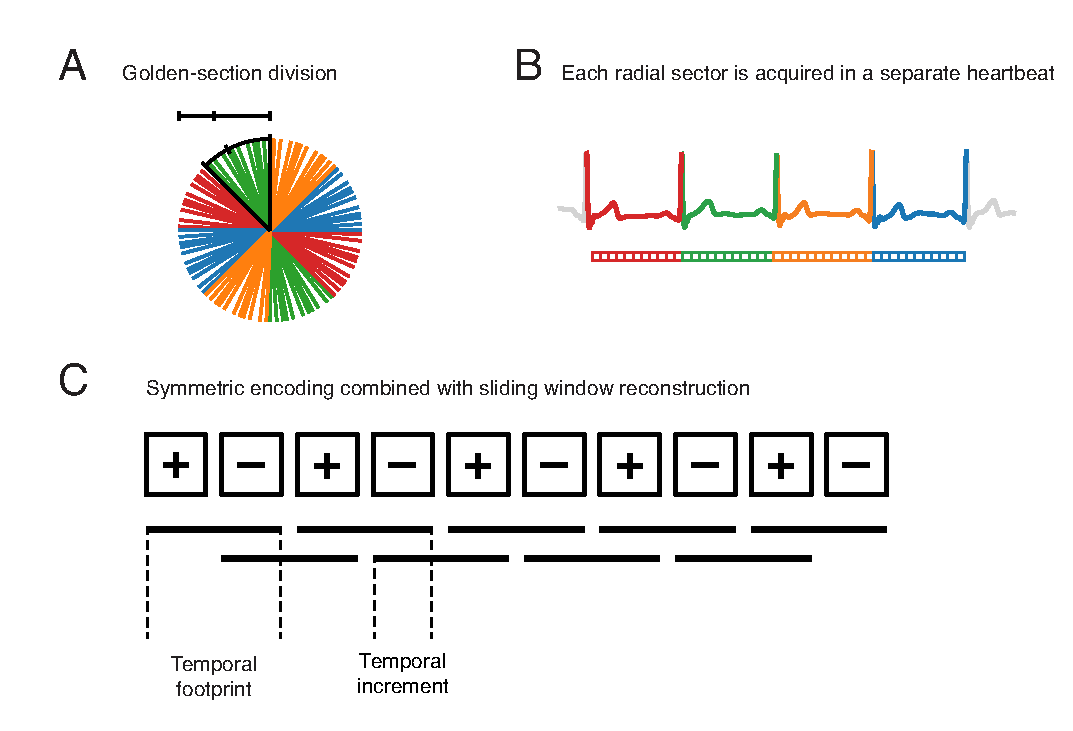
\includegraphics[width=\textwidth]{Figure_1_schematic_description}
    \caption{Schematic description of the SWIG-method. The k-space is sampled sector-wise with golden-section division within a sector of k-space (A). On each heartbeat, the acquisition moves to a new sector (B). Upon reconstruction, shared velocity encoding is used to double the reconstruction frames by performing phase subtraction between alternating positively- and negatively velocity encoded images. Reproduced with permission from~\cite{Fyrdahl2020}. (Licensed under CC BY 4.0) }
    \label{fig:swig_overview}
\end{figure}

The sector-wise golden angle profile ordering was combined with a TR-interleaved symmetric velocity encoding, to enable high temporal resolution phase contrast. This was applied to measuring diastolic dysfunction parameters in \textbf{Study II}.

\sect{3D-SWIG}
In Study IV, further development of the SWIG-PC method proposed in Study III was proposed. Instead of using phase contrast, we opted for functional imaging using bSSFP contrast. We decided to call the novel development ``3D Sector-wise golden angle'' or 3D-SWIG, for short.

Instead of mapping angles to a circle sector, as in SWIG-PC, polar coordinates were mapped to solid angles on a hemisphere. To enable a low distorting, uniform mapping, a method for constructing spherical grids~\cite{Rosca2011}, adapted to map coordinates from a cube to a sphere, see Figure~\ref{fig:mapping}. The resultant transform can be described as

\begin{equation}
    X' = x \cdot \sqrt{1-\frac{y^2}{2}-\frac{z^2}{2}-\frac{y^2z^2}{2}}
\end{equation}
\begin{equation}
    Y' = y \cdot \sqrt{1-\frac{z^2}{2}-\frac{x^2}{2}-\frac{z^2x^2}{2}}
\end{equation}
\begin{equation}
    Z' = z \cdot \sqrt{1-\frac{x^2}{2}-\frac{y^2}{2}-\frac{x^2y^2}{2}}
\end{equation}

Using this proposed mapping, combined with the golden means division of unit squares described in Eq.~\ref{eq:double_golden_square}, but applied for each grid cell, and acquiring one grid cell per heartbeat, as described in the SWIG method, a very uniform k-space uniformity can be achieved after physiological binning. This method was implemented and tested both using numerical simulations, phantom images, and \emph{in vivo} in \textbf{Study IV}.

\begin{figure}
    \centering
    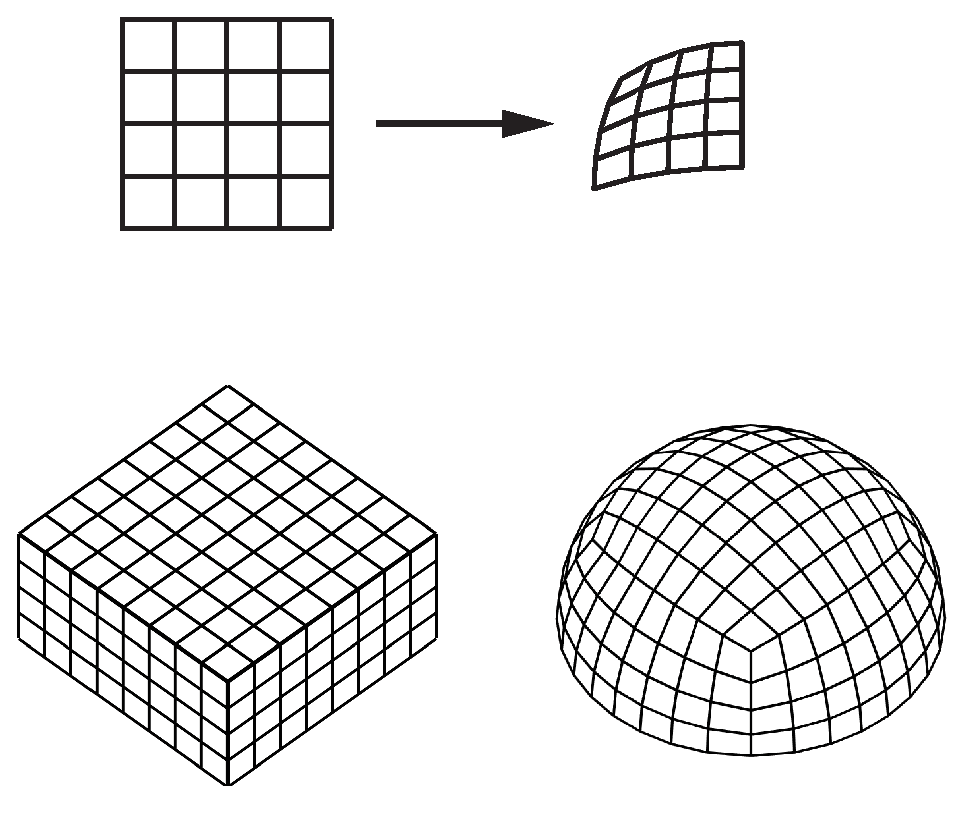
\includegraphics[width=0.65\textwidth]{mapping}
    \caption{A schematic description of the mapping from a rectilinear patch to a patch on the sphere surface (top). The entire mapping from a half-cube to a hemisphere (bottom). }
    \label{fig:mapping}
\end{figure}
\chap{Aims}
The overall aim of this thesis was to explore, evaluate, and develop potential methods using radial imaging. In particular, the golden angle and golden-angle-based sampling were evaluated for increasing the effectiveness of cardiovascular magnetic resonance imaging.

The specific aims for Study I-IV were
\begin{enumerate}[I.]
    \item To develop a methodology for golden angle radial imaging of pulmonary arteries, without breath-holding or intravenous contrast agents, and evaluate the potential improvement in image quality in healthy volunteers and patients with pulmonary embolism. 
    \item To design a generalization of the three-dimensional golden angle radial profile ordering to reduce the eddy current induce image artifacts in bSSFP MRI.
    \item To improve temporal resolution in golden angle radial phase-contrast CMR to enable diastolic dysfunction assessment.
    \item To design a three-dimensional sector-wise golden angle radial profile ordering that enables improved k-space uniformity after ECG binning.
\end{enumerate}
\chap{Materials and methods}
This chapter gives a brief overview of the methods used in the four studies that make up this thesis. Many of the novel concepts have been discussed in previous chapter. The purpose of this chapter is to provide complementary information on how the methods were evaluated. For a complete description, see Studies I-IV.

\sect{Study populations}
 In \textbf{Study I} the method was therefore first tested on 10 healthy volunteers (age $44\pm11$ years, 50\% female), and on two patients (age 27 and 38, both female) which had a confirmed and clinically established diagnosis of pulmonary embolism. Out of the 10 volunteers, 9 were given the same protocol as the patients. However, the last volunteer in the volunteer cohort was given an extended protocol, where the reference method was tested under several conditions other than the normal acquisitions, to isolate respiratory and cardiac motion. This required a motivated volunteer, and would not be feasible in a patient population. \textbf{Study II} was entirely focused on the methodology, and most work was made using numerical simulations and phantom images. One healthy volunteer was recruited (female, 27 years) to evaluate the method \emph{in vivo}. In addition, ECG and respiratory motion signals that were recorded in 8 healthy volunteers to be used in the numerical simulations. \textbf{Study III} was the most clinically oriented study. The purpose of the study was to study functional parameters, so patients from the clinical workflow were included on a consecutive basis. Whereas there was no stratification or other type of attempt to steer the inclusion, the final population comprised a range of different pathologies representative of what can be expected in the clinic. The population was divided into two groups chronologically. The first, smaller group was used to determine suitable parameters for the image acquisition and reconstruction, whereas the second larger group was used to evaluate the method with parameters determined from the first group. The characteristics of the groups are outlined in Table~\ref{table:study3pop}.
\begin{table}[tbp]
\caption{Characteristics of the study population from Study III.}
\begin{center}
\begin{threeparttable}
\begin{tabular}{l c c}
     \mydarkrowcolor~ & \textbf{Pilot study, N = 10} & \textbf{Main population, N = 35}\\
     Age & $64 \pm 10$ years & $56 \pm 16$ years \\
     \myrowcolor Male & 4 (40\%) & 24 (69\%) \\
      Female & 6 (60\%) & 11 (31\%)\\
     \mydarkrowcolor \textbf{Pathology by CMR} & & \\
     Myocarditis & 1 (10\%) & 2 (6\%) \\
     \myrowcolor Pericarditis & 0 (0\%) & 3 (9\%) \\
     Cardiomyopathy & 2 (20\%)& 4 (11\%)\\
     \myrowcolor Acute myocardial ischemia &2 (20\%) & 9 (26\%) \\
     Ischemic heart disease &5 (50\%) & 11 (31\%)\\
     \myrowcolor Valvular pathology & 0 (0\%) & 2 (6\%)\\
     Normal findings & 0 (0\%) & 4 (11\%) \\
     \bottomrule
\end{tabular}
\begin{tablenotes}
\emph{Note:} Continuous variables are given as mean $\pm$ SD.
\end{tablenotes}
\end{threeparttable}
\end{center}
\label{table:study3pop}
\end{table}

\textbf{Study IV} was also focused on method development rather than clinical diagnosis. Three subjects who gave informed consent were included from the clinical workflow, without any particular regard towards clinical referral.

Ethical approval was obtained for all studies, and all participants gave their written, informed consent to participate in the studies.
\sect{Numerical simulations}
\subsect{Study I}
In Study I, numerical simulations were used to estimate the sensitivity of random phase perturbations for Cartesian and radial trajectories, respectively. A numerical phantom was constructed in MATLAB (Mathworks, Natick, MA), depicting a transversal slice of the upper thoracic cavity. Complex noise was added at every time step of the simulation, as well as a random through-plane contribution and intensity modulation in the ascending and descending aorta, to simulate effects due to through-plane flow, see Figure~\ref{fig:numerical}.
\begin{figure}
    \centering
    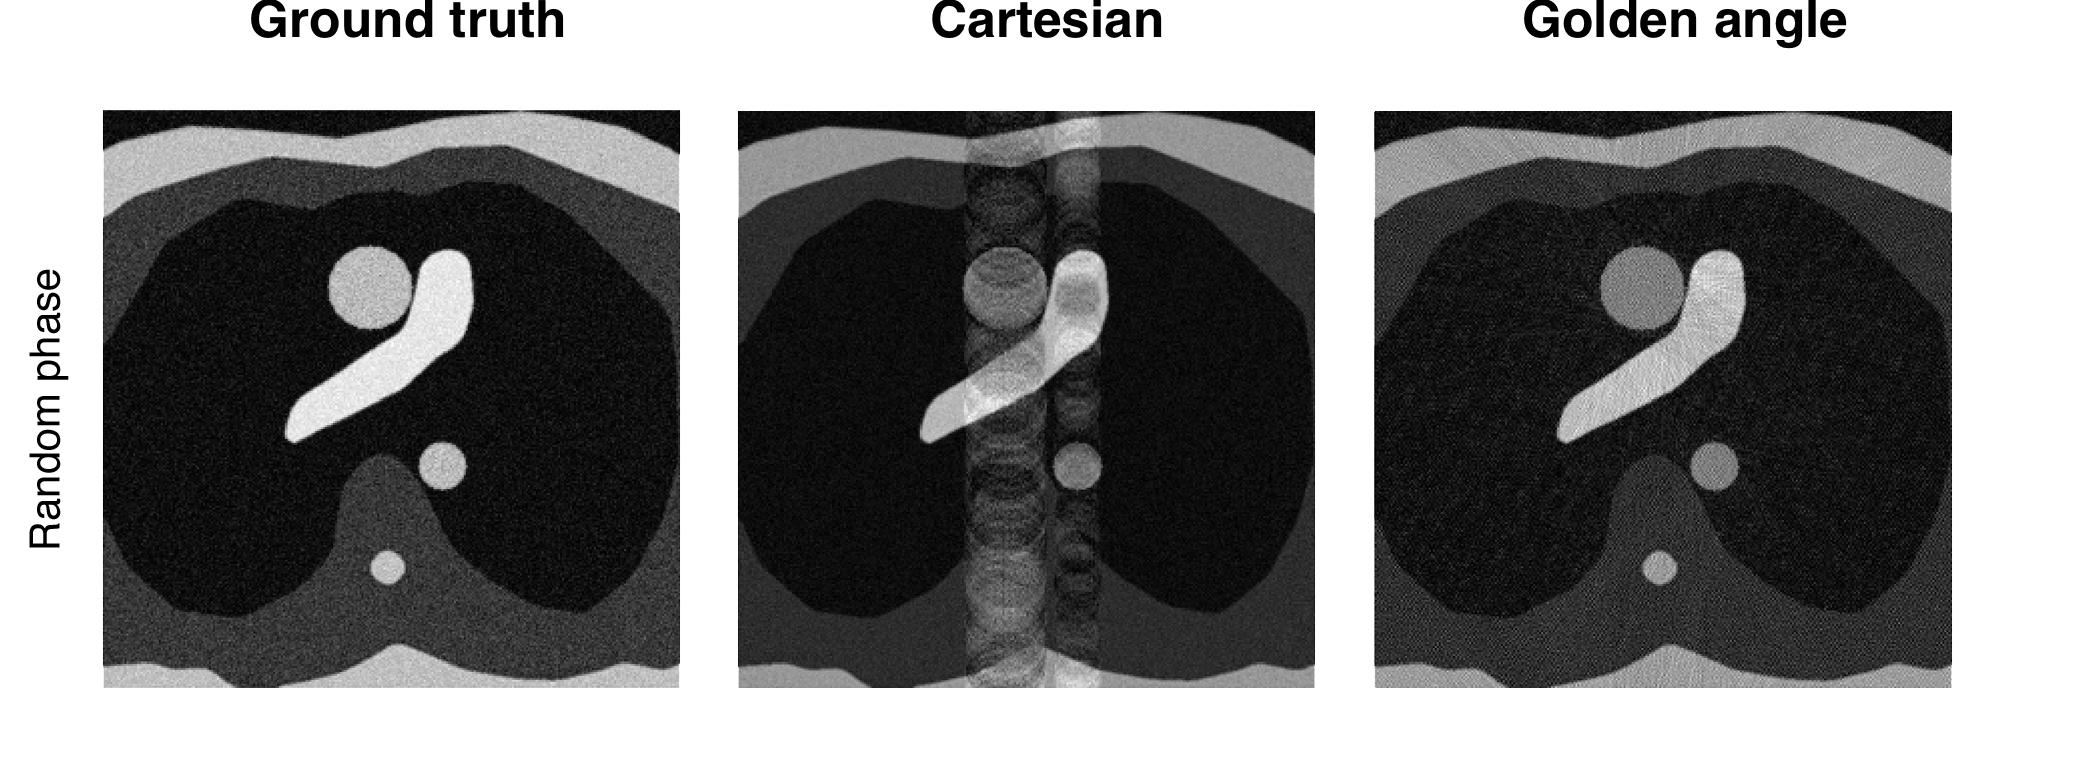
\includegraphics[width=\textwidth]{numerical.png}
    \caption{A numerical simulation of the effects of sampling an image with through-plane phase modulation when using a Cartesian (middle) and radial (left) readout trajectory. Reproduced with permission from~\cite{Fyrdahl2018}. Copyright \copyright~2018 International Society for Magnetic Resonance in Medicine. Published by John Wiley \& Sons Inc.}
    \label{fig:numerical}
\end{figure}
\subsect{Study II}
In Study II, a mathematical theory was proposed as a generalization for three-dimensional golden angles; see previous chapters. To evaluate the proposed generalization, numerical simulations were performed to calculate a clustered-regular-random (CRR) \Nomenclature{CRR}{Clustered Regular Random} value for the generalized profile orderings. CRR was defined as
\begin{equation}
    \textrm{CRR} = 2 \cdot \frac{\sum_{i\ne j}^{P} \textrm{min}(u_{i,j})}{\sqrt{P}}
\end{equation}
where P was the total number of sampling points and $u_{i,j}$ was the distance between sampling points $i$ and $j$. The mean angle between successive readout spokes was calculated as a measure of the gradient switching.

\subsect{Study III}
In Study III, numerical simulations of the point-spread function (PSF) \Nomenclature{PSF}{Point spread function} was performed. The PSF can be defined as the effect from voxel $i$ on all other voxels. The PSF due to voxel $i$ in voxel $j$ can be calculated as
\begin{equation}
    \textrm{PSF}(i,j) = e_j^*F^*e_i
    \label{eq:psf}
\end{equation}
where $e_i$ is a zero-vector with a single unitary value on the $i$th position and F is the encoding matrix, which in this case was the non-uniform Fourier operator.

The PSF was calculated for all voxels in an image frame, using the conventional golden-angle profile ordering and the proposed SWIG profile ordering. The maximum value and the sum-of-squares value of the PSF was calculated at concentric distances from the k-space center to classify the PSF at a distance from the k-space center.
\subsect{Study IV}
In Study IV, an extension of the profile ordering from Study III was proposed in 3D. The profile ordering was calculated for 12, 48 and 192 sectors, and the PSF was classified for each profile ordering, as described in Eq.~\ref{eq:psf}. Physiological binning was calculated for the 3 subjects, for both the conventional golden-angle profile ordering and the 3D-SWIG profile ordering, where 20 cardiac bins were calculated for each subject. Spherical Voronoi diagrams were calculated for each of the bins, and the mean Voronoi area was used as a metric of k-space uniformity.

\sect{Image acquisition and analysis}
All images were acquired on two clinical MRI systems from the vendor Siemens. One system had a field strength of 1.5 Tesla (Aera, Siemens Healthcare, Erlangen, Germany) and the other had a field strength of 3 Tesla (Skyra, Siemens Healthcare, Erlangen, Germany). The scanner software version on all scanners were the same for all studies included in this thesis (syngo MR E11A, Siemens Healthcare, Erlangen, Germany). The signal reception was performed with nearly identical surface coil arrays for both field strengths. One 18 channel general purpose ``body'' receive-only coil (Body 18, Siemens Healthcare, Erlangen, Germany) comprised of 3 rows with 6 coil elements on each row, giving a total of 18 coil array elements and a ``spine'' receive-only coil integrated into the patient table (Spine 32, Siemens Healthcare, Erlangen, Germany) comprising 8 rows with 4 coil elements on each row, giving a total of 32 coil array elements. Both systems were equipped with the same gradient specifications. The maximum gradient amplitude was 45 mT/m and the maximum slew rate was 200 T/m/s.
\subsect{Study I}
The protocol in Study I was designed to compare the novel proposed method to a previously proposed Cartesian protocol, using non-enhanced bSSFP and multiple repetitions of each slice position~\cite{Nyren2017}. Two image series were acquired, one golden-angle radial image series and one Cartesian image series. Both series comprised 70 contiguous slices with 3 mm slice thickness and no slice gap to cover the entire thorax. The sequences were matched as closely as possible, but due to technical limitations, some adjustment had to be made. All sequence parameters are outlined in Table~\ref{table:study1protocol}.
\begin{table}[htbp]
\caption{Sequence parameters from Study I.}
\begin{center}
\begin{threeparttable}
\begin{tabular}{l c c}
     \mydarkrowcolor \textbf{Parameter} & \textbf{Cartesian} & \textbf{Golden-Angle}\\
     TE (ms) & 1.6 & 1.8   \\
     \myrowcolor TR (ms) & 1.8 & 3.6 \\
     Readout lines (N)  & 163 & 1345 \\
     \myrowcolor Parallel imaging method & GRAPPA & SPIRiT \\
     ACS lines (N) & 38 & –– \\
     \myrowcolor Flip angle (deg) & 60 & 60 \\
     Bandwidth (Hz/px) & 1008 & 1008 \\
     \myrowcolor FOV (mm$^2$) & 420 & 420 \\
     Matrix size (px) & 288 & 288 \\
     \myrowcolor Acquired voxel size (mm$^2$) & $2\times2$ & $2\times2$\\
     Reconstructed voxel size (mm$^2$) & $2\times2$ & $2\times2$\\
     \myrowcolor Slice thickness (mm) & 3 & 3\\
    Number of slices (N) & 70 & 70 \\
    \myrowcolor Acq. time per slice (ms) & 522 & 4842 \\
    Total acq. time (s) & 40 & 340 \\
     \bottomrule
\end{tabular}
\begin{tablenotes}
\emph{Note:} ACS = Auto-calibrating signal \Nomenclature{ACS}{Auto-calibrating signal}.
\end{tablenotes}
\end{threeparttable}
\end{center}
\label{table:study1protocol}
\end{table}
From the golden-angle acquisitions, there where two additional data sets created by truncating the long acquisition. These corresponded to an oversampled set, an approximately fully sampled set and one undersampled set. The number of spokes in the oversampled set was chosen as all acquired spokes, the number of spokes in the fully sampled set was chosen as the Fibonacci number closest to a fully sampled acquisition according to the radial Nyquist criterion (i.e. the Nyquist criterion fulfilled at all parts of k-space) and the undersampled set was chosen such that the acquisition time matched that of the Cartesian acquisition. See Table~\ref{table:study1subgroups} for a complete description of the three data sets used for further analysis.
\begin{table}[htbp]
\caption{Description of the subgroups from Study I.}
\begin{center}
\begin{threeparttable}
\begin{tabular}{l c c c}
     \mydarkrowcolor \textbf{Parameter} & \textbf{Oversampled} & \textbf{Fully sampled} & \textbf{Undersampled}\\
     Spokes & 1345 & 610 & 144 \\
     \myrowcolor Cartesian undersampling (R) & 0.2 & 0.5 & 2 \\
     Radial undersampling & 0.33 & 0.74 & 3.1 \\
     \myrowcolor Acq. time per slice (ms) & 4842 & 2196 & 518 \\ 
     Total acq. time (s) & 340 & 150 & 40 \\
     \bottomrule
\end{tabular}
\begin{tablenotes}
\emph{Note:} Cartesian undersampling is the matrix size divided by the number of spokes. Radial undersampling is calculated relative to the Nyquist criterion at the edge of k-space.
\end{tablenotes}
\end{threeparttable}
\end{center}
\label{table:study1subgroups}
\end{table}
The previously described protocol was performed in 10 healthy volunteers, and in 2 patients. In one healthy volunteer, an additional acquisition was performed. In 20 slices covering the right pulmonary artery (RPA) and the left pulmonary artery (LPA). The acquisitions were performed during free-breathing, breath hold (end-expiratory), with ECG-triggering, and with a combination of breath hold and ECG-triggering.
In the patients, the blood-to-blood-clot contrast was measured by delineating blood clots and measuring the signal intensity within the clot. The blood-to-blood-clot-contrast was then calculated as
\begin{equation}
    C_{\textrm{blood,clot}} = \frac{S_{\textrm{blood}} - S_{\textrm{clot}}}{S_{\textrm{blood}}+S_{\textrm{clot}}}.
    \label{eq:bloodclotcontrast}
\end{equation}
The sharpness of pulmonary vessels was calculated using the Deriche algorithm~\cite{Deriche1990} by computing an edge image using a recursive Gaussian filter algorithm, then calculating a line-profile perpendicular to the vessels. The amplitude of the vessel wall in the edge image was used as a metric of the vessel sharpness.

Qualitative analysis of the images was performed using observer scoring, where two experienced radiologists were asked to score the images on a scale from 1 to 5, where a higher score signified better quality than a lower score.

\subsect{Study II}

A prototype 3D-radial bSSFP pulse sequence was modified to allow for sampling with 3D golden-angles. A user-selectable parameter was added to the sequence that allowed the operator to freely select a parameter that controlled the degree of the generalized profile ordering. By increasing the parameter, the mean angle between successive readouts was decreased. For further details on the implementation, see Study II.

Pre-recorded physiological signals (respiration and ECG) from 8 healthy volunteers were used to simulate physiological binning~\cite{Holst2017} and spherical Voronoi diagrams were calculated on the surface of the trajectory sphere. The standard deviation of the Voronoi cell area was used as a measure of the resultant sampling uniformity after the physiological binning was performed.

\subsect{Study III}
In Study III, a novel phase-contrast pulse sequence was proposed to enable high temporal resolution measurements of blood flow and tissue velocities.

In all subjects, a short-axis slice was planned by placing the imaging slice plane at the tip of the mitral valves in systole. Two images were acquired using this planning. One image with VENC = 30 cm/s for myocardial tissue velocities, and one image with VENC = 150 cm/s for transmitral blood flow velocities, see Figure~\ref{fig:swig_planning}.

\begin{figure}[htbp]
    \centering
    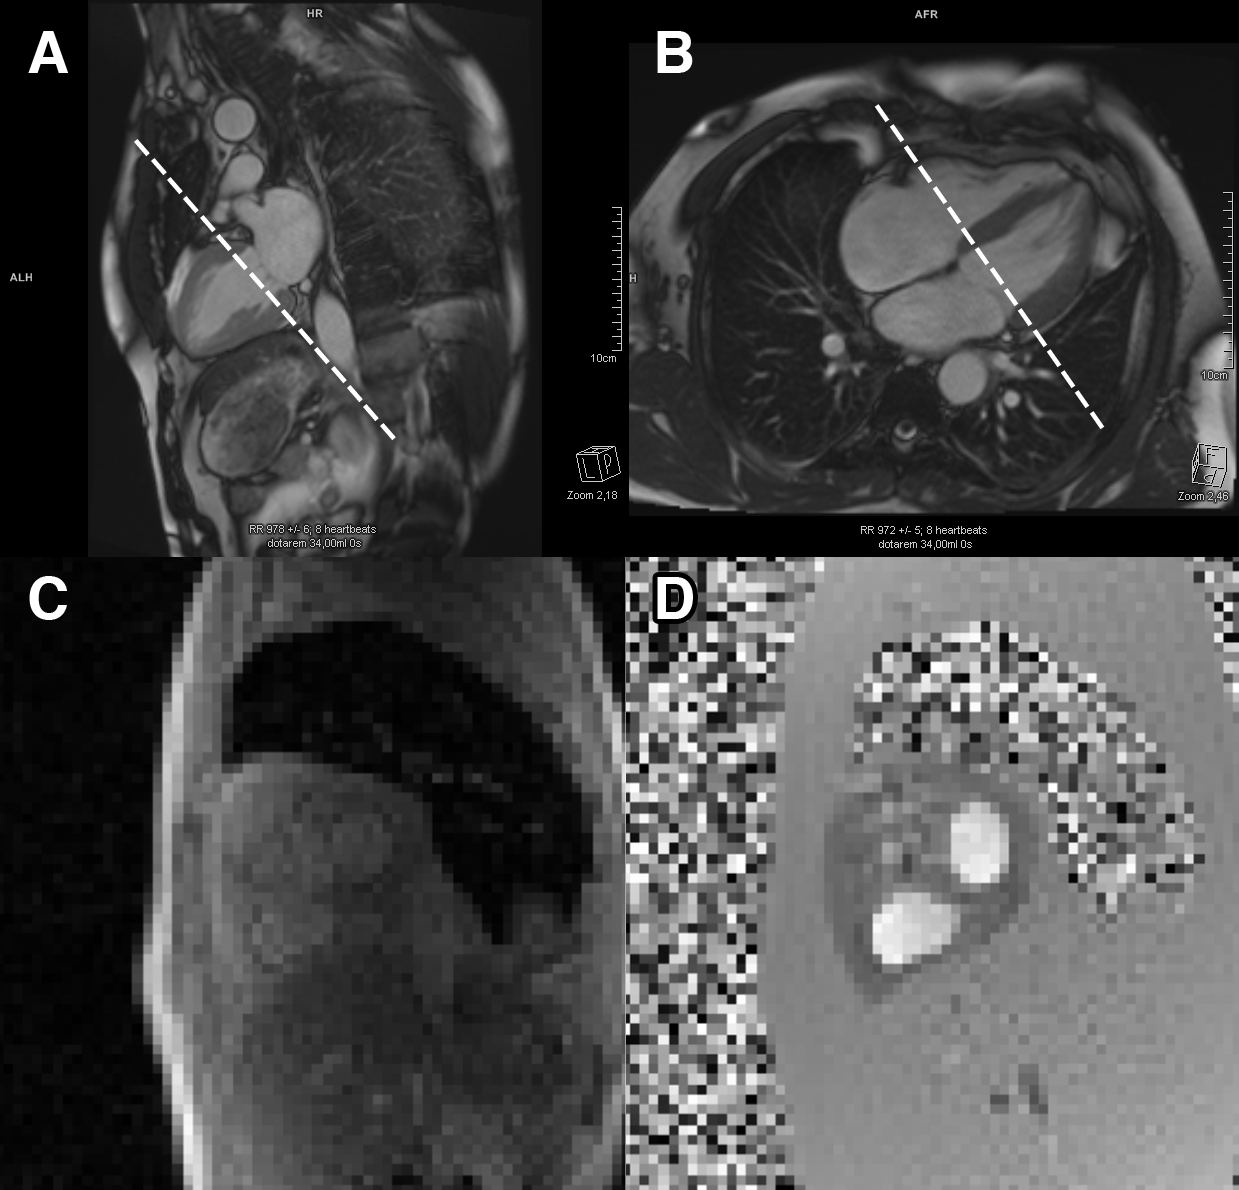
\includegraphics[width=0.75\textwidth]{Figure_2_planning.png}
    \caption{Planning was performed by planning a short-axis slice, indicated by the dashed white line, at the tip of the mitral leaflets in end-systole. The planning is displayed in a 2-chamber orientation (A) and a 4-chamber orientation (B). The resulting images from SWIG pulse sequences are displayed as a magnitude (C) and phase (D) image pair using VENC = 150 cm/s for transmitral blood flow measurements.}
    \label{fig:swig_planning}
\end{figure}

The image analysis was performed in Segment v2.1 R6069 (Medviso AB, Lund, Sweden)~\cite{Heiberg2010} using an in-house developed plugin to enable velocity measurements in a single voxel at the time, see Figure~\ref{fig:segment_gui}. Prior to analysis, quadratic static tissue compensation was performed, as well as semi-automatic phase unwrapping in the few cases where this was necessary.

\begin{figure}[htbp]
    \centering
    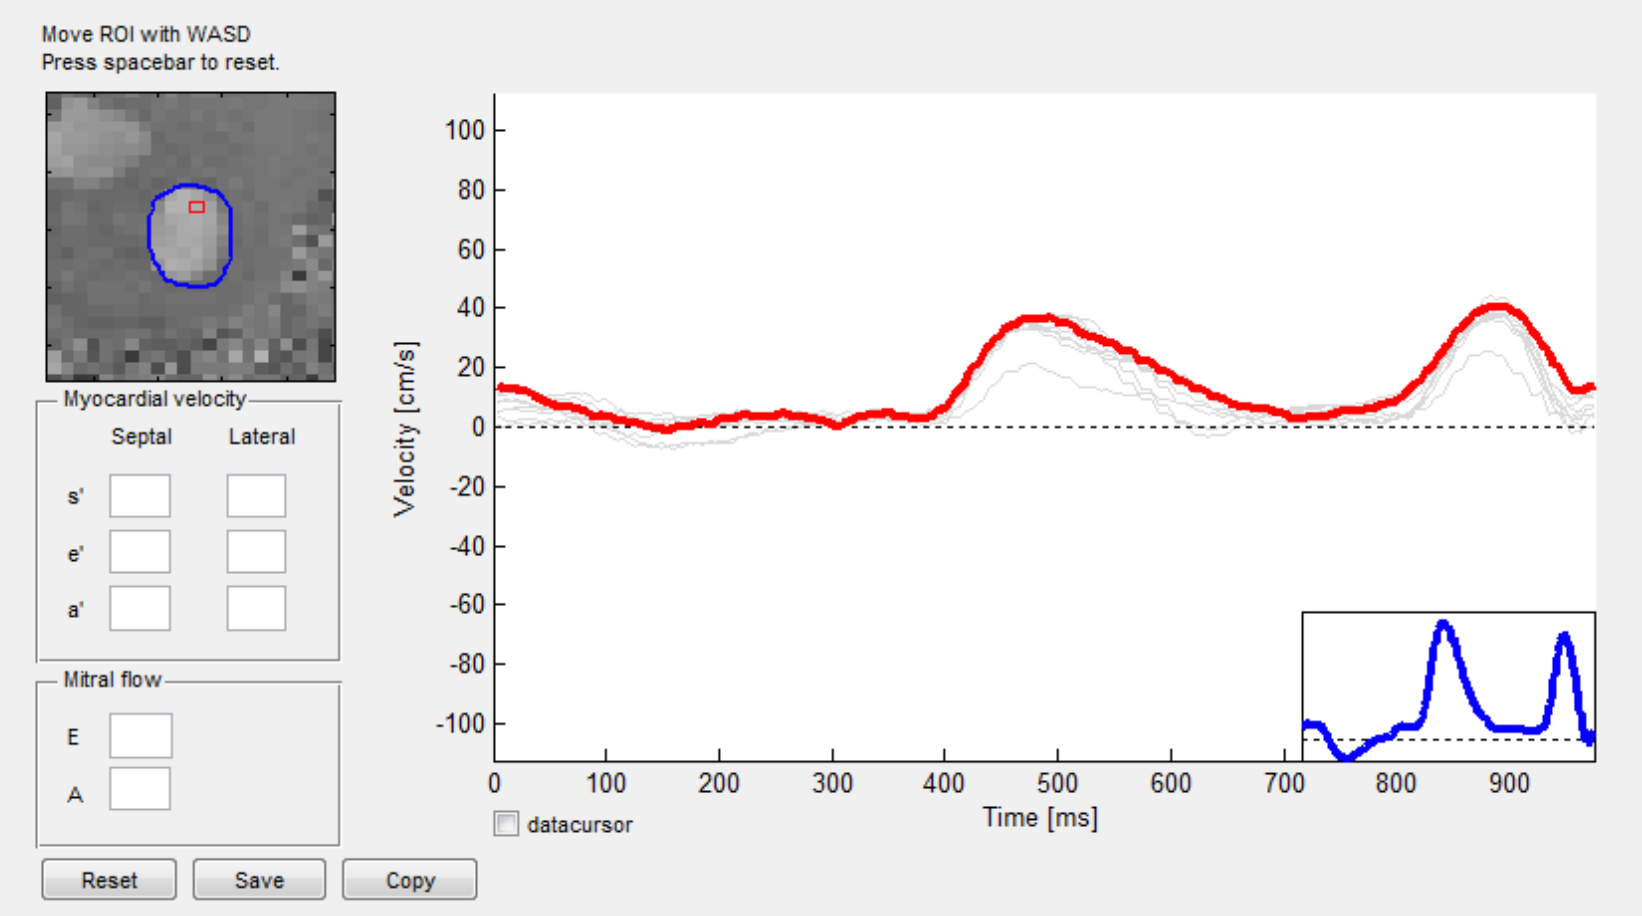
\includegraphics[width=\textwidth]{Figure_3_plugin.png}
    \caption{The measurement graphical user interface (GUI) was implemented as a plugin to the freely available image analysis software, Segment~\cite{Heiberg2010}. The image in the top left corner shows a cine loop of the phase image. The blue ROI indicates the manual identification of the mitral valve orifice, and the red square indicates the currently selected measurement voxel. The velocity in the selected measurement voxel is displayed as a red time-velocity curve in the main window. The average velocity within the blue ROI is displayed as a blue time-velocity curve in the inset window in the bottom right corner. The time-velocity curves in the adjacent (8-connected) voxels are displayed as light gray curves in the background.}
    \label{fig:segment_gui}
\end{figure}

The peak transmitral blood flow velocity was measured in the early filling (E) and late filling (A) phases, as well as the tissue velocity during systole (s'), during early filling (e') and during late filling (a'). The tissue velocities were measured in the lateral wall of the left ventricle and in the septum. Corresponding echocardiographic pulsed-wave Doppler and pulsed-wave tissue Doppler velocity measurements were measured using ViewPoint (GE Healthcare, Chicago, IL).

\subsect{Study IV}
A prototype 3D radial bSSFP pulse sequence was modified to allow for sampling with the 3D-SWIG profile ordering. For further details on the implementation, see Study II. Phantom acquisitions were performed using the conventional double golden-angle profile ordering and one acquisition using the 3D-SWIG profile ordering, using 12, 48 and 192 sectors. For the patients, one acquisition using the conventional double golden-angle profile ordering and one acquisition using the 3D-SWIG profile ordering, using 48 sectors, were acquired in all three subjects. Relevant sequence parameters were TE = 1.7 ms, TR = 3.4 ms, flip angle = $50^\circ$, voxel size 1.2 mm isotropic, for both acquisitions.
\chap{Results}
In this chapter, the most important findings from the four studies will be highlighted. For the full results, see the individual studies.

\sect{Study I}
Study I was a proof-of-concept study to determine if a golden-angle based imaging approach could improve imaging of the pulmonary vasculature, in the context of imaging diagnosis of pulmonary embolism. Diagnosis using MRI had previously been suggested~\cite{Stein2010, Kalb2012, Revel2013}, and in this study, the novel method was compared to a Cartesian free-breathing protocol with multiple repetitions~\cite{Nyren2017}. A number of encoding ordering strategies were tested, i.e. linear ordering, centric ordering, and golden-angle ordering. It was shown that the linear ordering caused the highest degree of image artifacts. The centric ordering scheme somewhat reduced the artifacts, but there was still a severe artifact obscuring the anatomy. Using the golden-angle profile ordering, the artifacts disappeared almost entirely. See figure~\ref{fig:study1_2}.
\begin{figure}[htbp]
    \centering
    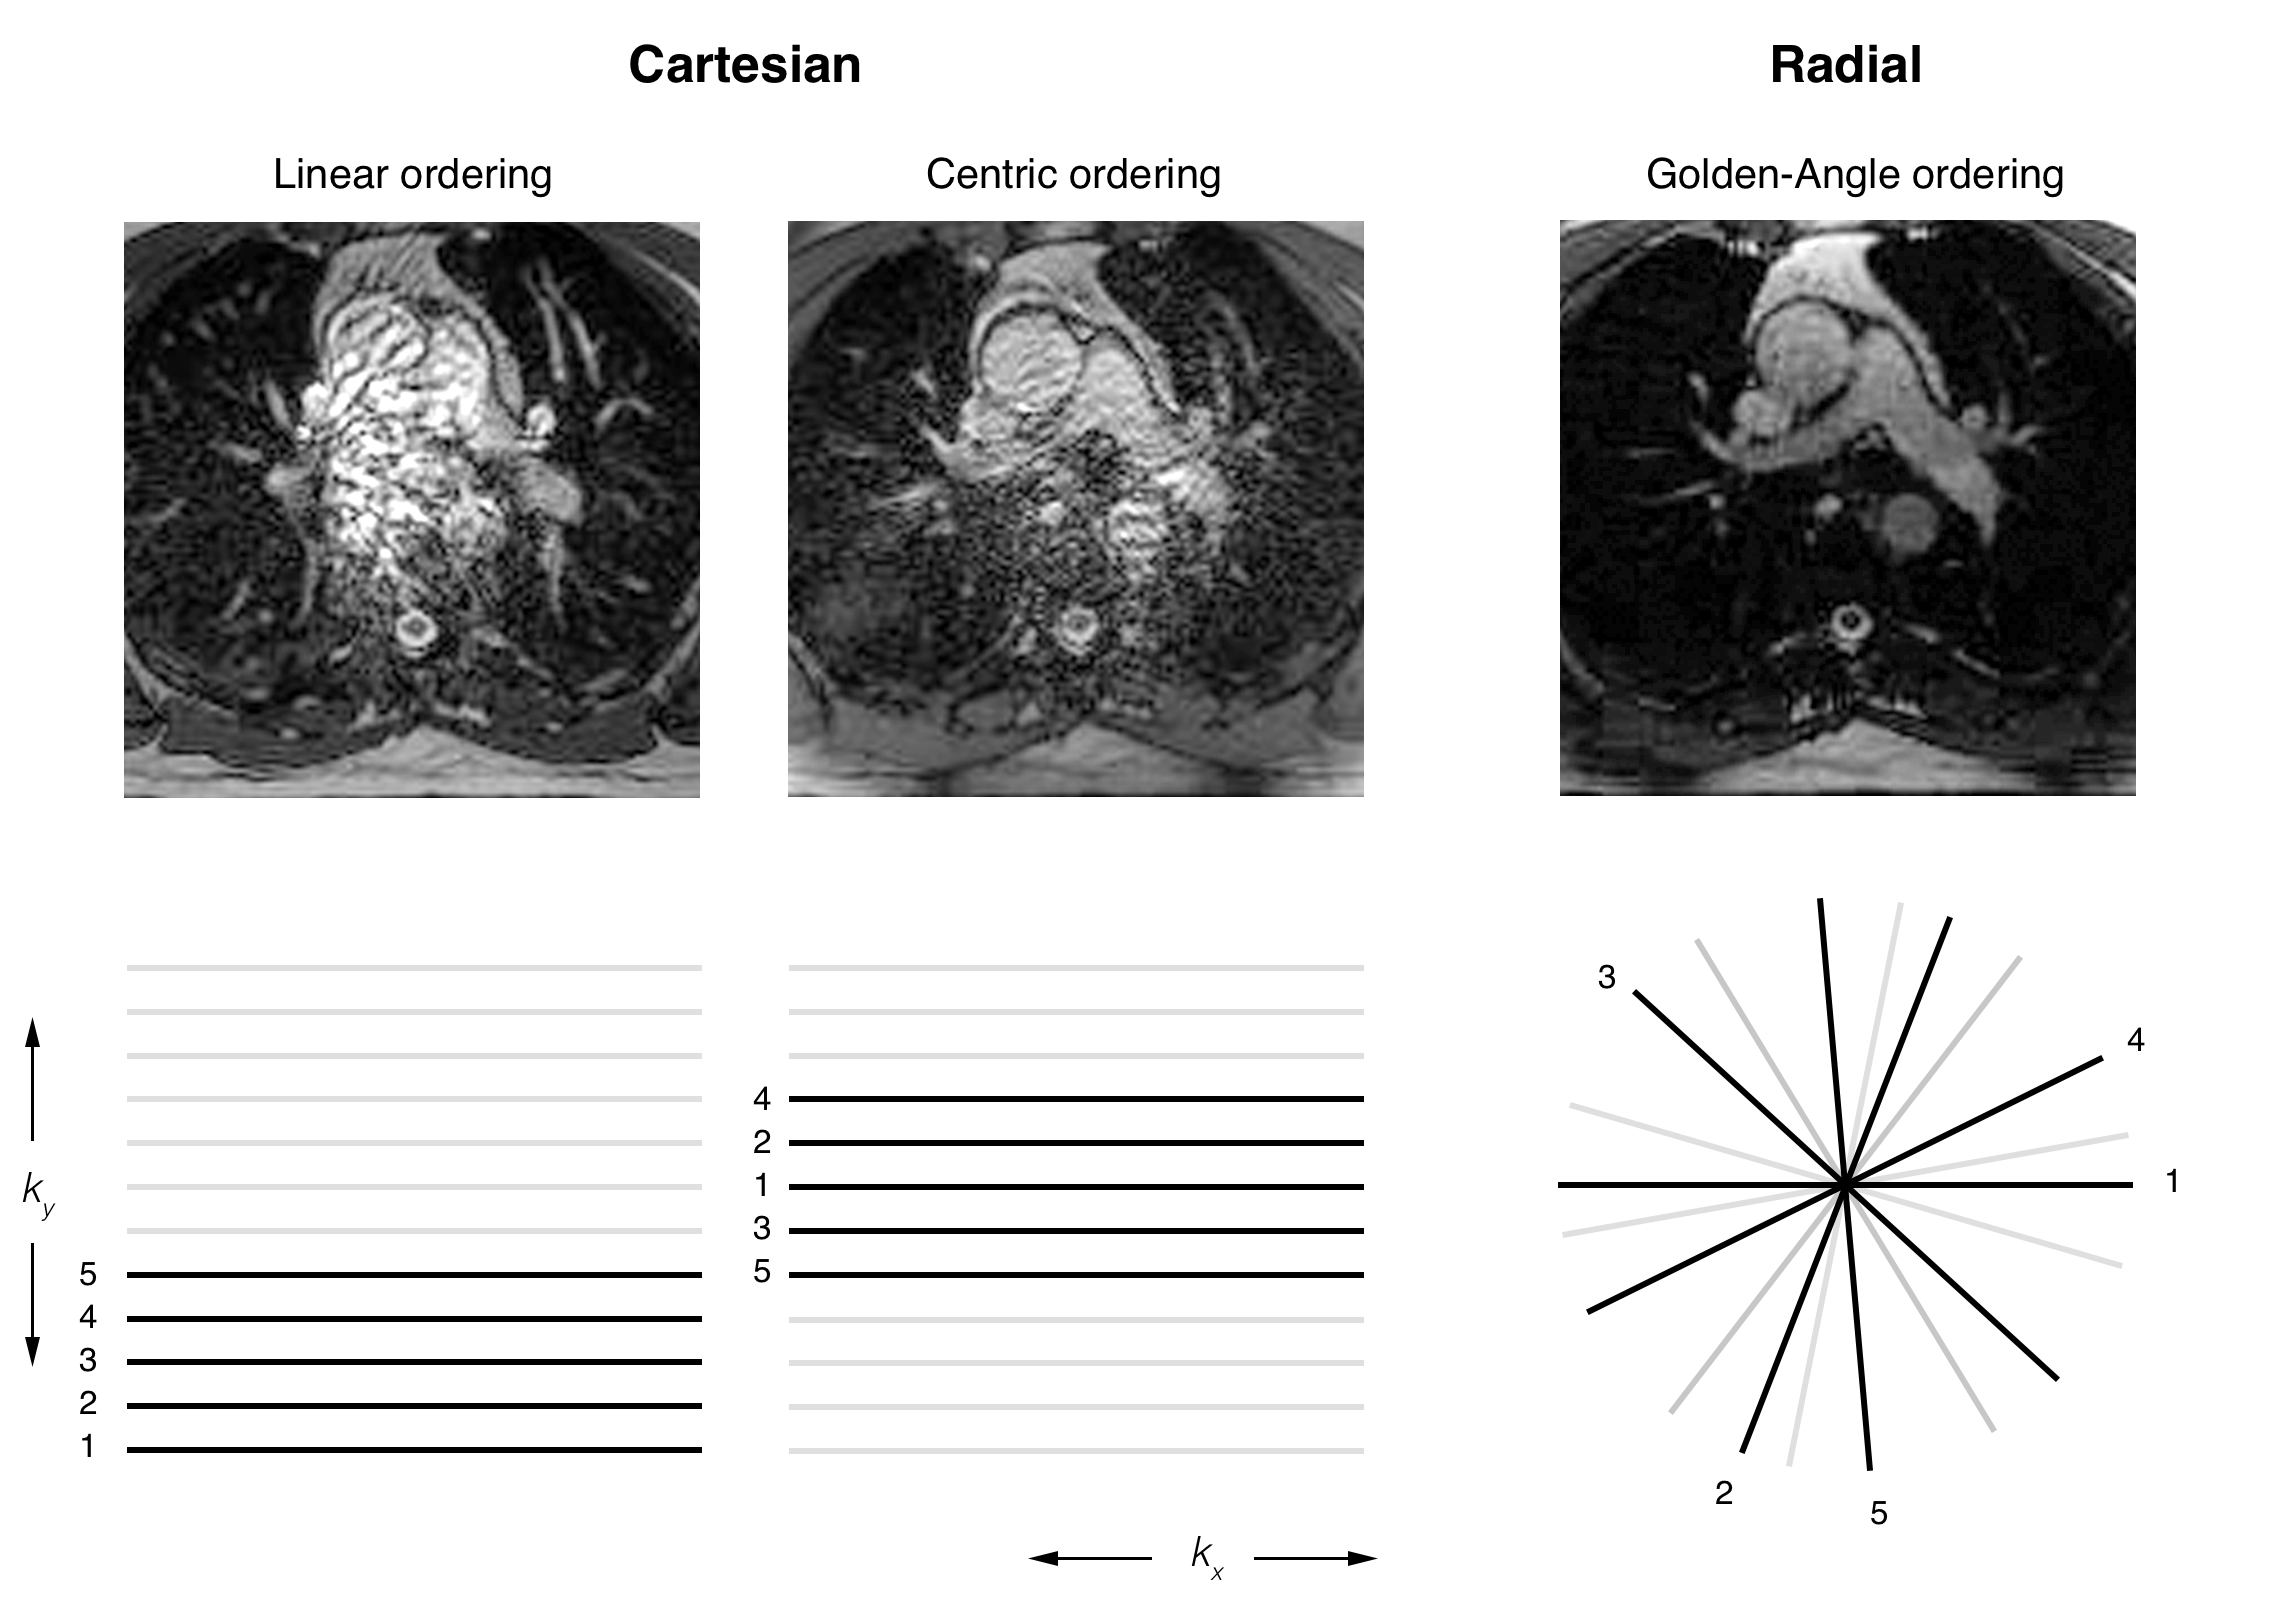
\includegraphics[width=\textwidth]{kspace_ordering}
    \caption{Different k-space orderings and corresponding image quality. Conventional linear ordering shows the highest amount of image artifacts (left), whereas the artifacts are slightly reduced with a centric ordering (middle). Using a golden-angle ordering, there are very little image artifacts present (right). Reproduced with permission from~\cite{Fyrdahl2018}. Copyright \copyright~2018 International Society for Magnetic Resonance in Medicine. Published by John Wiley \& Sons Inc.}
    \label{fig:study1_2}
\end{figure}
The golden-angle approach was evaluated using a sliding-window approach in two patients. A large thrombus was visible in the left pulmonary artery in both subjects. However, there is a clear difference in image quality between the Cartesian and golden-angle acquisitions. To quantify the difference in visibility, the blood-to-blood-clot-contrast was calculated and found to be 23\% higher for the golden-angle acquisition in both cases.
\begin{figure}[htbp]
    \centering
    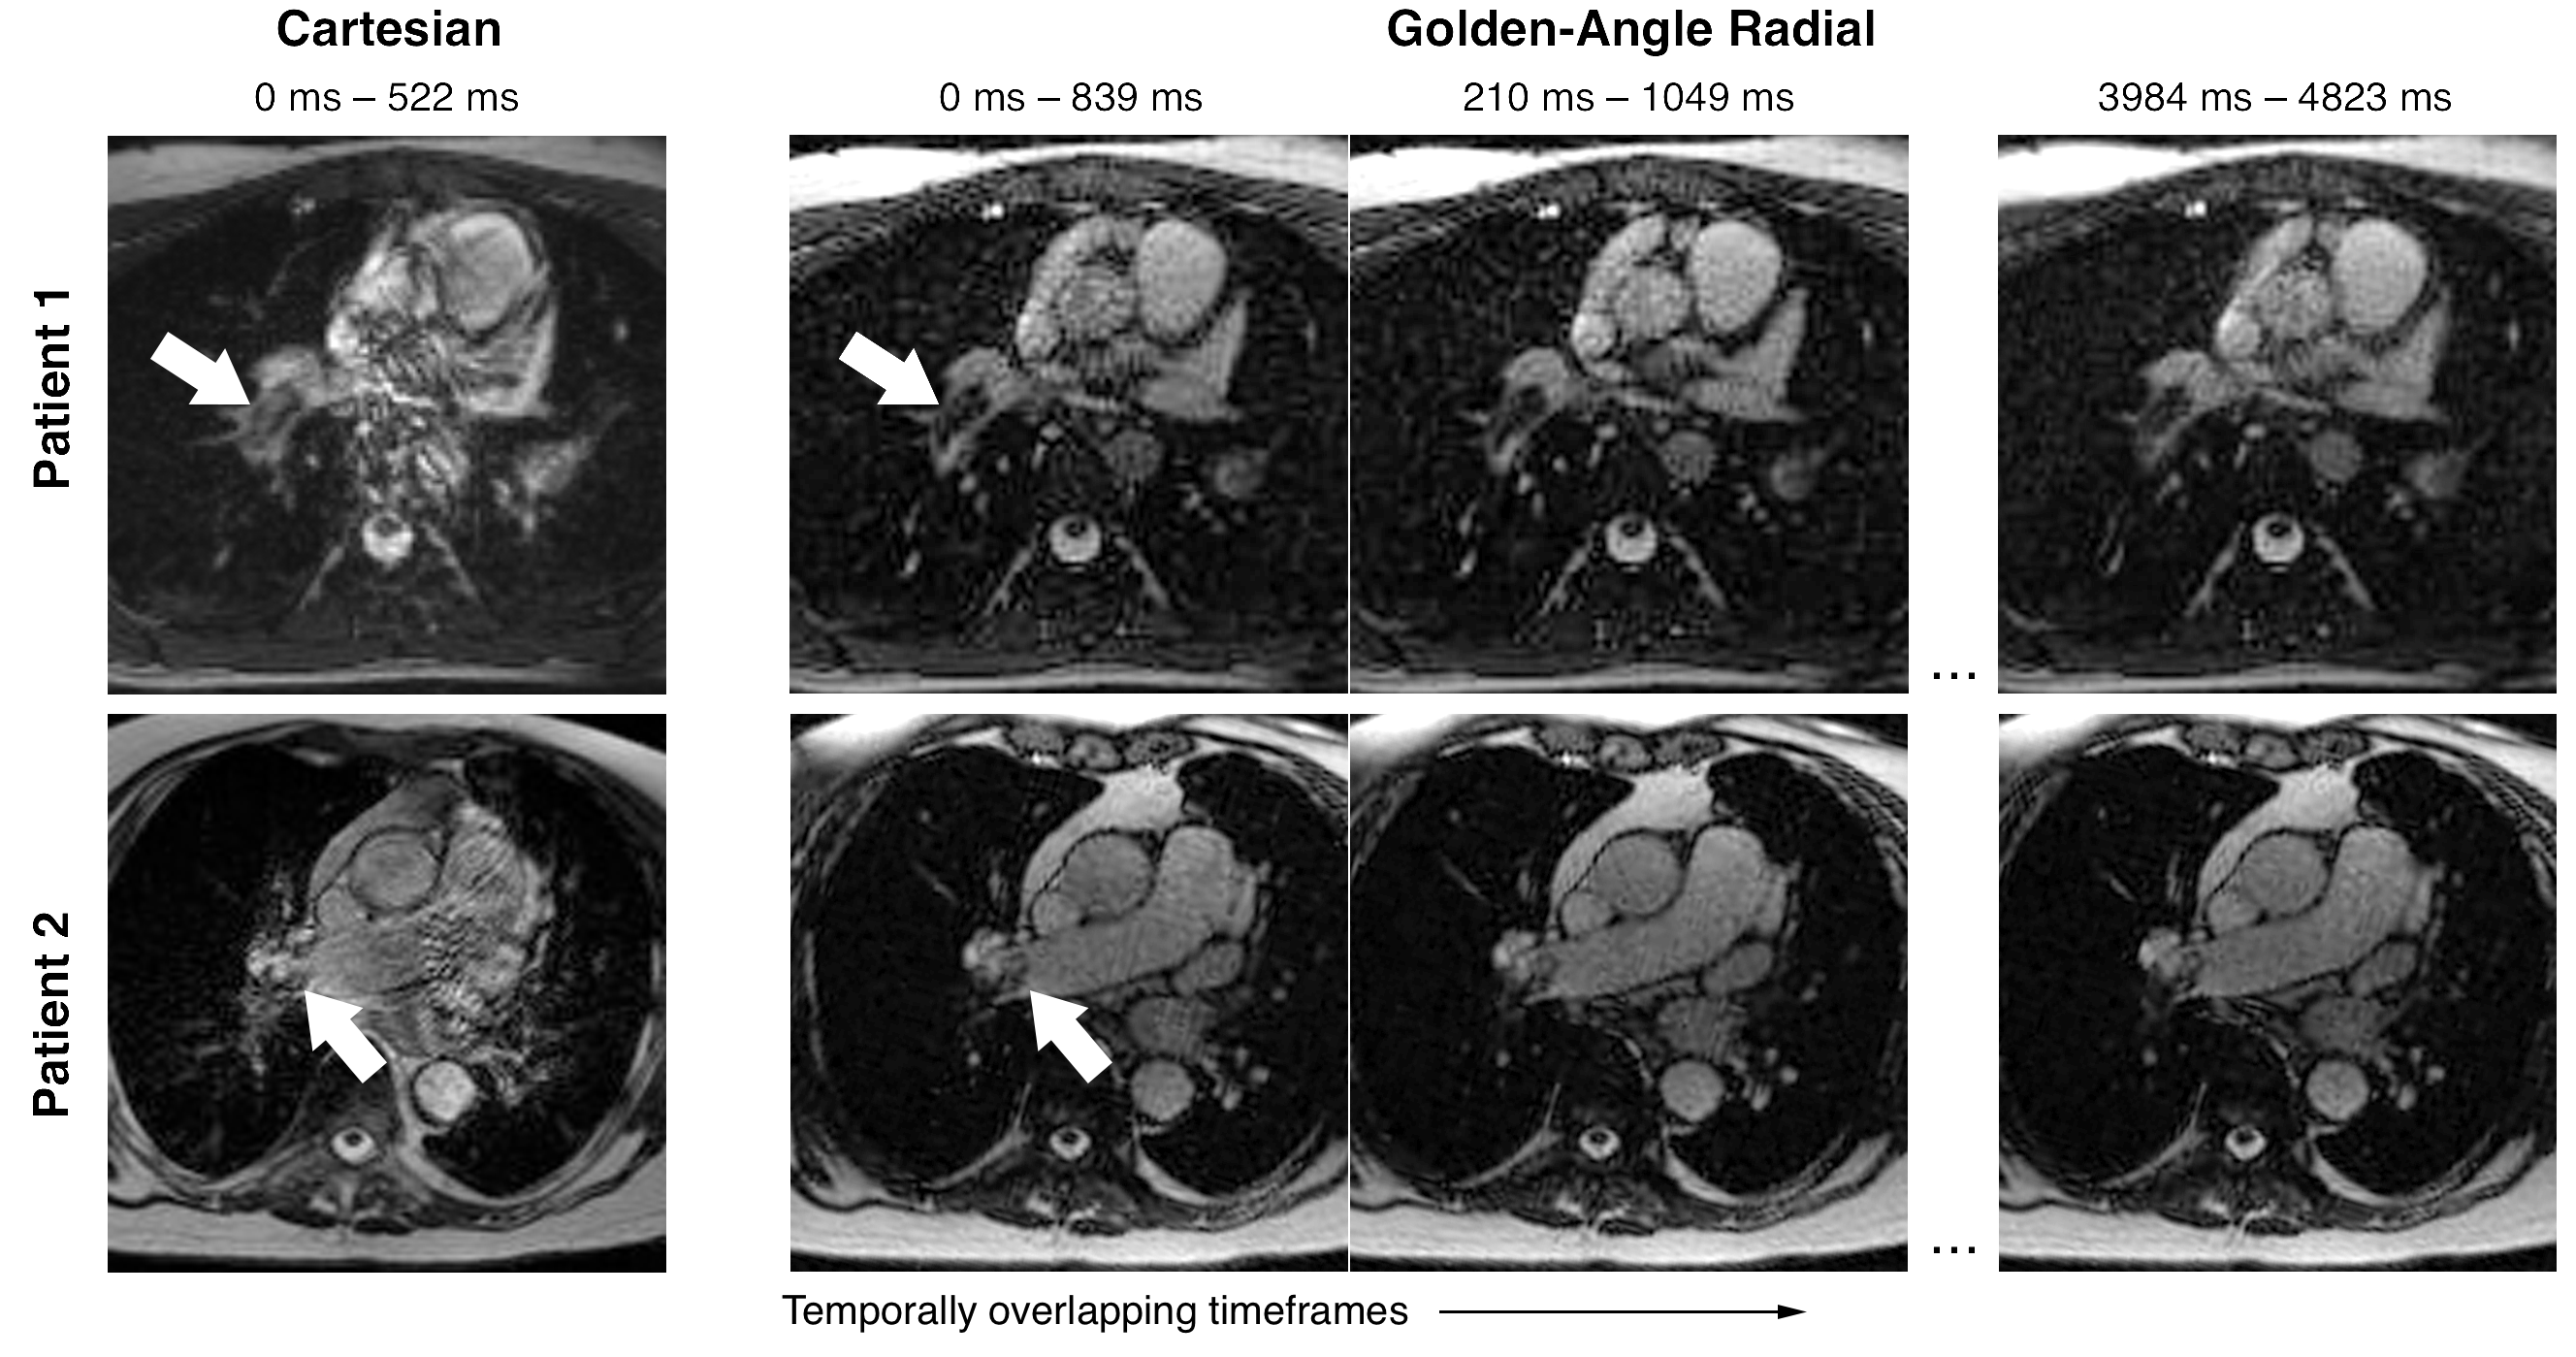
\includegraphics[width=\textwidth]{patients}
    \caption{Representative examples in two different patients with confirmed pulmonary embolism. Cartesian images show a moderate amount of artifacts (left), whereas the golden-angle radial acquisition has less image artifacts (right). The white arrows indicate a thrombus. Reproduced with permission from~\cite{Fyrdahl2018}. Copyright \copyright~2018 International Society for Magnetic Resonance in Medicine. Published by John Wiley \& Sons Inc.}
    \label{fig:study1_3}
\end{figure}
Two experienced observers were asked to score the image quality for the Cartesian and the golden-angle acquisition using three different temporal footprints. The results of the scoring are presented in Table~\ref{table:study1scores}.
\begin{table}[htbp]
\caption{Summary of observer scores for both Cartesian and golden-angle radial, with 144, 610 and 1345 spokes.}
\begin{center}
\begin{threeparttable}
\begin{tabular}{l c c c c}
     \mydarkrowcolor~ & Cartesian & \multicolumn{3}{c}{Golden Angle} \\
     \mydarkrowcolor~ & ~ & 144 spokes & 610 spokes & 1345 spokes \\
     Diagnostic quality & $2.2 \pm 0.6$ & $2.3 \pm 0.7$ & $2.8 \pm 0.8$ & $3.5 \pm 0.9$ \\
     \myrowcolor Vessel sharpness & $2.1 \pm 0.5$ & $2.2 \pm 0.8$ & $2.6 \pm 0.9$ & $3.4 \pm 0.9$ \\
     Artifacts & $3.0 \pm 1.0$ & $3.0 \pm 0.9$ & $3.4 \pm 0.8$ & $3.9 \pm 0.7$ \\
     \bottomrule
\end{tabular}
\begin{tablenotes}
\emph{Note:} Continuous values are presented as mean $\pm$ SD. Higher scores means better images.
\end{tablenotes}
\end{threeparttable}
\end{center}
\label{table:study1scores}
\end{table}

\sect{Study II}
In study II, a modified 3D-radial double golden angle profile ordering was proposed to reduce eddy current artifacts. The proposed profile orderings showed a uniform behavior, in comparison to a completely random profile ordering, see Figure~\ref{fig:study2_1}, which was also confirmed by numerical calculations of the CCR-continuum.
\begin{figure}[htbp]
    \centering
    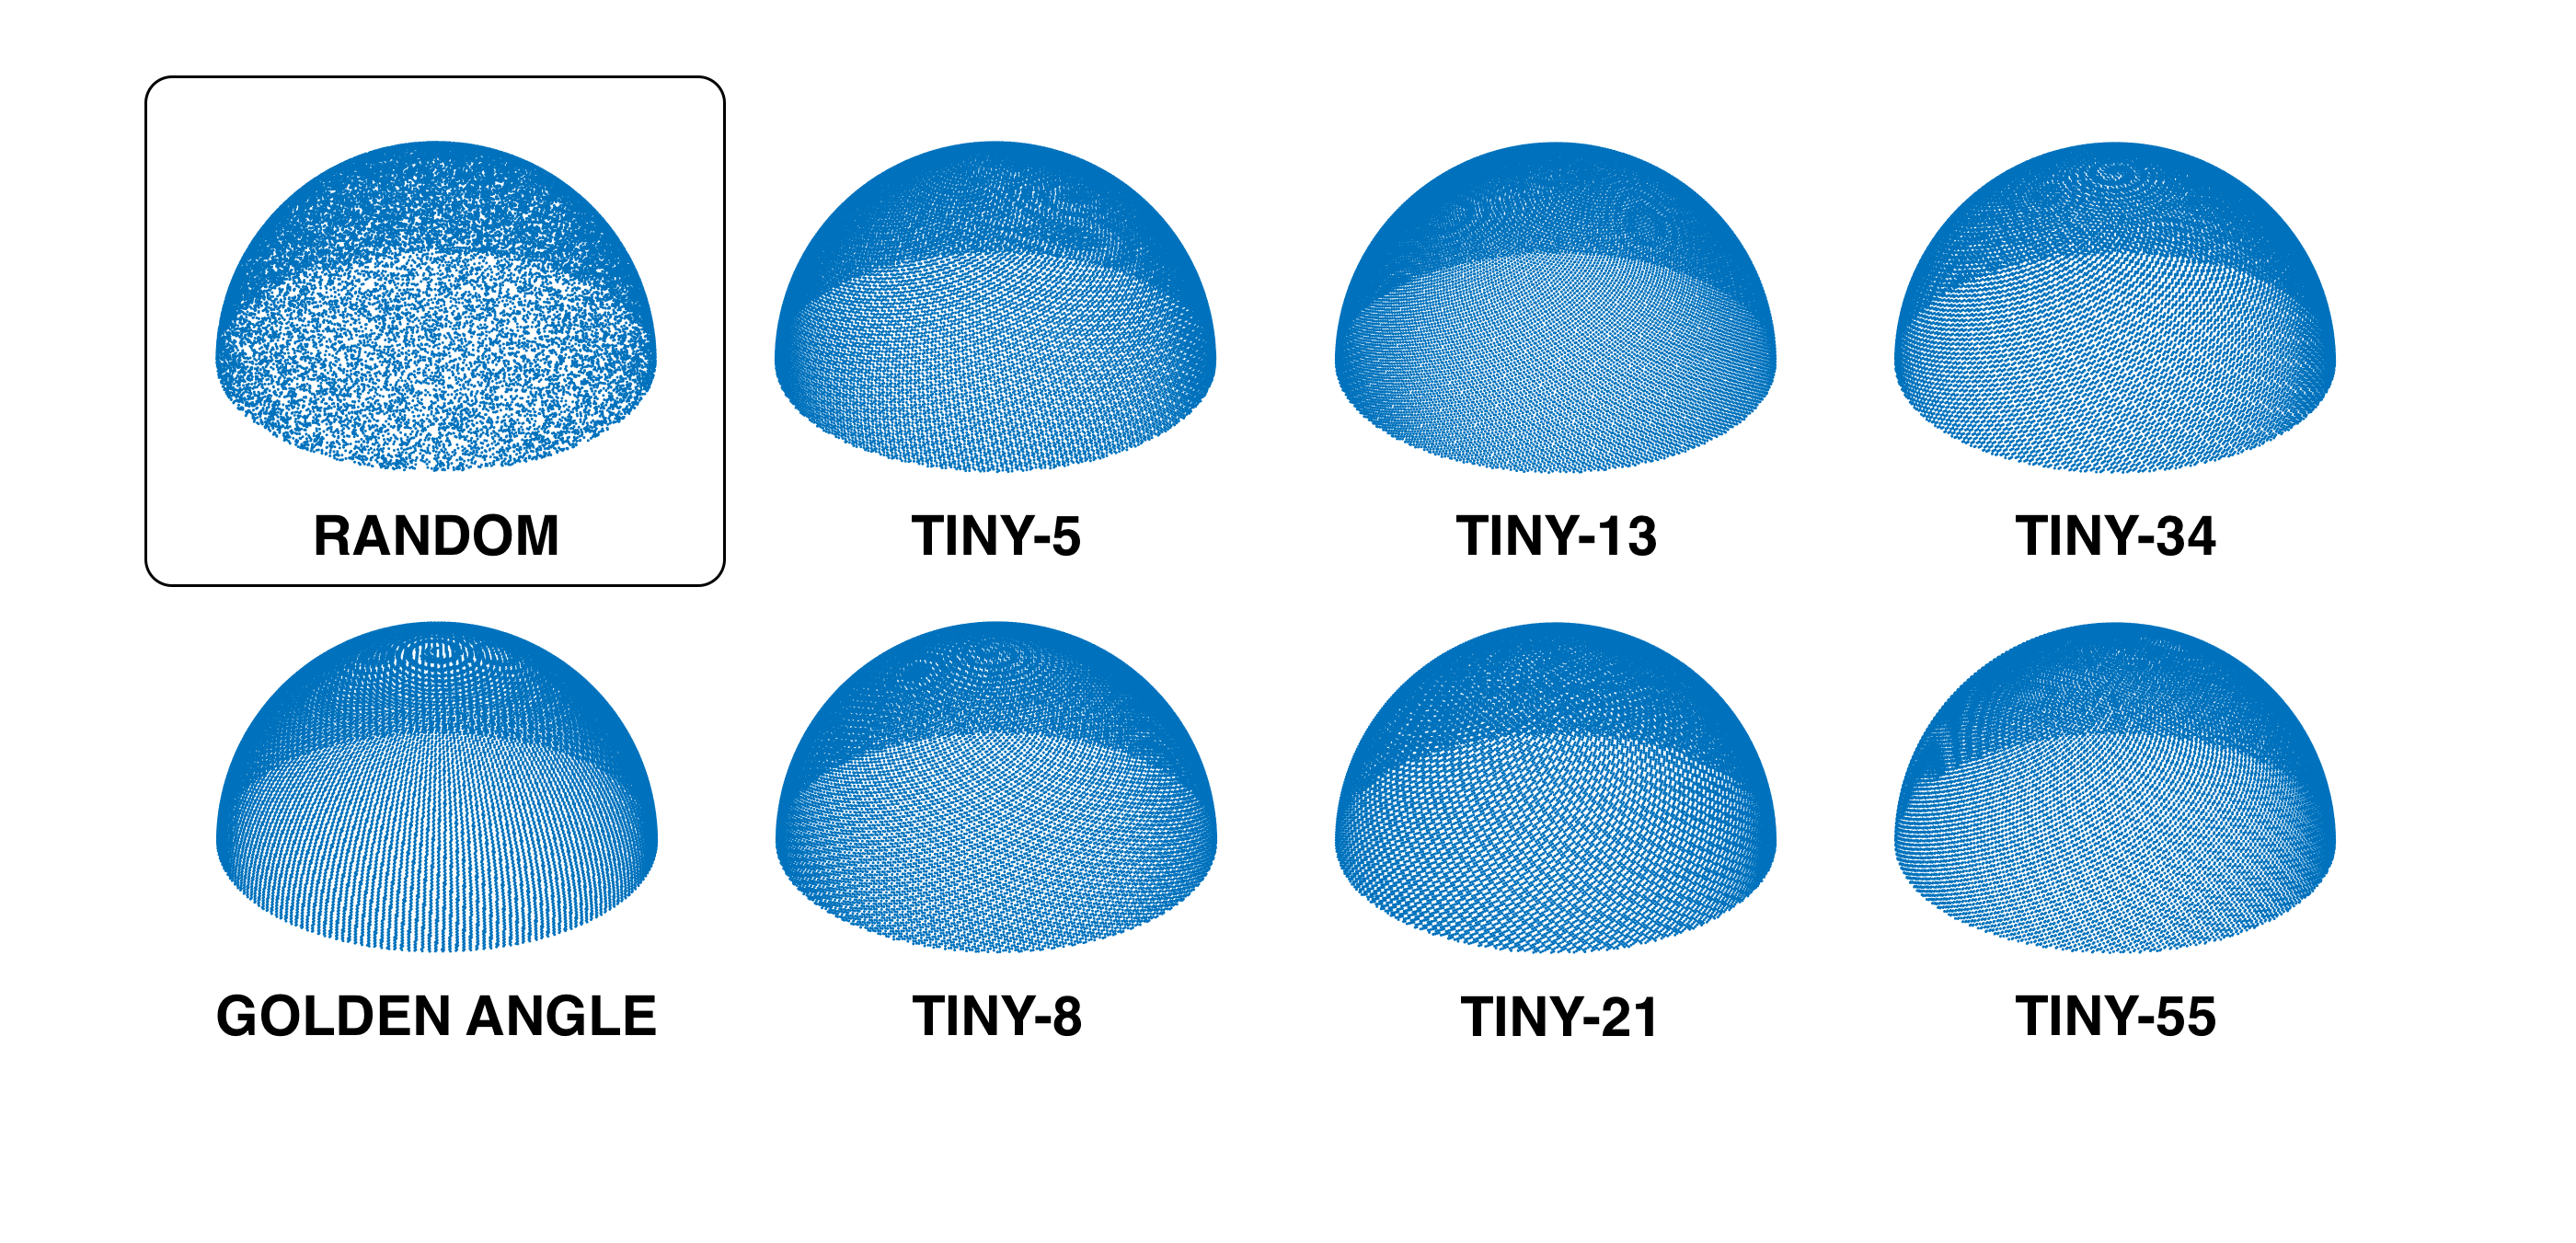
\includegraphics[width=\textwidth]{fig_1_trajectories.png}
    \caption{A completely random profile ordering (black box) compared to the original double golden angle profile ordering as well as Tiny 5, 8, 13, 21, 34 and 55. There is an apparent uniformity to the golden, and tiny profile orderings, which is not present in the random distribution. This finding is corroborated by the CRR measure.}
    \label{fig:study2_1}
\end{figure}
One profile ordering, Tiny-13, was chosen for further testing. It was compared to the original double golden angle profile ordering~\cite{Chan2009}, by performing a simulated physiological binning based on pre-recorded ECG and respiratory signals. Binning was performed into 20 and 25 cardiac phases as well as 2, 4 and 6 respiratory bins. The profile ordering was calculated for all time frames for both profile orderings. Tiny-13 showed a higher degree of k-space uniformity in all cases except for 25 cardiac phases and 6 respiratory bins, where differences did not reach statistical significance.
\begin{figure}[htbp]
    \centering
    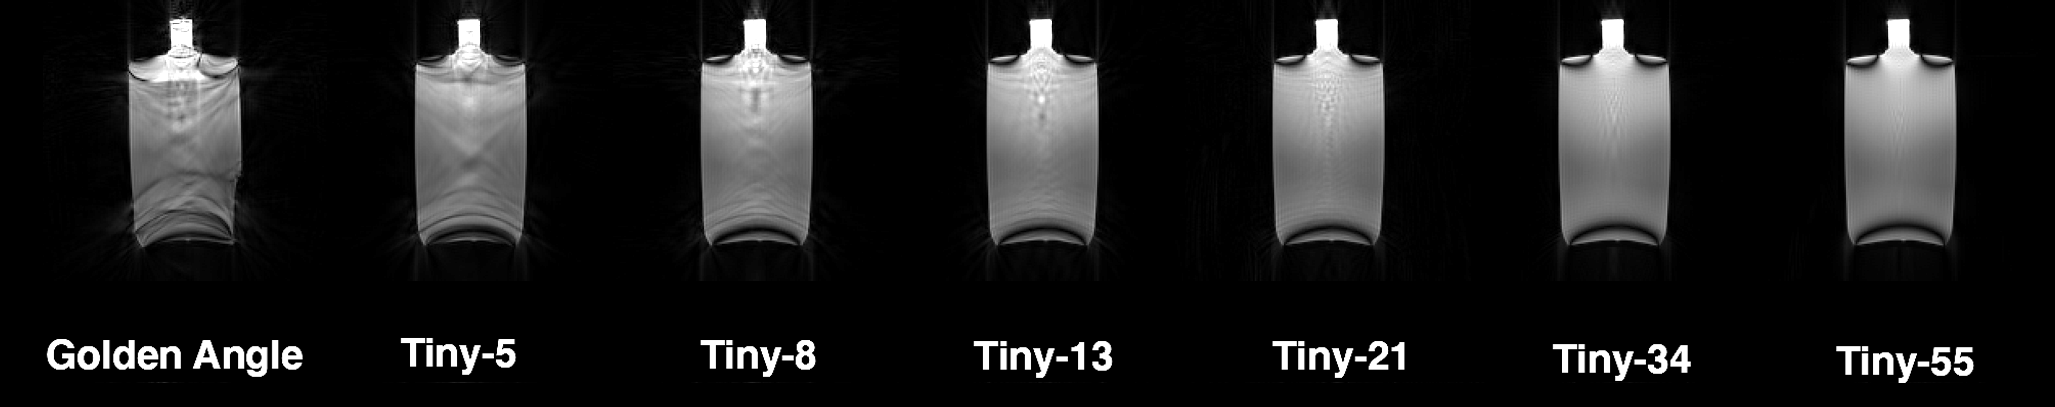
\includegraphics[width=\textwidth]{phantom_modified.png}
    \caption{Phantom acquisitions of the original double golden angle profile ordering and Tiny 5, 8, 13, 21, 34 and 55 (from left to right). There is a gradual decrease in image artifacts with a decreasing angle between successive readouts.}
    \label{fig:study2_2}
\end{figure}
\begin{figure}[htbp]
    \centering
    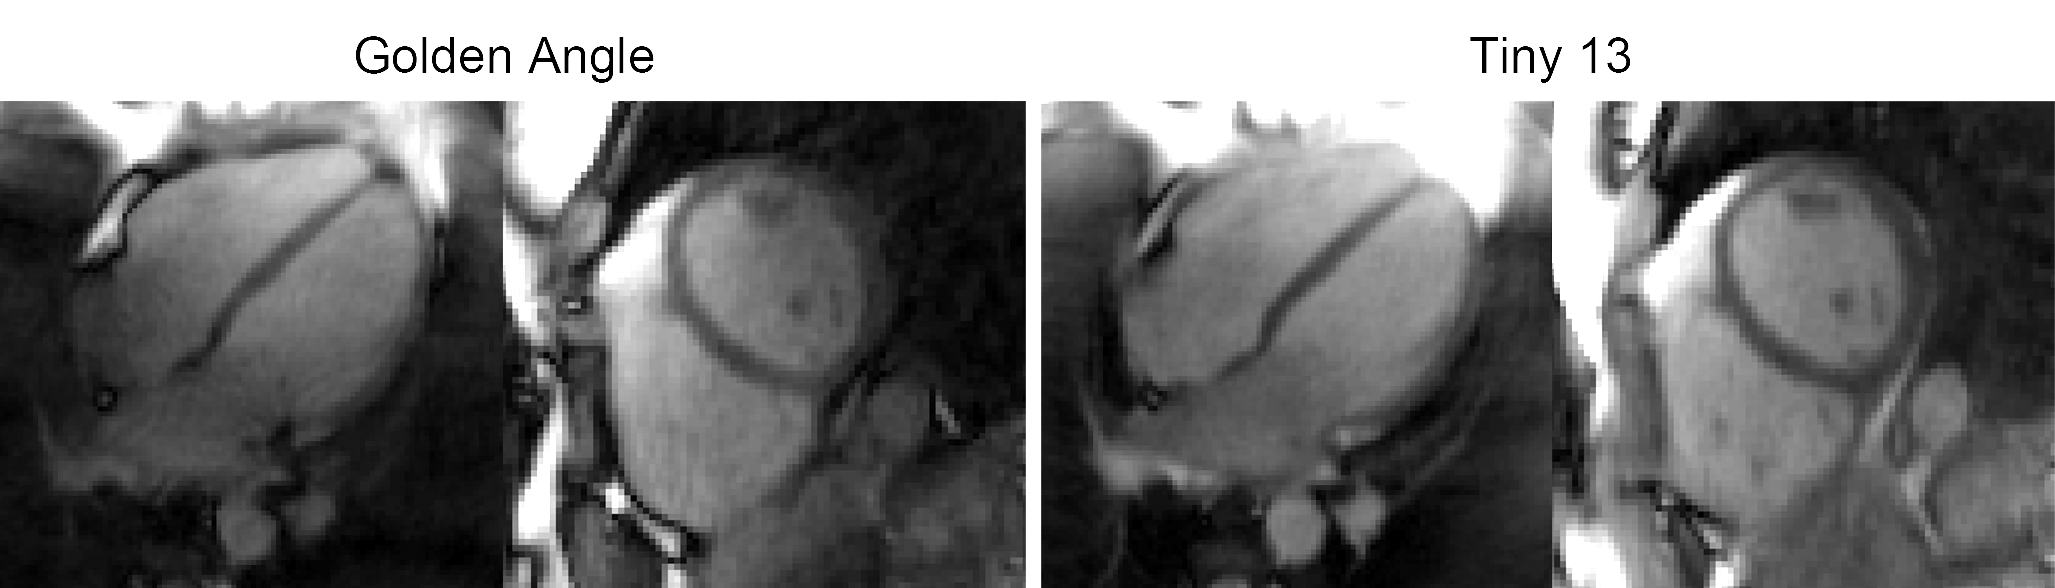
\includegraphics[width=\textwidth]{in_vivo_modified_lighter.png}
    \caption{\emph{In vivo} measurements in a healthy volunteer with the original double golden angle profile ordering (left) and the proposed Tiny-13 profile ordering (right) show a maintained ability to perform physiological binning, and an improvement in the image homogeneity with the reduced angular step.}
    \label{fig:study2_3}
\end{figure}
\sect{Study III}
In Study III, a modified golden-angle phase contrast pulse sequence was proposed and evaluated for measurements of transmitral blood-flow and tissue velocities in patients. The PSF-analysis showed a higher sampling uniformity, and subsequently a lower peak PSF as a function of radius for the SWIG method compared to conventional golden-angle, see Figure~\ref{fig:study3_1}.

\begin{figure}[htbp]
    \centering
    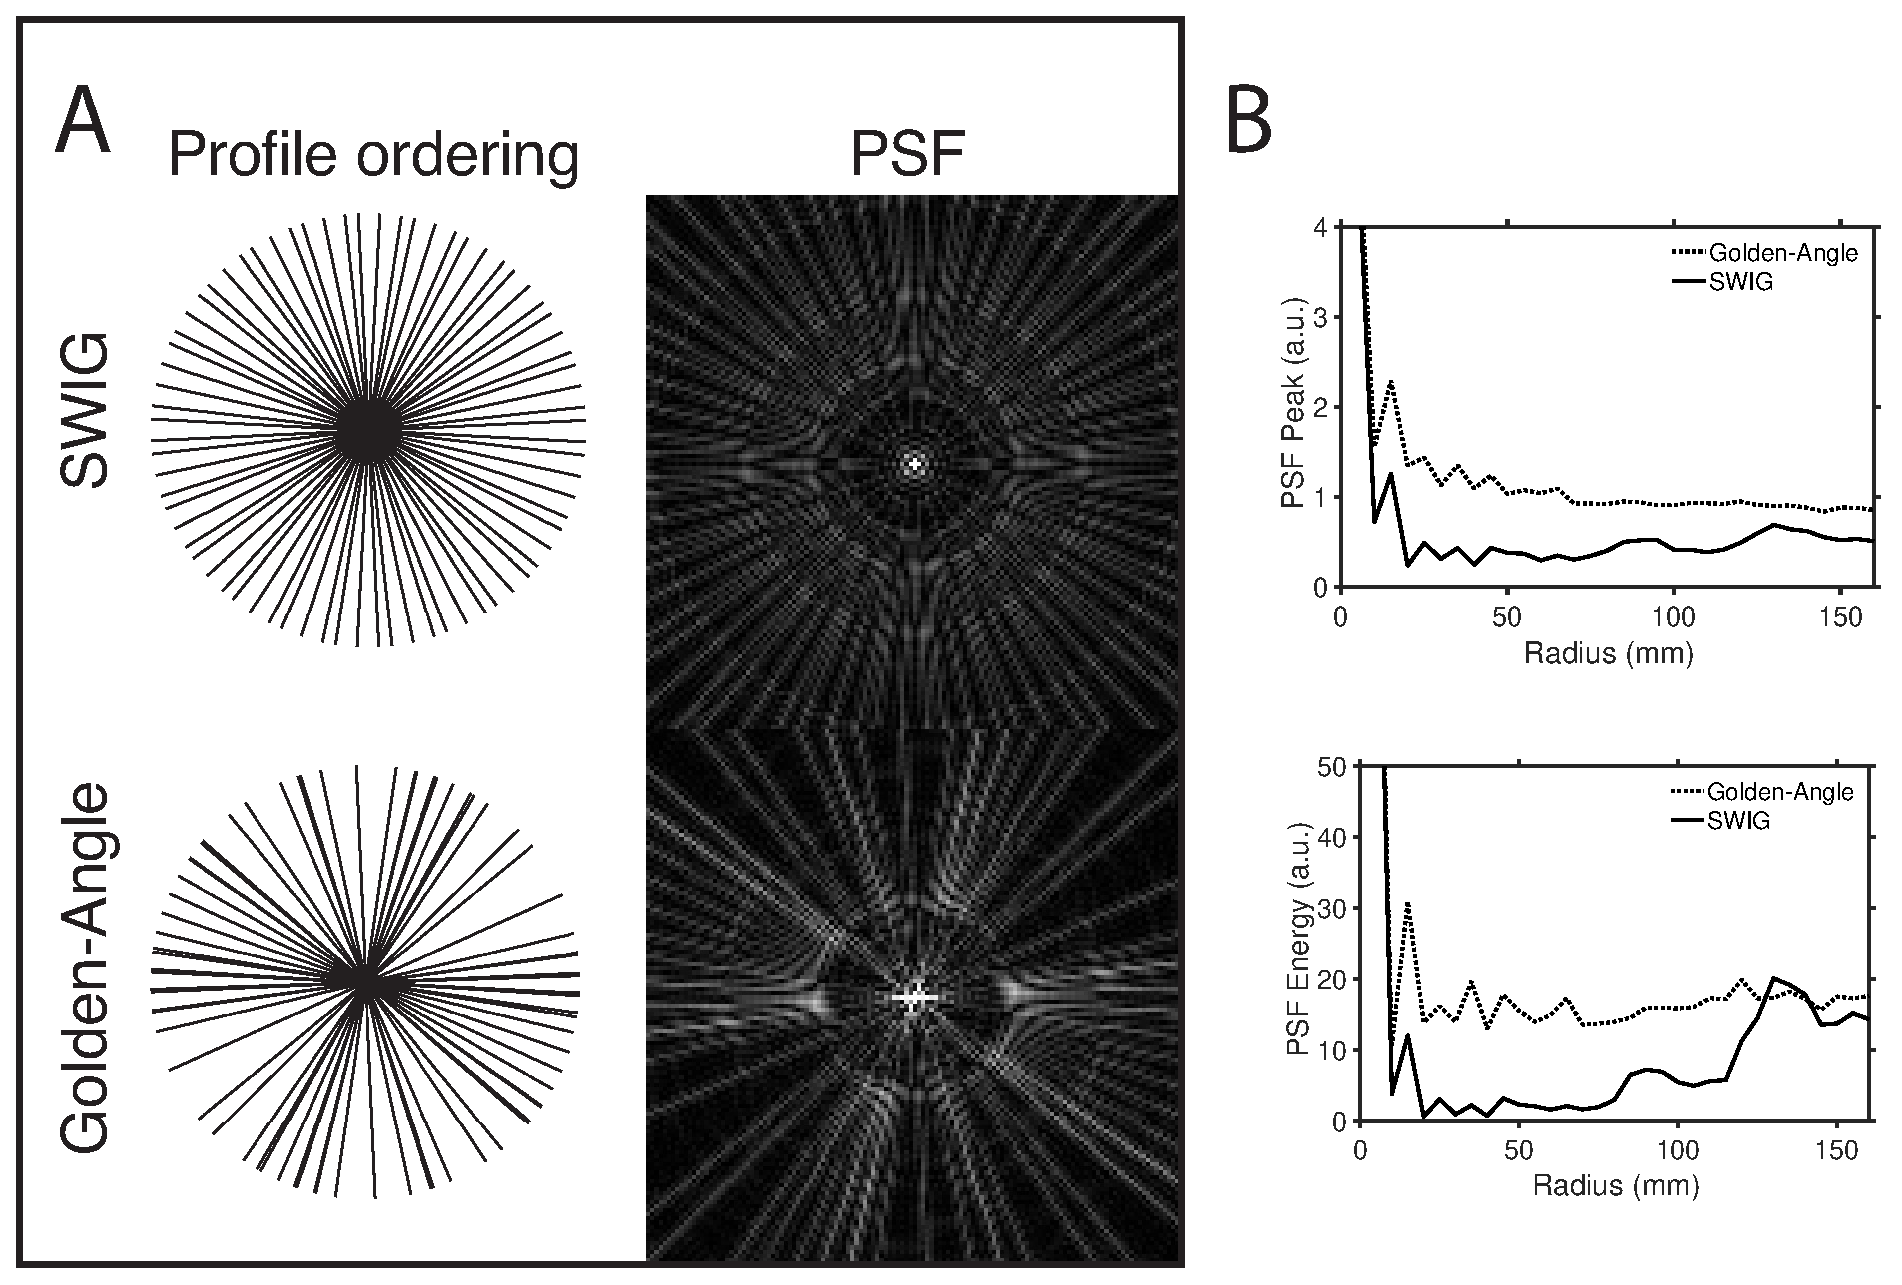
\includegraphics[width=\textwidth]{Figure_2_PSF}
    \caption{Examples of the k-space sampling distribution and the corresponding PSF for both SWIG and the conventional golden-angle profile ordering (A). The peak PSF and PSF energy as a function of radius (B). Reproduced from~\cite{Fyrdahl2020}. (Licensed under CC-BY-4.0)}
    \label{fig:study3_1}
\end{figure}

The pilot study showed that depending on the temporal footprint selected, CMR could either underestimate or overestimate the velocities compared to tissue Doppler echocardiography, see Figure~\ref{fig:study3_abstract}. It was clear that a smaller temporal footprint produced a sharper velocity peak, however, at the expense of increased noise, see Figure~\ref{fig:study3_2}. For a summary of the results from the pilot study, see Table~\ref{table:study3footprint}.

\begin{figure}[htbp]
    \centering
    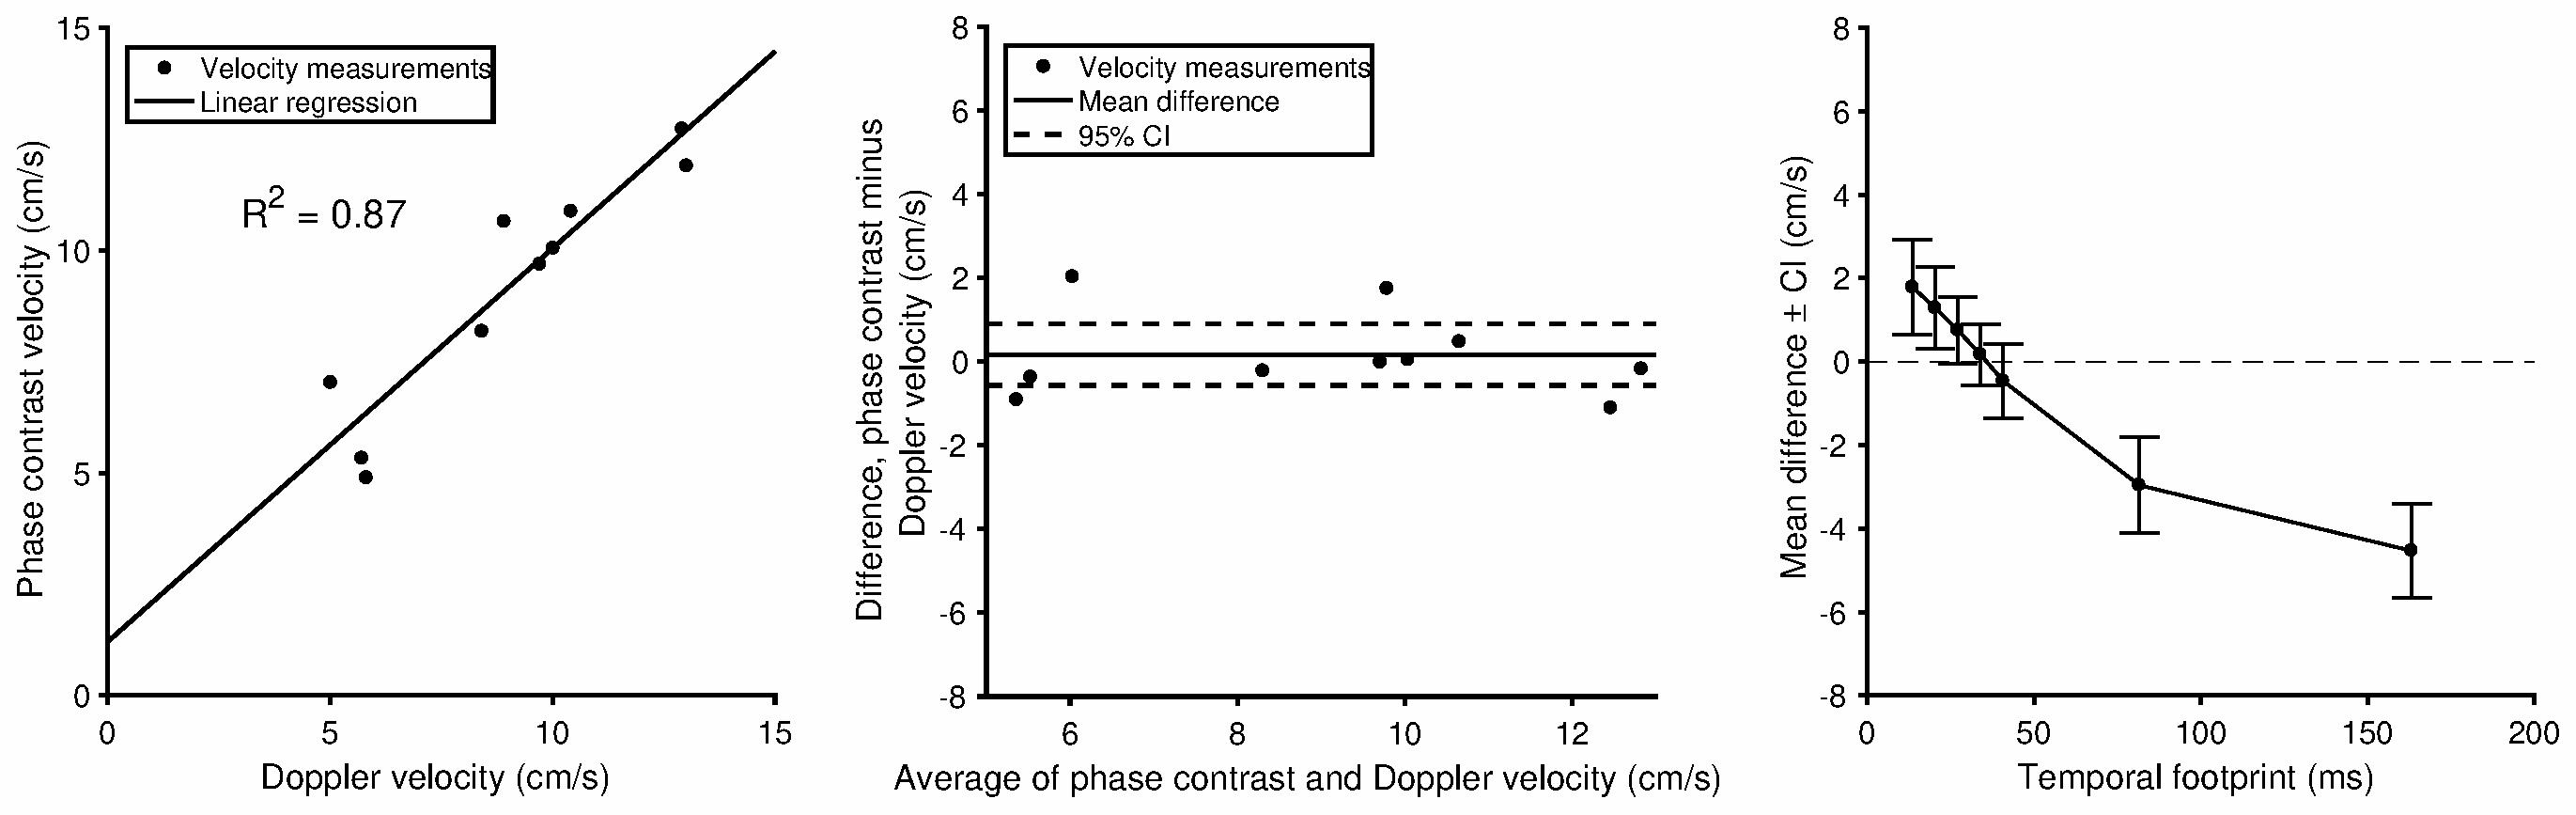
\includegraphics[width=\textwidth]{corr_6}
    \caption{Results from the pilot study. The correlation is shown for a temporal footprint for CMR of 34 ms (left) with corresponding Bland-Altman plot (middle). A temporal footprint between 27.2 ms and 40.8 ms did not differ when compared between CMR and tissue Doppler. Using larger footprints for CMR resulted in an apparent underestimation, whereas using a smaller temporal footprint resulted in an apparent overestimation of the tissues velocities compared to tissue Doppler (right). Reproduced from~\cite{Fyrdahl2018:SCMR}.}
    \label{fig:study3_abstract}
\end{figure}


\begin{figure}[htbp]
    \centering
    \includegraphics[width=\textwidth]{Figure_3_Multiple_resolutions}
    \caption{Representative phase contrast images in systole, early filling and late filling (A). Time velocity curves measured in a single voxel in the lateral wall. Different colors represents different temporal footprints. The black box indicates the early filling velocity peak (B). A magnified view of the early filling peak (C). Reproduced from~\cite{Fyrdahl2020}. (Licensed under CC-BY-4.0)}
    \label{fig:study3_2}
\end{figure}

\begin{table}[htbp]
\caption{Comparison between CMR-derived and Doppler-derived myocardial velocities in early filling (e') with a variable temporal footprint and a fixed temporal increment.}
\begin{center}
\begin{threeparttable}
\begin{tabular}{c c c c c c c}
     \mydarkrowcolor \multicolumn{3}{c}{\textbf{Temporal footprint}} & \textbf{Correlation} & \textbf{Mean difference} & \textbf{95\% LoA} & \textbf{P} \\
     \mydarkrowcolor \quad & (TR) & (ms) & (R$^2$) & (cm/s) & (cm/s) & ~\\
     \quad & 4 & 27.2 & 0.46 & 1.0 & 4.3 & 0.03 \\
     \myrowcolor \quad & 6 & 40.8 & 0.63 & 0.9 & 3.4 & 0.13 \\
     \quad & 8 & 54.5 & 0.72 & 0.4 & 3.0 & 0.41 \\
     \myrowcolor \quad & 10 & 68.0 & 0.69 & -0.2 & 3.3 & 0.71 \\
     \quad & 12 & 81.6 & 0.65 & -0.9 & 3.5 & 0.14 \\
     \bottomrule
\end{tabular}
\begin{tablenotes}
\emph{Note:} P-values denote outcome of Mann-Whitney U-test with the null hypothesis that the CMR and Doppler velocities did not differ. LoA – Limits of Agreement.\\
\end{tablenotes}
\end{threeparttable}
\end{center}
\label{table:study3footprint}
\end{table}

The patient study showed a high degree of correlation for measurement of tissue velocities but a systematic underestimation of transmitral blood flow velocities, see Figure~\ref{fig:study3_3}. For a summary of all results from the patient study, see Table~\ref{table:study3summary}.

\begin{figure}[htbp]
    \centering
    \includegraphics[width=\textwidth]{Figure_5_Myo+Mitral}
    \caption{Scatter plot (A) and the corresponding Bland-Altman plot (B) for myocardial tissue velocities (s’, e’, a’) measured separately in the septal and lateral wall with both tissue Doppler echocardiography and phase contrast CMR. Scatter plot (C) and the corresponding Bland-Altman plot (D) for peak transmitral velocities (E, A) measured with both Doppler echocardiography and phase contrast CMR. Reproduced from~\cite{Fyrdahl2020}. (Licensed under CC-BY-4.0)}
    \label{fig:study3_3}
\end{figure}

\begin{table}[htbp]
\caption{Comparison between CMR-derived and Doppler-derived myocardial velocities in early filling (e') with a variable temporal footprint and a fixed temporal increment.}
\begin{center}
\begin{threeparttable}
\begin{tabular}{c c c c c c c}
     \mydarkrowcolor \multicolumn{7}{l}{\textbf{Myocardial velocity}} \\
     \mydarkrowcolor ~ & \textbf{Doppler} & \textbf{CMR} & \textbf{P} & \textbf{Correlation} & \textbf{Mean diff.} & \textbf{95\% LoA} \\
     \mydarkrowcolor ~ & (cm/s) & (cm/s) & ~ & (R$^2$) & (cm/s) & (cm/s) \\ 
     All & $8.2 \pm 3.0$ & $9.0 \pm 3.0$ & $<0.005$ & $0.63$ & $0.9$ & $\pm 3.7$ \\
     \myrowcolor s' & $7.1 \pm 1.8$ & $8.1 \pm 2.1$ & $<0.005$ & $0.34$ & $1.0$ & $\pm 3.4$ \\
     e' & $8.1 \pm 2.7$ & $9.1 \pm 3.1$ & $<0.005$ & $0.74$ & $0.8$ & $\pm 3.5$ \\
     \myrowcolor a' & $9.4 \pm 3.5$ & $10.2 \pm 3.3$ & $< 0.005$ & $0.54$ & $1.0$ & $\pm 4.2$ \\
     \mydarkrowcolor \multicolumn{7}{l}{\textbf{Transmitral blood flow velocity}} \\
     \mydarkrowcolor ~ & \textbf{Doppler} & \textbf{CMR} & \textbf{P} & \textbf{Correlation} & \textbf{Mean diff.} & \textbf{95\% LoA} \\
     \mydarkrowcolor ~ & (cm/s) & (cm/s) & ~ & (R$^2$) & (cm/s) & (cm/s) \\
    All & $67 \pm 18$ & $56 \pm 16$ & $<0.005$ & $0.45$ & $-11$ & $\pm 28$ \\
    \myrowcolor E & $74 \pm 17$ & $60 \pm 15$ & $<0.005$ & $0.27$ & $-14$ & $\pm 31$ \\
    A & $60 \pm 17$ & $51 \pm 17$ & $<0.005$ & $0.53$ & $-8$ & $\pm 25$ \\
    \mydarkrowcolor \multicolumn{7}{l}{\textbf{Derived parameters}} \\
     \mydarkrowcolor ~ & \textbf{Doppler} & \textbf{CMR} & \textbf{P} & \textbf{Correlation} & \textbf{Mean diff.} & \textbf{95\% LoA} \\
     \mydarkrowcolor ~ & (a.u) & (a.u) & ~ & (R$^2$) & (a.u.) & (a.u.) \\ 
    E/e'& $8.58 \pm 3.28$ & $6.25 \pm 2.28$ & $<0.005$ & $0.34$ & $-2.3$ & $\pm 5.3$ \\
    \myrowcolor E/A & $1.34 \pm 0.50$ & $1.31 \pm 0.55$ & $0.295$ & $0.66$ & $0.03$ & $\pm 0.6$ \\
\end{tabular}
\begin{tablenotes}
\emph{Note:} Continuous values are presented as mean $\pm$ SD. P-values denote outcome of Mann-Whitney U-test with the null hypothesis that the CMR and Doppler velocities did not differ. LoA – Limits of Agreement.\\
\end{tablenotes}
\end{threeparttable}
\end{center}
\label{table:study3summary}
\end{table}

\sect{Study IV}
The result from the PSF-analysis showed that for high undersampling factors, i.e., 12 patches, there was a clear difference in the PSF between the double golden-angle profile ordering and the 3D-SWIG profile ordering. For 48 patches and 192 patches (R=1), the difference was less prominent, albeit with a slight edge to the 3D-SWIG profile ordering, see Figure~\ref{fig:study4_1}. For the three subjects, the k-space uniformity was significantly higher for SWIG-3D compared to the double golden-angle profile ordering, see Figure~\ref{fig:study4_2}.
\begin{figure}[htbp]
    \centering
    \includegraphics[width=\textwidth]{Fig5_PSF}
    \caption{Examples of the PSF for both 3D-SWIG and the conventional double golden-angle profile ordering for 12, 48 and 192 sectors (left). The aliasing a function of radius show a difference for 12 sectors, but a decreasing difference as the number of sectors is increased.}
    \label{fig:study4_1}
\end{figure}
\begin{figure}[htbp]
    \centering
    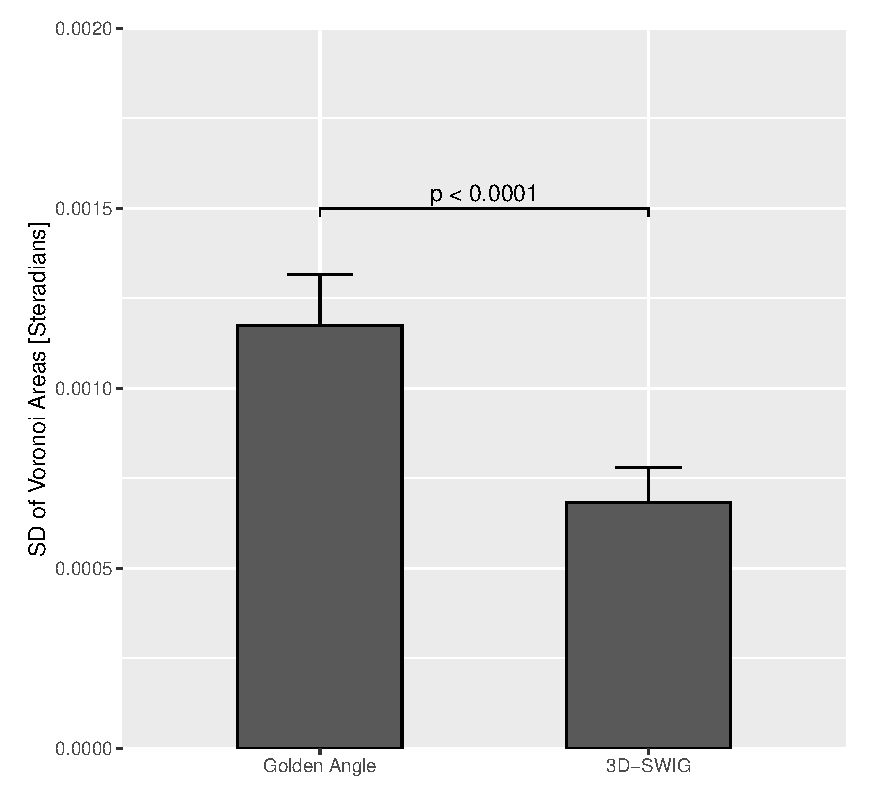
\includegraphics[width=0.75\textwidth]{Rplot02}
    \caption{The standard deviation of Voronoi cell areas was used to assess k-space uniformity after binning. The data from the three subjects were reconstructed into 20 cardiac bins and 3 respiratory bins, resulting in a total of 180 bins, and all Voronoi cell areas were calculated for each bin. A lower value indicates a more uniform k-space.}
    \label{fig:study4_2}
\end{figure}


\chap{Discussion}

 The purpose of this chapter is to provide some additional considerations and the author's own reflections on the methods and their limitations, which has not already been covered in the previous sections.

\sect{Physiological binning when using the golden angle}
The golden angle provides an approximately uniform distribution of k-space readouts for an arbitrary number of readouts. This means that an arbitrary number of readouts will provide a good k-space coverage, as opposed to linear radial methods, which would require an \emph{a priori} decision regarding the number of readouts. The idea is that every new line will provide additional k-space coverage where it is most needed, i.e. each succeeding readout will fill one of the largest gaps in k-space. This has sometimes been interpreted to mean that an arbitrary non-continuous subset of readouts will constitute a uniform k-space coverage. If the number of readouts is large, it could be expected that a \textbf{random} subset is near uniform if readouts are chosen with equal probability. However, in real applications, we are rarely interested in random subsets. Rather, we use some physiological motion signal, such as an ECG or respiratory signal to select readouts. Such functions are often periodic to some degree, meaning that we periodically discard and reject readouts. This tends to create gaps in the sampling pattern, resulting in severe image artifacts, see Figure~\ref{fig:swig_binning}.
\begin{figure}[htbp]
    \centering
    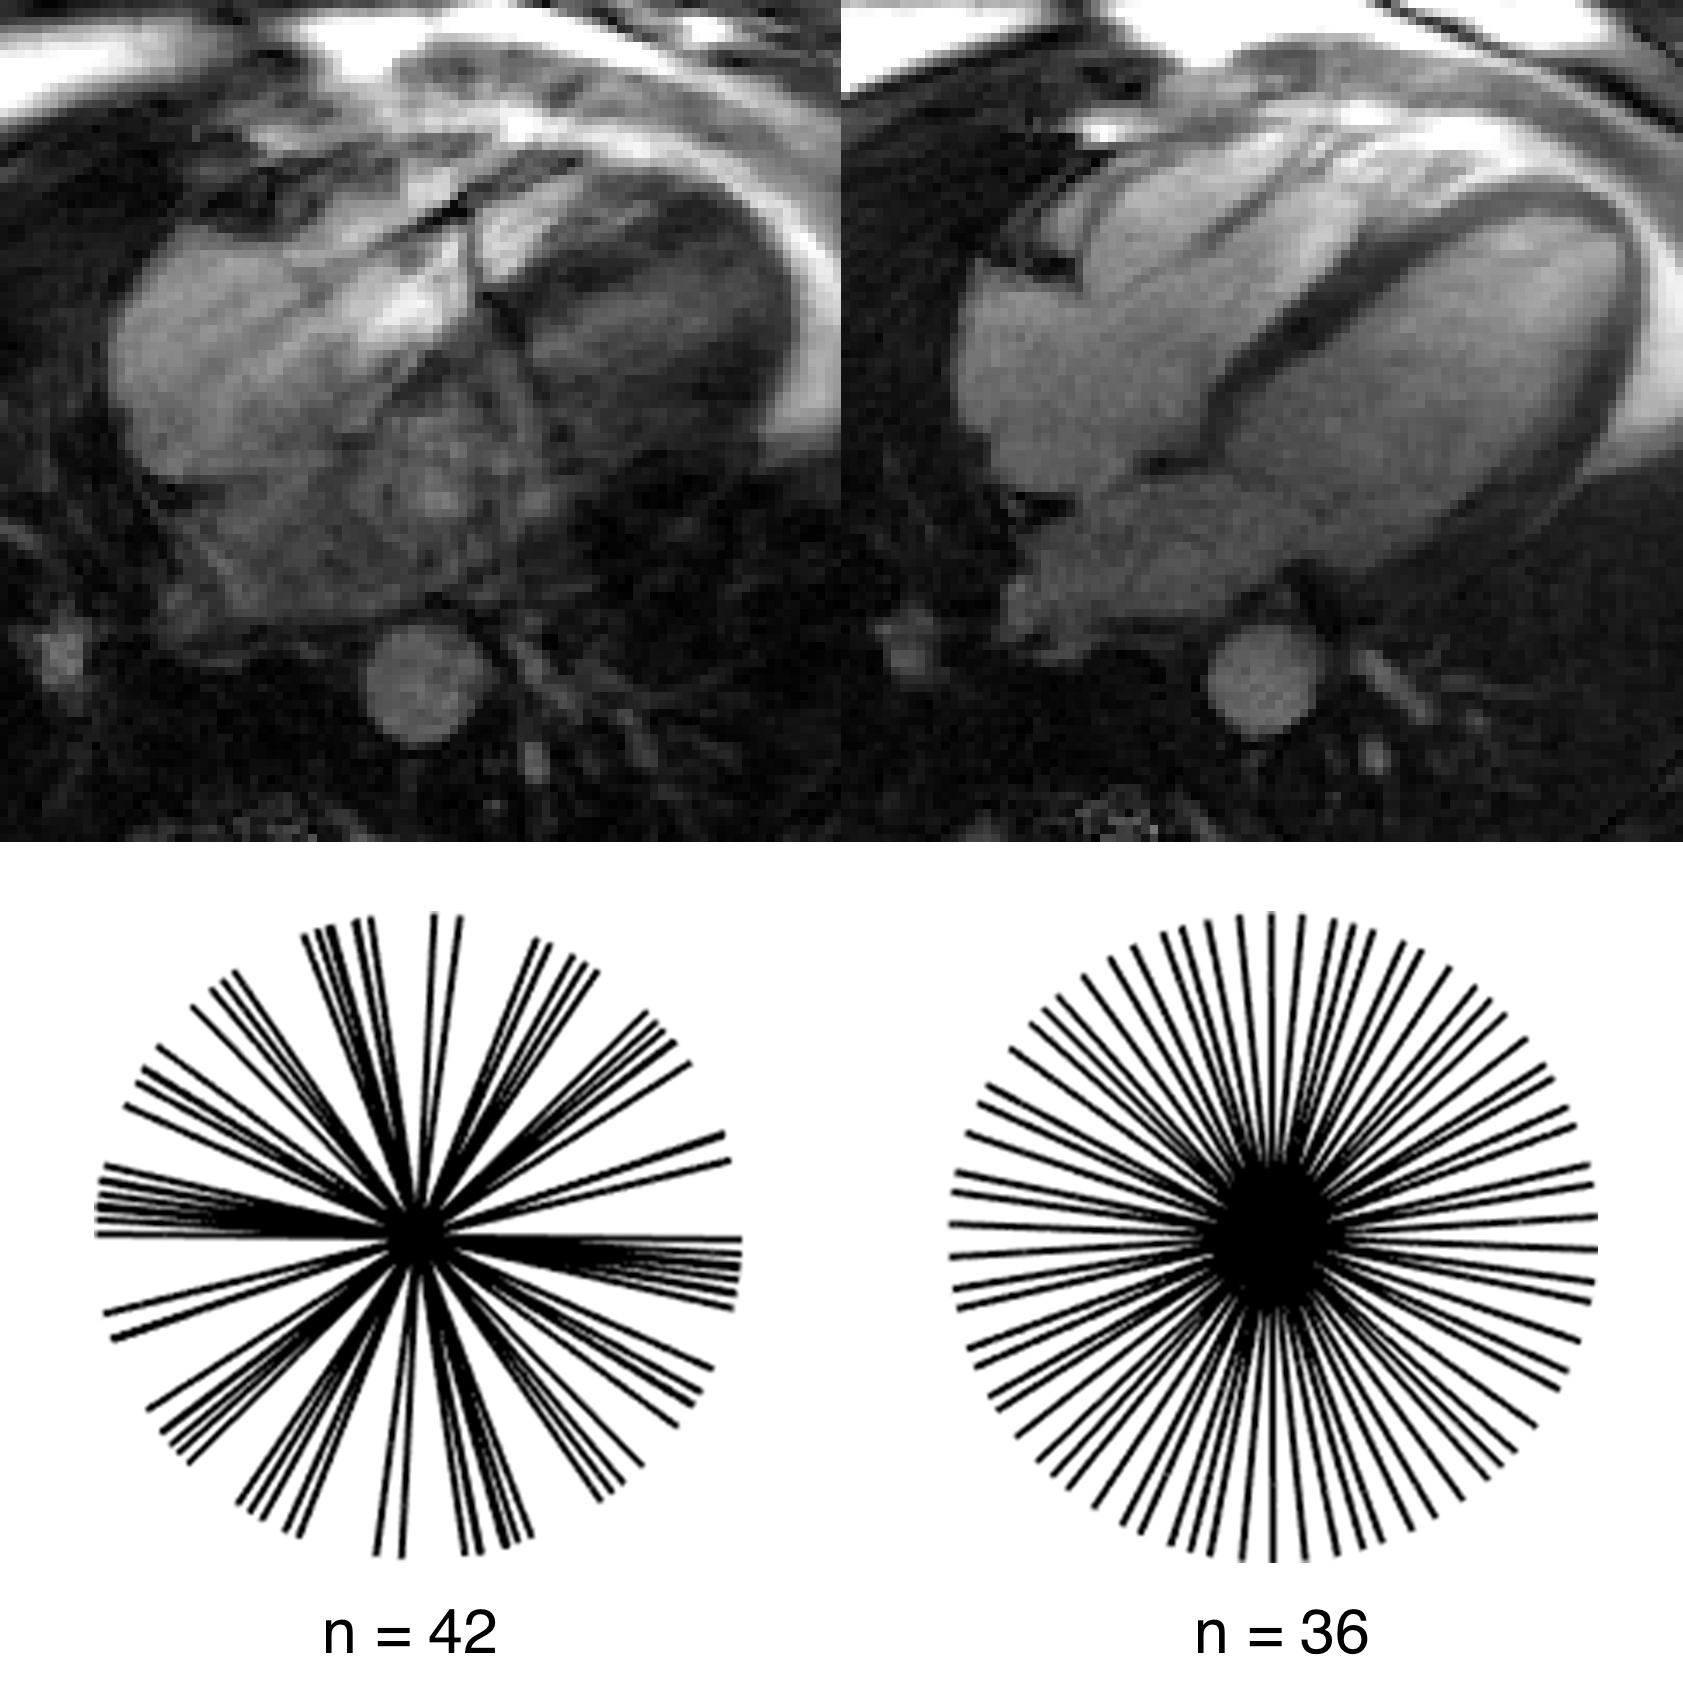
\includegraphics[width=0.75\textwidth]{with_traj.png}
    \caption{Examples of ECG-binning of the conventional golden-angle profile ordering (left) and the 2D-SWIG profile ordering (right).}
    \label{fig:swig_binning}
\end{figure}
Using the SWIG method, we can adapt the sampling to a physiological signal, such as the ECG, as described in this thesis, but in theory, it should be possible to adapt the acquisition to any motion signal that we can acquire at imaging time. Recent research has lead to the development of the Doppler ultrasound (DUS) \Nomenclature{DUS}{Doppler ultrasound} gating device for fetal cardiac gating~\cite{Kording2018}. Such a device could potentially also be used to prospectively measure respiratory motion, enabling multidimensional SWIG-imaging.

\sect{Underestimation of transmitral blood flow using SWIG-PC}
One of the findings in \textbf{Study III} was that SWIG agrees with Doppler echocardiography for myocardial tissue velocity measurements, but that the transmitral blood flow velocity were underestimated. This finding is surprising, as the myocardial tissue velocities were expected to be a more challenging target with regards to accuracy. The myocardial velocity peak in the early filling (e') is very narrow, so a low temporal footprint is expected to be needed in order to capture the peak velocity accurately. The velocity peaks in the transmitral blood flow are much broader, so such a high temporal resolution should not be needed. Yet the results clearly show a systematic underestimation of the transmitral blood flow. While more work is warranted, a possible explanation for this is that the slice planning was sub-optimal. Recent work has proposed slice tracking for phase~contrast imaging of the valves~\cite{Seemann2019}, which is a method that could potentially be adopted into the SWIG-PC method. Another possible solution would be to, instead of planning in a short-axis orientation, use a long-axis image with in-plane velocity encoding, where the active measurement volume could be placed in an optimal position to capture the transmitral inflow. 

\sect{Limitations}
This thesis would not be complete without a reflection on its limitations. 

In \textbf{Study I}, the sample size was limited and comprised mainly health volunteers. A more systematic evaluation would be necessary to determine the clinical utility of the method. Preferably with paired evaluations between CTA and MRI, to be able to estimate the sensitivity and specificity of each method. Another important methodological limitation is the blinding of the observers who were asked to score the images. When comparing a Cartesian and radial method, it is hard to blind the observer to the method, as radial images often has a very characteristic look. A possible solution could have been to calculate a mask outside of the body to hide the streaks in the air, which may be the biggest giveaway and, at the same time, contributing little to the utility of the images.
In \textbf{Study II}, a major limitation was the lack of systematic evaluation of the method \emph{in vivo}, as only a single subject was imaged. Another important limitation that should be mention is that k-space uniformity could have been a confounding factor. The hypothesis was that the improved image quality was due to reduced angular differences within a 2-TR phase cycle. However, as the sampling trajectory was changed, this could also have affected the sampling uniformity and thereby the image quality. It may have been useful to use an external measure, such as a field camera, in an attempt to quantify how much of the improvement came from the reduced angular switching.
In \textbf{Study III}, tissue velocity measurements were compared between CMR and Doppler echocardiography. Initial results from the pilot study suggested that the CMR overestimated tissue velocities compared to Doppler echocardiography. However, no comparisons were made to a gold standard. A suitable gold standard for simultaneous evaluation of both measurements could have been ultrasonic micrometry \cite{Kokubo1995}.
In \textbf{Study IV}, a major limitation was the lack of systematic evaluation \emph{in vivo}. As the images were reconstructed using a compressed sensing algorithm with temporal regularization, it is important to verify that temporal smoothing did not affect the measurement of ventricular volumes. This could have been verified against measurements of the ventricular volumes using breath-held two-dimensional cine.

A limitation for all studies involving healthy volunteers was that volunteer recruitment was made mostly through the author's own network of contacts, and many volunteers were either researchers or medical professionals. This may have contributed to some systematic bias, as most volunteers were young and of above-average fitness, as opposed to the typical patient referred for cardiac MRI.

\sect{Ethical considerations}
Most of the thesis involved some degree of development of novel clinical methods. As such, they have to ultimately be evaluated in human subjects, both healthy volunteers and patients. All studies which involved human subject were performed in accordance with the Declaration of Helsinki~\cite{WMA2013}.

\subsect{Healthy volunteers}
Ethical permits were in place for evaluating the methods, both for healthy volunteers and patients. It is important to note that there existed dedicated ethical approval to test all methods in both healthy volunteers and patients, as there may exist situations where it may be ethical to evaluate a method in a patient but not a healthy volunteer.
All volunteers gave informed, written consent to participate. Their personal information was treated confidentially as required by both ethical guidelines and the law. Most of the research in these studies were performed on raw k-space data. Consequently, the data could be anonymized, i.e., irreversibly separated from any identifying information.

\subsect{Patients}
In the studies which involved patients, all necessary steps were taken to ensure their privacy and integrity. The patients involved in \textbf{Study I} were prospectively included based on their clinical referral. In \textbf{Study II}, no patients were involved. In \textbf{Study III} and \textbf{Study IV}, patients were retrospectively included from the body of patients that had agreed to have their data used for clinical research. In the case of the prospectively included patients, their decision to participate meant that they were subject to an additional MRI scan. Importantly, this did not delay the care they would have received had they not chosen to participate. In the case of retrospectively included patient, their participation did not alter the clinical care they received in the healthcare system.

\sect{Safety}
MRI is a non-invasive method of imaging that does not expose the subject to ionizing radiation. As such, MRI should be considered a safe imaging modality. No long-term biological effects have been associated with MRI. The short-term effects experienced by some patients may include claustrophobia, magnetophosphenes (an optical illusion where the subject experiences light flashes), peripheral nervous stimulation, and heating. None of the research protocols included contrast agents or other drugs. In cases where patients received a contrast agent, this was part of the clinical routine and administered by a trained professional. None of the scanner's safety features were disengaged during the scanning of patients and healthy volunteers, and the most recent safety guidelines were followed at all times~\cite{Kanal2013,Greenberg2020}.

\sect{Future perspectives}
Although golden-angle based methods have been around since 2007, they have yet to find mainstream adoption. There is still a strong bias towards conventional Cartesian methods. Many sequence development environments, and image reconstruction tools have not yet adapted to advanced sampling techniques, and the vendors have not always caught up with the latest research. However, the research community have taken it upon themselves to develop sequence programming environments~\cite{Layton2017,Skare2017:ISMRM}, and open-source image reconstruction toolboxes such as BART~\cite{Uecker2015:ISMRM} and Gadgetron~\cite{Hansen2013}, which can be integrated into the scanner workflow and even enable online image reconstruction in the cloud~\cite{Xue2015}.

An elusive target has for long been the ``five minute MRI'', i.e., to perform a comprehensive cardiac MRI examination in five minutes, as opposed to 45 minutes or even an hour, which is the norm today. Professor Daniel K. Sodickson, at NYU Langone Health, has spoken about a future where the patient goes in the scanner, and data is continuously acquired. When the patient has left, powerful computational computers are put to work, or leveraging the power of the cloud, to process the data and create the imaging slices and contrasts needed for the clinical diagnosis. Further along, machine learning might directly analyze the images in some other feature space, and not necessarily as images. Major advances in machine learning are already underway with the advent of the AutoMAP-method~\cite{Zhu2018}, which learns domain transfer from the k-space to the image domain using neural networks and can in the process learn to compensate for image artifacts. Both the AutoSEQ~\cite{Zhu2018:ISMRM} and MRZero~\cite{Loktyushin2020} methods have taken things a step further. Both are using Bayesian reinforcement learning to learn pulse sequences generation without user interaction. Golden-angle based methods may very well play a part in these developments, as they are particularly suited for volumetric imaging, and their golden nature lends itself to continuous sampling where each new readout will provide unique information. With the aforementioned developments in terms of sequence development environments, reconstruction algorithms, and more readily available compute power, it is likely that non-Cartesian methods will have an essential place in the future for cardiovascular MRI.
\chap{Conclusions}
In addition to utilizing golden-angle in novel applications, the thesis also explored methods for remedying problems that are usually associated with golden-angle radial sampling, such as eddy-current induced image artifacts and sampling non-uniformity when combined with physiological binning. The studies conducted as part of this thesis suggest that these problems can be overcome, making golden-angle imaging an attractive solution for cardiovascular MRI, especially for highly efficient high-temporal resolution imaging. This may push the boundary for the capabilities of cardiovascular MRI, or robust free-breathing applications, which can be of great benefit for under-served patient groups.

The specific conclusions for Studies I-IV were:
\begin{enumerate}[I.]
    \item The golden-angle radial trajectory can provide robustness to motion and flow when compared to a conventional Cartesian imaging method. The proposed method allowed for imaging the pulmonary vasculature with thin slices free from artifacts.
    \item Generalization of the generating function for the three-dimensional golden-angle profile ordering can be used to create golden-angle-like profile orderings with reduced angular steps between readouts, which leads to less eddy-current induced image artifacts and less sensitivity to off-resonance.
    \item The modified two-dimensional golden-angle method, SWIG, can be used in combination with a phase-contrast readout to enable high temporal resolution imaging of the diastolic function of the heart, with good agreement when compared to Doppler echocardiography.
    \item The modified, three-dimensional golden-angle method, 3D-SWIG, can improve sampling uniformity at high undersampling factors, which was demonstrated by performing three-dimensional free-breathing whole heart cine imaging in less than a minute.
\end{enumerate}



\clearpage

% ==================================
% ACKNOWLEDGMENTS
% ==================================
\backmatter
\chap{Acknowledgements}
I would like to acknowledge my principal supervisor \textbf{Andreas Sigfridsson}. I have thoroughly enjoyed learning from you. Over the years, \textbf{Andreas} and I have developed a tendency to brainstorm during regular conversations. We rarely take notes, but the good ideas get separated from the bad through a process of natural selection. I profusely apologize to anyone who has been caught in the crossfire.

I would also like to acknowledge my co-supervisor \textbf{Martin Ugander} as well as Professors \textbf{Kenneth Caidahl} and \textbf{Henrik Engblom} for their exemplary mentorship. \textbf{Martin} might not have been as involved in the nitty-gritty, but his presence is felt all through this thesis. \textbf{Kenneth} has been watching over the process and generously shared his experience. \textbf{Henrik} has been a late addition to the team, but our discussions so far have been tremendously helpful. 

A special dedication goes out to the current and former members of the Karolinska CMR Group. In addition to those above, I would like to mention, in no particular order; \textbf{Karen Holst}, \textbf{Jannike Nickander}, \textbf{Björn Wieslander}, \textbf{Magnus Lundin}, \textbf{Simon Thalén}, \textbf{João Ramos}, \textbf{Maren Maanja}, \textbf{Raquel Themudo}, \textbf{Peder Sörensson}, \textbf{Eva Maret}, \textbf{Jenny Rasck}, \textbf{Sofie Olsson}, \textbf{Márcia Ferreira}, \textbf{Elina Malkeshi}, \textbf{Rebecca Almqvist}, \textbf{Mariana Soares}, \textbf{Mahmood Farasati}, \textbf{Goran Abdula}, \textbf{Fredrika Fröjdh}, \textbf{Daniel Loewenstein} and \textbf{Johan von Scheele}.

I extend a special thanks to; \textbf{Jannike}, who has the highest SNR of any person I have ever met. We all know it, but I'm willing to put it in writing; You will go far! \textbf{Karen}, who showed me the ropes and mentored me in my early days as a master student and helped me hit the ground running. \textbf{Jenny}, who was the one who first taught me how to operate an MRI scanner. \textbf{João}, for being my main collaborator on so many projects and for being part of the final sprint of the thesis writing together with \textbf{Maren} and \textbf{Magnus}. You all have offered a great deal of moral support.
\clearpage
Moreover, I would like to thank everyone that contributed as co-authors to the papers included in this thesis and has not already been mentioned; \textbf{Roberto Vargas Paris}, \textbf{Maria Eriksson}, \textbf{Peter Lindholm} and \textbf{Sven Nyrén}. \textbf{Maria} has shown great trust in me, which has helped my professional career. \textbf{Peter} has been a mentor for me in many ways. For that, I owe them both my gratitude.


There are lots of people who haven't been directly involved in the writing of this thesis, but that have made a lasting impression in one way or another. To them, I would like to extend my sincerest thank you.

To my co-authors on the papers that didn't make in into this thesis, in particular \textbf{Koshiar Medson}, \textbf{Deepa Gopalan}, \textbf{Ursula Reiter}, \textbf{Gert Reiter}, \textbf{Ning Jin}, \textbf{Mikael Melin}, \textbf{Patrik Sundblad}, \textbf{Viktoria Skott} and \textbf{Susanne Rysz}.

To my scientific role model, \textbf{Peter Kellman}.

To the people in the industry that I have had the pleasure to work with. In particular \textbf{Frederik Testud}, \textbf{Kelvin Chow} and \textbf{Davide Piccini}. A honorable mention to the service engineers who mostly believed me when I told them something was wrong with the scanner, but never once blamed me for causing it; \textbf{Denny Hägg}, \textbf{Marko Sinadinovic}, \textbf{Michel Ten Heggeler} and \textbf{Akal Yehualashet}.

To the people I have met through conferences and travels, in particular \textbf{Johannes Töger}, \textbf{Kerstin Hammernik} and \textbf{John Heerfordt}.

To all my teachers. To all my students, and in particular the ones I have had the pleasure to supervise; \textbf{Reenalyn Borromeo}, \textbf{Emil Olsson}, \textbf{Rebecka Herterich}, \textbf{Anna Sumarokova}, \textbf{Adham Belbaisi}, \textbf{Max Kim} and \textbf{Amanda Ullvin}.

To \textbf{Elina Renhorn} for standing beside me with your never-ending support.

To my mother \textbf{Kerstin}, my father \textbf{Thomas} and my brother \textbf{Michael}.

To my nieces \textbf{Heylie} and \textbf{Milla} to whom this thesis is dedicated.
\newpage

% ==================================
% CHAPTER: REFERENCES
% ==================================
\bibliographystyle{vancouver}
\bibliography{references}  % Link to bibtex file
\end{document}
% ==================================
% PART II: RESEARCH PAPERS
% ==================================
\newpage
\pagenumbering{gobble}

% ==================================
% INSERT PAPERS
% ==================================
% Comment-out the 'includepdf' to compile faster while you are writing.
%
% ------------------
% PAPER I
% ------------------
\thispagestyle{empty}
\vspace*{2cm}  % IMPORTANT: Increase by 2cm each time.
\hfill{}
\marginpar{\rulebox{I}} % Change the Roman number here
\vfill
\cleardoublepage
%\includepdf[pages=-,width=\textwidth,pagecommand={\thispagestyle{plain}},clip,viewport=53 56 560 774]{papers/Fyrdahl_et_al-2018-Magnetic_Resonance_in_Medicine.pdf}

% ------------------
% PAPER II
% ------------------
\thispagestyle{empty}
\vspace*{4cm}  % IMORTANT: Increase by 2cm each time.
\hfill{}
\marginpar{\rulebox{II}} % Change the Roman number here
\vfill
\cleardoublepage
%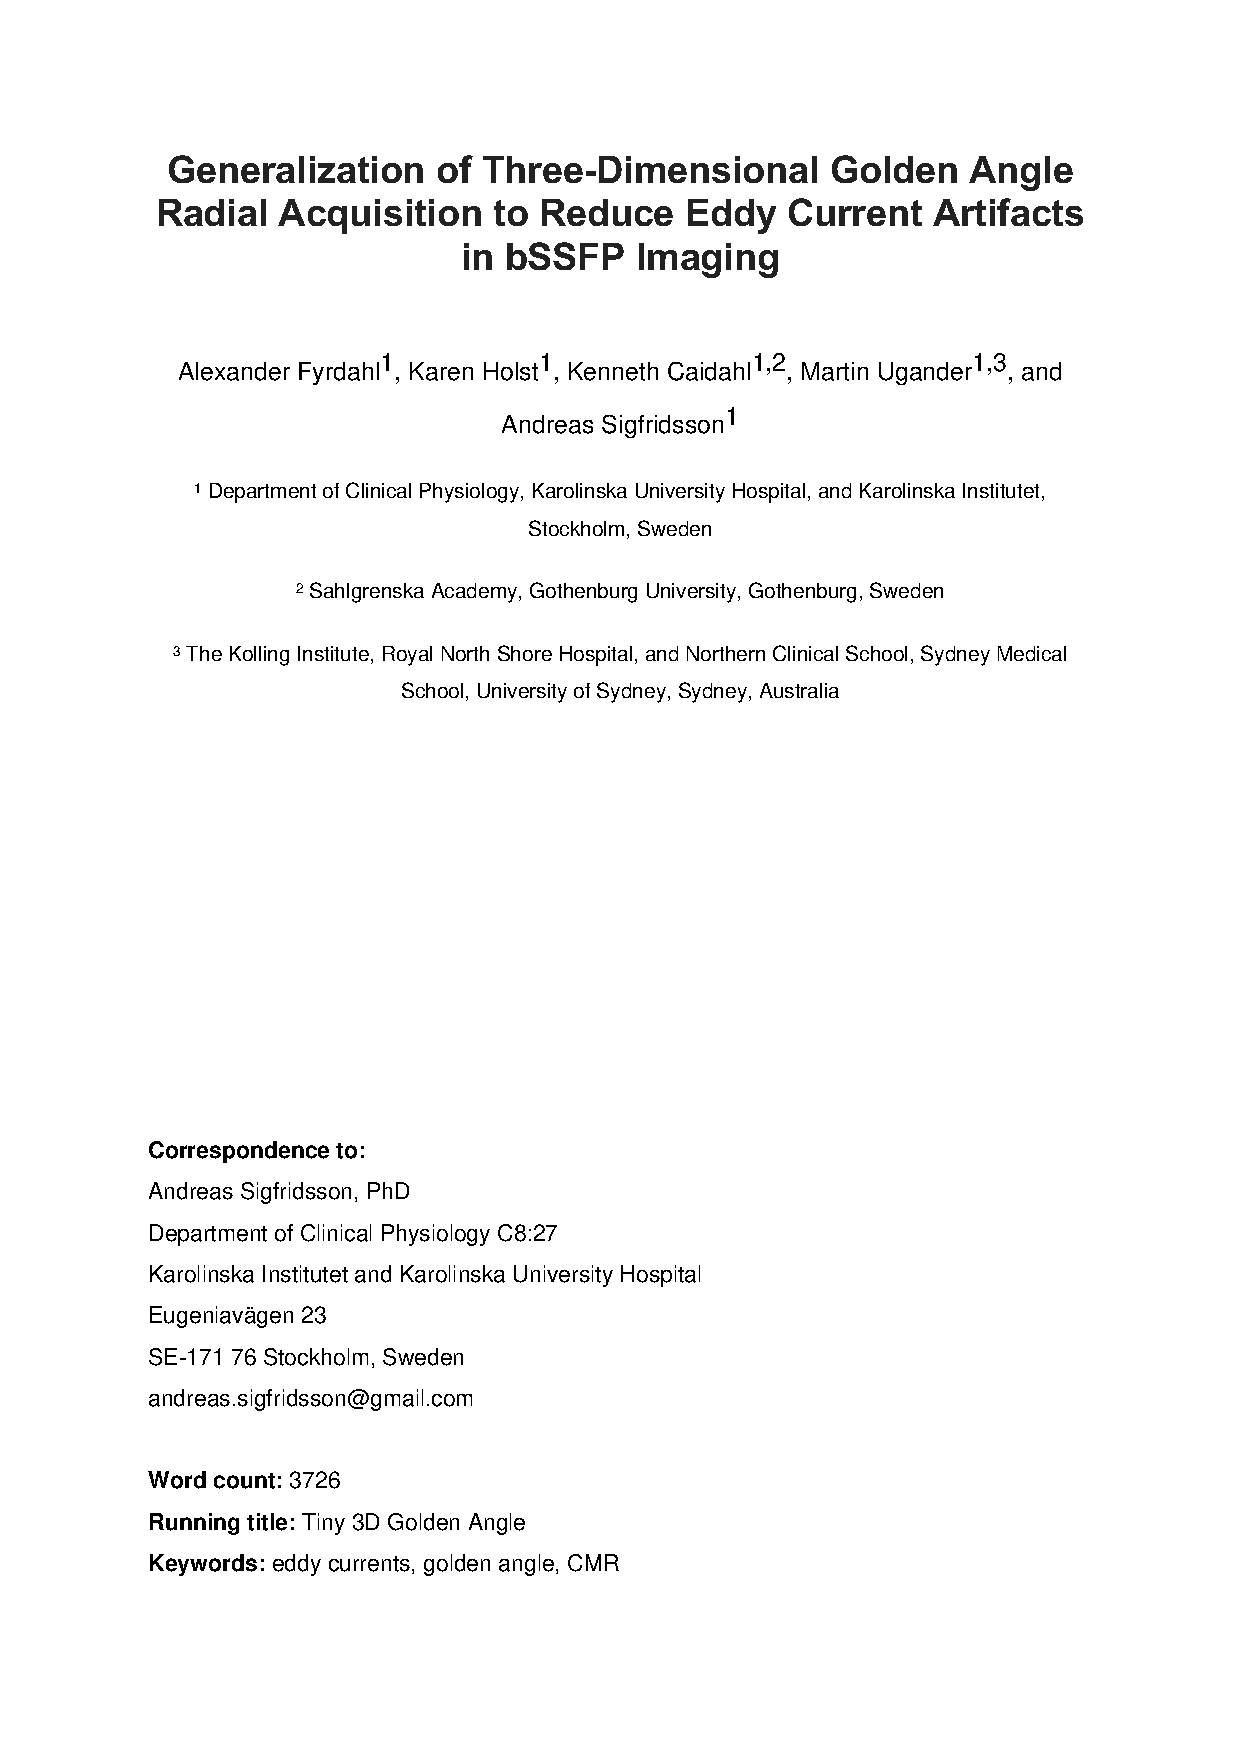
\includepdf[pages=-,width=1.25\textwidth,pagecommand={\thispagestyle{plain}}]{papers/Study_II_Manuscript.pdf}

% ------------------
% PAPER III
% ------------------
\thispagestyle{empty}
\vspace*{6cm}  % IMPORTANT: Increase by 2cm each time.
\hfill{}
\marginpar{\rulebox{III}} % Change the Roman number here
\vfill
\cleardoublepage
%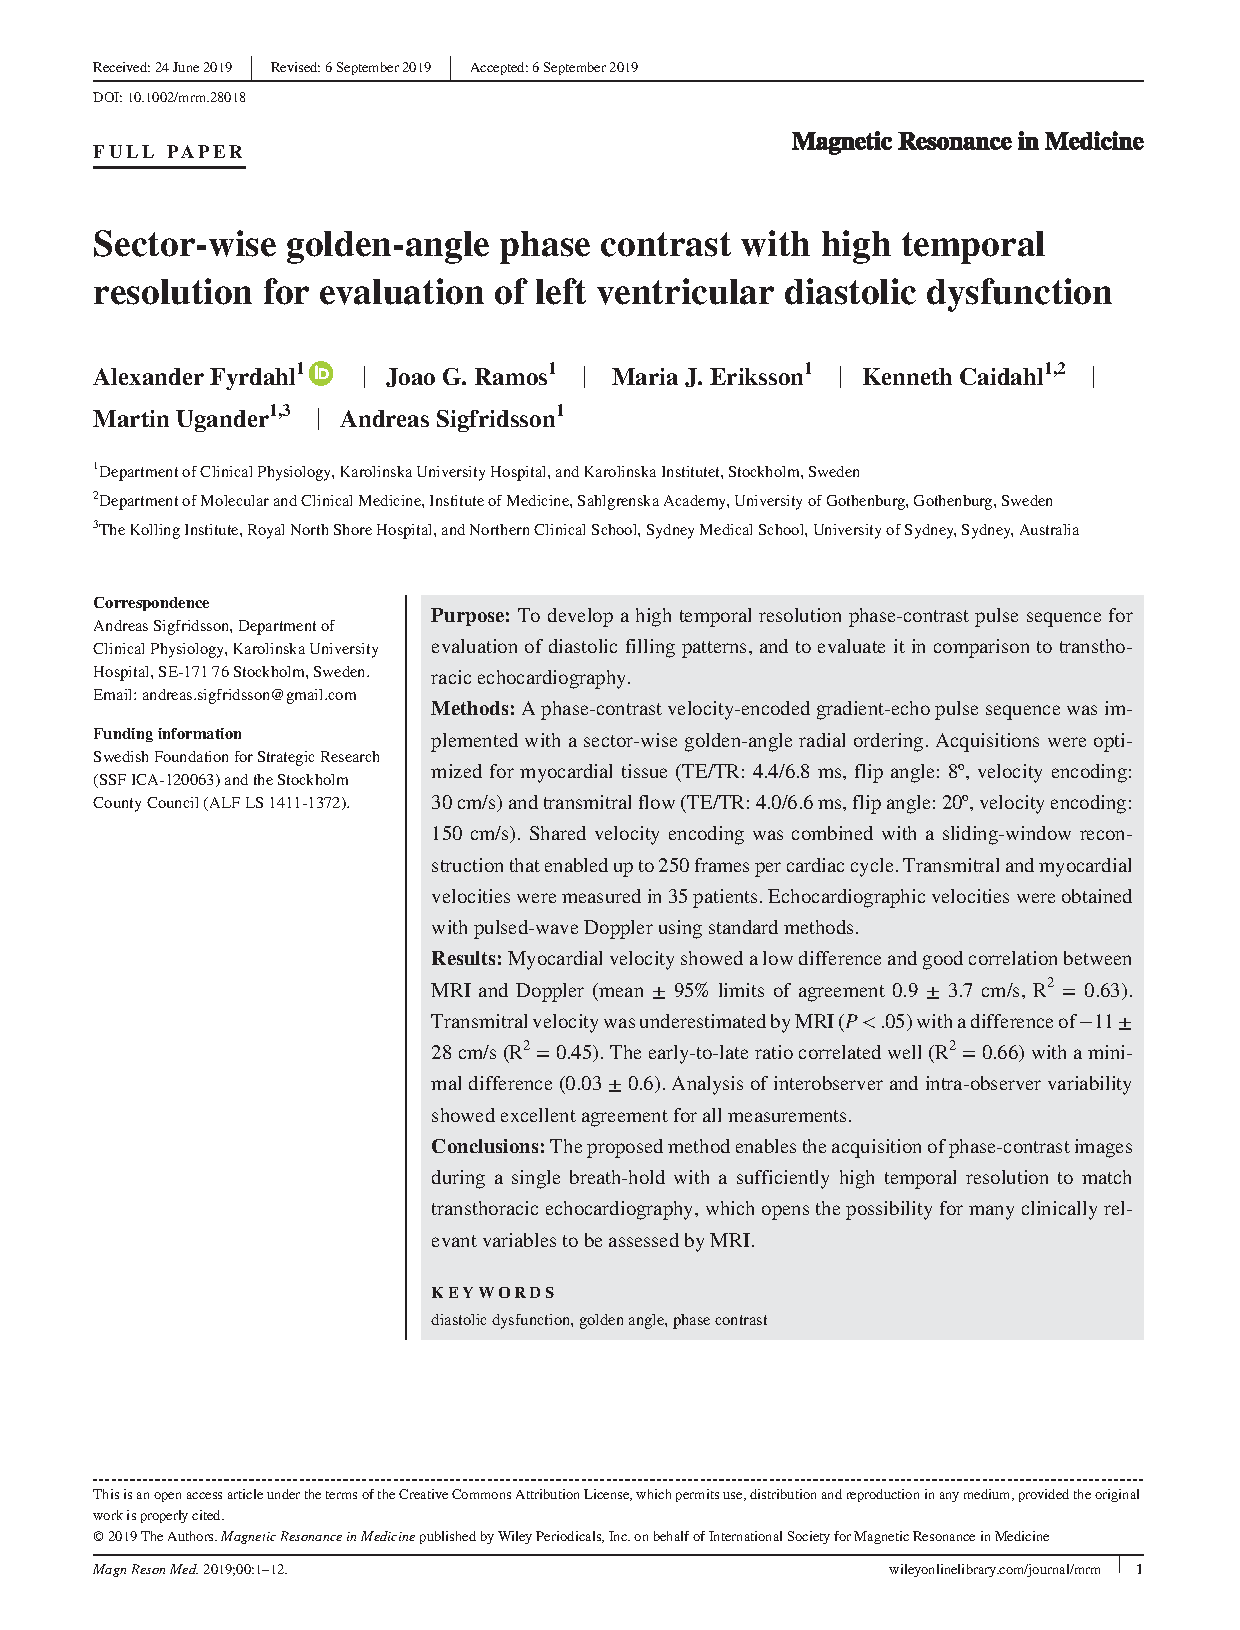
\includepdf[pages=-,width=1.0\textwidth,pagecommand={\thispagestyle{plain}},clip,viewport=44 43 552 762]{papers/Fyrdahl_et_al-2019-Magnetic_Resonance_in_Medicine.pdf}

% ------------------
% PAPER IV
% ------------------
\thispagestyle{empty}
\vspace*{8cm}  % IMPORTANT: Increase by 2cm each time.
\hfill{}
\marginpar{\rulebox{IV}} % Change the Roman number here
\vfill
\cleardoublepage
%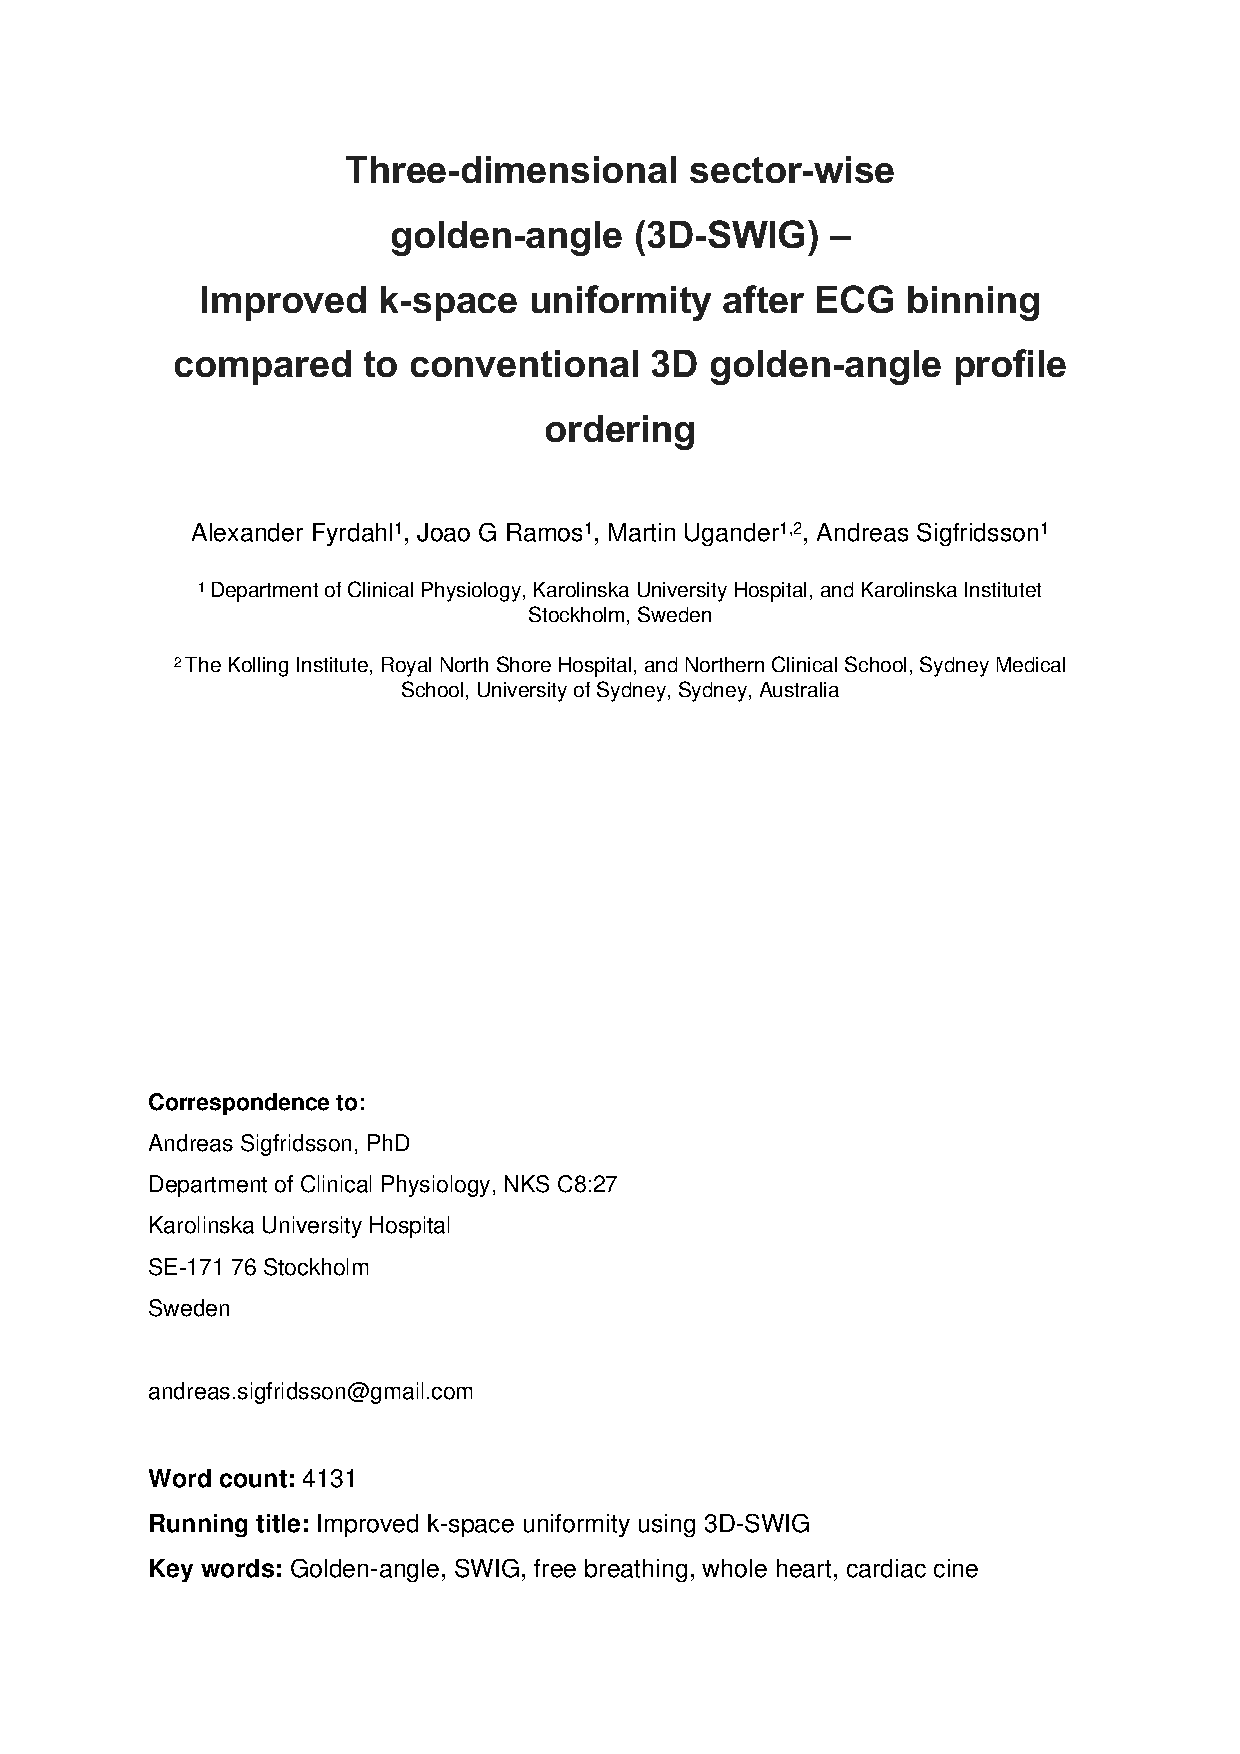
\includepdf[pages=-,width=1.25\textwidth,pagecommand={\thispagestyle{plain}}]{papers/Study_IV_Manuscript.pdf}
\end{document}